%%%%%% Compile with: xelatex wil-report.tex (run twice for ToC, then bibtex, then xelatex twice more)
\documentclass[12pt,oneside,openright,a4paper]{cpe-english-project}

\usepackage{polyglossia}
\setdefaultlanguage{english}
\setotherlanguage{thai}
\defaultfontfeatures{Path=./fonts/,Mapping=tex-text,Scale=1.0,LetterSpace=0.0}
\newfontfamily\thaifont[
  Path=./fonts/,
  Script=Thai,
  Scale=1.23,
  Extension=.ttf,
  UprightFont=*-Regular,
  BoldFont=*-Bold,
  ItalicFont=*-Italic,
  BoldItalicFont=*-BoldItalic
]{THSarabunNew}
\setmainfont[
  Path=./fonts/,
  Extension=.ttf,
  UprightFont=*-Regular,
  BoldFont=*-Bold,
  ItalicFont=*-Italic,
  BoldItalicFont=*-Bold-Italic,
  Scale=1.0,
  LetterSpace=0,
  WordSpace=1.0,
  FakeStretch=1.0
]{Times New Roman}
\emergencystretch=10pt

\usepackage{float}
\usepackage{longtable}
\usepackage{booktabs}
\usepackage{array}
\usepackage{enumitem}
\setlist[itemize]{noitemsep, topsep=2pt}
\setlist[enumerate]{noitemsep, topsep=2pt}

%%%%%%%%%% Personal metadata %%%%%%%%%%
\def\disstitleone{Automated Data Ingestion and Pipeline System}
\def\disstitletwo{for AI Model Training}
\def\dissauthor{MS. Kwinyarut Poungsangthanakul}
\def\dissauthortwo{Mr. Parit Leelasetawong}
\def\dissauthorthree{}

\def\dissdegree{Bachelor of Engineering}
\def\dissdegreeabrev{B.Eng}
\def\dissyear{2026}
\def\thaidissyear{2569}

\def\dissadvisor{Dr. Aye Hninn Khine}
\def\disscoadvisor{}
\def\disscoadvisortwo{}
\def\disscoadvisorthree{}
\def\disscommitteetwo{Dr. Piyanit Ua-areemitr}
\def\disscommitteethree{Mr. Naveed Sultan}
\def\disscommitteefour{}

\def\worktype{Project}
\def\disscredit{18}

\def\fieldofstudy{Computer Engineering}
\def\department{Computer Engineering}
\def\faculty{Engineering}

\def\thaifieldofstudy{วิศวกรรมคอมพิวเตอร์}
\def\thaidepartment{วิศวกรรมคอมพิวเตอร์}
\def\thaifaculty{วิศวกรรมศาสตร์}

\def\appendixnames{Appendix}

\def\thaiworktype{ปริญญานิพนธ์}
\def\thaidisstitleone{ระบบการนำเข้าข้อมูลและสายงานประมวลผลแบบอัตโนมัติ}
\def\thaidisstitletwo{สำหรับการฝึกแบบจำลองปัญญาประดิษฐ์}
\def\thaidissauthor{นางสาว กวินญรัตน์ พ่วงแสงธนกุล}
\def\thaidissauthortwo{นาย ปริตต์ ลีลาเศรษฐวงศ์}
\def\thaidissauthorthree{}
\def\thaidissadvisor{ดร. เอ หนิน ขิ่น}
\def\thaidisscoadvisor{}
\def\thaidisscoadvisortwo{}
\def\thaidisscoadvisorthree{}
\def\thaidissdegree{วิศวกรรมศาสตรบัณฑิต}

\linespread{1.15}

\renewcommand{\topfraction}{0.85}
\renewcommand{\textfraction}{0.1}

\newtheorem{theorem}{Theorem}
\newtheorem{lemma}{Lemma}
\newtheorem{corollary}{Corollary}

\def\QED{\mbox{\rule[0pt]{1.5ex}{1.5ex}}}
\def\proof{\noindent\hspace{2em}{\itshape Proof: }}
\def\endproof{\hspace*{\fill}~\QED\par\endtrivlist\unskip}


\begin{document}
\pdfstringdefDisableCommands{%
\let\MakeUppercase\relax
}
\begin{center}
  
\includegraphics[width=2.8cm]{logo02.jpg}
\end{center}
\vspace*{-1cm}

\maketitlepage
\makesignaturepage

%%%%%%%%%%%%%%%%%%%%%%%%%%%%%%%%%%%%%%%%%%%%%%%%%%%%%%%%%%%%%%
%%%%%%%%%%%%%%%%%%%%%% English abstract %%%%%%%%%%%%%%%%%%%%%%
%%%%%%%%%%%%%%%%%%%%%%%%%%%%%%%%%%%%%%%%%%%%%%%%%%%%%%%%%%%%%%
\abstract

The growing demand for AI at Siam.AI Cloud requires large, high-quality datasets that can be processed reliably across many different formats. However, current data preparation workflows are fragmented, largely manual and error-prone especially for Thai-language data. This project addresses these challenges by building an end-to-end, open-source, on-premise pipeline that takes raw data in various formats and converts it into clean, standardized outputs ready for training large language models.

The system uses a Data Lakehouse design with MinIO for scalable object storage, PostgreSQL for metadata and processing logs and Apache Airflow for automating the entire workflow. The pipeline handles ingestion, cleaning, normalization, deduplication and quality validation across various data types, with a primary focus on the NECTEC corpus, covering formats such as JSONL, Parquet, CSV, TXT, PDF documents and audio recordings. For PDFs, the pipeline employs an OCR model deployed in order to extract text from scanned and digitally-encoded Thai documents through a dual-pass strategy, while attempting fast text extraction first and falling back to OCR when encoding issues are detected. Moreover, the audio pipeline leverages an ASR-Whisper model to transcribe Thai speech, incorporating a multi-level quality checking system capable of validating output even in the absence of ground truth labels. Pipeline health, storage usage and data quality are monitored in real time through Prometheus and Grafana dashboards.

The resulting system reduces manual effort, ensures consistent data quality across all processing stages, and produces standardized JSONL outputs ready for AI model training. It establishes a reusable foundation for Thai LLM development and future data engineering work at Siam AI Cloud.

\begin{flushleft}
\begin{tabular*}{\textwidth}{@{}lp{0.8\textwidth}}
\textbf{Keywords}: & Data Ingestion / Data Lakehouse / Apache Airflow / OCR / ASR / Thai NLP
\end{tabular*}
\end{flushleft}
\endabstract

%%%%%%%%%%%%%%%%%%%%%%%%%%%%%%%%%%%%%%%%%%%%%%%%%%%%%%%%%%%%%%
%%%%%%%%%% Thai abstract %%%%%%%%%%%%%%%%%%%%%%%%%%%%%%%%%%%%%
%%%%%%%%%%%%%%%%%%%%%%%%%%%%%%%%%%%%%%%%%%%%%%%%%%%%%%%%%%%%%%
{
\XeTeXlinebreaklocale "th_TH"
\XeTeXlinebreakskip = 0pt plus 1pt
\thaifont
\thaiabstract

การเติบโตอย่างรวดเร็วของเทคโนโลยีปัญญาประดิษฐ์ใน Siam.AI Cloud ส่งผลให้เกิดความต้องการชุดข้อมูลขนาดใหญ่และมีคุณภาพสูง ซึ่งสามารถประมวลผลข้ามรูปแบบที่หลากหลายได้อย่างมีเสถียรภาพ อย่างไรก็ตาม กระบวนการเตรียมข้อมูลในปัจจุบันยังมีลักษณะกระจัดกระจาย ต้องอาศัยการดำเนินการแบบแมนนวลและมีความเสี่ยงต่อความผิดพลาดสูงโดยเฉพาะอย่างยิ่งกับข้อมูลภาษาไทย โครงงานนี้มีวัตถุประสงค์เพื่อแก้ไขปัญหาดังกล่าวผ่านการพัฒนาระบบสายงานประมวลผลแบบครบวงจร (End-to-end Pipeline) ประเภทโอเพนซอร์ส (Open-source) ที่ติดตั้งใช้งานภายในพื้นที่ปฏิบัติการ เพื่อรวบรวม แปลง และเตรียมข้อมูลดิบจากหลากหลายรูปแบบให้เป็นผลลัพธ์มาตรฐานที่สะอาดและพร้อมใช้งานสำหรับการฝึกแบบจำลองภาษาขนาดใหญ่ (Large Language Models: LLMs)\par

ระบบถูกออกแบบภายใต้แนวคิดคลังข้อมูลแบบผสมผสานระหว่างแหล่งเก็บข้อมูลขนาดใหญ่และคลังข้อมูลเชิงวิเคราะห์ (Data Lakehouse) โดยใช้ MinIO เป็นระบบจัดเก็บข้อมูลแบบวัตถุที่รองรับการขยายตัว ใช้ฐานข้อมูลเชิงสัมพันธ์ PostgreSQL สำหรับจัดการเมทาดาทาและบันทึกการประมวลผล และใช้ Apache Airflow ในการควบคุมการทำงานแบบอัตโนมัติทั้งระบบ รองรับขั้นตอนการนำเข้าข้อมูล การทำความสะอาดข้อมูล การปรับมาตรฐาน การขจัดข้อมูลซ้ำ และการตรวจสอบคุณภาพ ครอบคลุมข้อมูลหลายประเภท โดยมุ่งเน้นที่คลังข้อมูล NECTEC ซึ่งประกอบด้วยรูปแบบไฟล์ JSONL, Parquet, CSV, TXT, เอกสาร PDF และไฟล์เสียง\par

สำหรับการประมวลผลเอกสาร PDF ระบบได้ประยุกต์ใช้แบบจำลองการรู้จำอักขระด้วยแสง (OCR) เพื่อสกัดข้อความจากเอกสารภาษาไทยทั้งแบบภาพสแกนและแบบเข้ารหัสดิจิทัลผ่านกลยุทธ์การประมวลผลแบบสองขั้นตอน (Dual-pass Strategy) นอกจากนี้สายงานประมวลผลข้อมูลเสียงได้ใช้แบบจำลองรู้จำเสียงพูดอัตโนมัติ (ASR) Whisper ในการถอดความเสียงพูดภาษาไทย ร่วมกับระบบตรวจสอบคุณภาพแบบหลายระดับ ทั้งนี้สถานะการทำงานของระบบ ปริมาณการใช้พื้นที่จัดเก็บ และคุณภาพข้อมูลจะได้รับการเฝ้าระวังแบบเวลาจริงผ่านระบบแดชบอร์ด Prometheus และ Grafana ผลลัพธ์ของระบบช่วยลดภาระการทำงานแบบแมนนวล เพิ่มความสม่ำเสมอของคุณภาพข้อมูลในทุกขั้นตอน และเป็นโครงสร้างพื้นฐานที่สามารถนำไปประยุกต์ใช้สำหรับการพัฒนาแบบจำลองภาษาไทยและงานด้านวิศวกรรมข้อมูลของ Siam.AI Cloud ในอนาคต

\begin{flushleft}
\begin{tabular*}{\textwidth}{@{}lp{0.8\textwidth}}
 & \\
\textbf{คำสำคัญ}: & การนำเข้าข้อมูล / คลังข้อมูลแบบผสมผสาน / Apache Airflow / OCR / ASR / การประมวลผลภาษาไทย
\end{tabular*}
\end{flushleft}
\endabstract
}

%%%%%%%%%%%%%%%%%%%%%%%%%%%%%%%%%%%%%%%%%%%%%%%%%%%%%%%%%%%%
%%%%%%%%%%%%%%%%%%%%%%% Acknowledgments %%%%%%%%%%%%%%%%%%%%
%%%%%%%%%%%%%%%%%%%%%%%%%%%%%%%%%%%%%%%%%%%%%%%%%%%%%%%%%%%%
\preface
The authors wish to express their profound gratitude to project advisor Dr. Aye Hninn Khine for her invaluable guidance, scholarly insight and steadfast support throughout the duration of this project. Her expertise, constructive feedback and unwavering commitment to academic excellence have been instrumental in shaping the quality, direction and successful completion of this work.

We extend our sincere appreciation to Siam.AI Cloud Co., Ltd. for providing the opportunity to undertake this project under the Work-Integrated Learning (WIL) program. The access to enterprise-grade infrastructure and real-world data engineering environments has significantly enriched the practical relevance and technical depth of this study. Our deepest thanks are also conveyed to our mentor Mr. Abhibhu Tachaapornchai whose exceptional mentorship, technical guidance and continuous encouragement played a critical role in the development and refinement of the proposed system.

The authors further wish to acknowledge the project committee members for their thoughtful recommendations and rigorous evaluations which greatly contributed to the improvement and academic rigor of this work. Finally, we express our heartfelt gratitude to our families, friends and colleagues for their encouragement, understanding and unwavering support throughout the course of this project.

%%%%%%%%%%%%%%%%%%%%%%%%%%%%%%%%%%%%%%%%%%%%%%%%%%%%%%%%%%%%%
\tableofcontents
\listoftables
\listoffigures

\listofvocab
\begin{flushleft}
\begin{tabular}{@{}p{1in}@{=\extracolsep{0.5in}}p{0.73\textwidth}}
AI & Artificial Intelligence \\
ASR & Automatic Speech Recognition \\
CER & Character Error Rate \\
DAG & Directed Acyclic Graph \\
ETL & Extract, Transform, Load \\
GPU & Graphics Processing Unit \\
LLM & Large Language Model \\
NECTEC & National Electronics and Computer Technology Center \\
NLP & Natural Language Processing \\
OCR & Optical Character Recognition \\
WER & Word Error Rate \\
WIL & Work-Integrated Learning \\
\end{tabular}
\end{flushleft}

%%%%%%%%%%%%%%%%%%%%%%%%%%%%%%%%%%%%%%%%%%%%%%%%%%%%%%%%%%%%%%%
%%%%%%%%%%%%%%%%%%%%%%%% Main body %%%%%%%%%%%%%%%%%%%%%%%%%%%%
%%%%%%%%%%%%%%%%%%%%%%%%%%%%%%%%%%%%%%%%%%%%%%%%%%%%%%%%%%%%%%%

\chapter{Introduction}

\section{Project Introduction and Problem Statement}

Siam.AI Cloud is a technology company specializing in artificial intelligence (AI) and cloud-native solutions which focus on enabling organizations to harness data-driven innovation. The company also provides infrastructure and services for large-scale AI model development, including GPU-powered compute clusters (e.g., NVIDIA Blackwell B200/H100/H200), scalable object storage and open-source integration. With expertise in machine learning research and enterprise deployment, Siam.AI Cloud plays a vital role in advancing AI adoption across industries in Southeast Asia.

Against this backdrop, Siam.AI Cloud recognizes that the rapid expansion of AI requires large, high-quality datasets to train and fine-tune models. However, managing diverse types of data remains a major challenge. Preparing AI-ready datasets without automation is not only slow but also highly resource-intensive as engineers must repeatedly collect, clean and transform raw information from different sources using manual processes. This approach is error-prone which leads to issues such as missing values, inconsistent formatting, duplicated records or incomplete metadata tagging, all of which can degrade the quality of datasets and negatively impact downstream AI model performance. Additionally, as the volume, velocity and variety of data continue to grow, manual preparation methods cannot keep up. Tasks that may take days with small datasets could extend to weeks or months when scaled to enterprise or real-time environments. Without automation, organizations face bottlenecks that delay experimentation and slow the deployment of AI solutions. In contrast, an automated ingestion and preparation pipeline ensures faster processing, greater consistency and scalability, allowing raw data to be continuously transformed into standardized AI-ready formats that support efficient training and fine-tuning of machine learning models.

In order to solve this problem, this project proposes developing an Automated Data Ingestion and Pipeline System for AI Model Training. The pipeline will automate ingestion, cleaning, transformation and storage of multiple data types within a unified Data Lakehouse architecture. It will use MinIO for scalable object storage, PostgreSQL for metadata and analytics and Apache Airflow for workflow orchestration. Moreover, the transformation modules will handle tasks such as normalization, deduplication, metadata tagging and enrichment using tools. To ensure reliability, the system will include monitoring dashboards for pipeline health and performance tracking.

\section{Objectives}

\begin{itemize}
\item Develop an automated data ingestion and ETL pipeline that can process various types of data.
\item Design a Data Lake using MinIO to store both raw and processed datasets.
\item Use PostgreSQL as a Data Warehouse for querying, metadata management and analytical workloads.
\item Implement data cleaning, normalization, deduplication and metadata tagging to improve dataset quality and usability.
\item Produce standardized AI-ready data formats such as JSONL, TFRecords and Parquet optimized for machine learning pipelines.
\item Provide a real-time monitoring dashboard to track pipeline health, system performance and dataset status.
\item Ensure the overall system is reliable, scalable and suitable for large-scale AI training workflows.
\end{itemize}

\section{Scope and Limitations}

\subsection{Data Types and Ingestion}
\begin{itemize}
\item Structured: CSV, Excel, SQL (clean and load into Data Warehouse)
\item Semi-structured: JSON, XML, YAML (normalize, flatten and convert into standardized formats)
\item Unstructured: Text, PDFs, Images and Audio
\end{itemize}

\subsection{Architecture and Tools}
\begin{itemize}
\item Data Lake: MinIO (S3-compatible object storage)
\item Data Warehouse: PostgreSQL (querying and metadata)
\item Orchestration: Apache Airflow (DAGs for automation)
\item Ingestion: Python scripts
\item Cleaning/Transform: Pandas, PyArrow, OCR, ASR
\item Monitoring: Prometheus, Grafana, Airflow UI
\end{itemize}

\subsection{Deliverables}
\begin{itemize}
\item Automated pipeline supporting all data types
\item Data Lake with raw, cleaned and processed layers
\item Metadata schema for datasets, documents and messages
\item Repository of standardized AI-ready datasets (JSONL, Parquet, TFRecords)
\item Monitoring dashboard for pipeline health and dataset tracking
\item Documentation and final demo system
\end{itemize}

\subsection{Phase 1: NECTEC Dataset Integration (Primary Focus)}
\begin{itemize}
\item NECTEC dataset used as the initial and primary case study
\item Handles diverse Thai corpora formats: JSONL, TXT, CSV, PDF
\item Preprocessing tasks: ingestion into MinIO, cleaning, normalization, encoding fixes, duplicate removal with checksums, filtering with Thai-character ratios and export into standardized JSONL/Parquet
\item Metadata stored in PostgreSQL (datasets, documents, preprocessing logs, validation status)
\item Output: a consistent, high-quality, AI-ready Thai corpus for LLM training
\end{itemize}

In the first phase, the work focuses on integrating and preparing the NECTEC dataset as the initial case study. The NECTEC corpus consists mainly of Thai text data provided in different formats such as single JSONL corpora, domain-based folders containing index files, raw TXT documents, and file-to-URL mapping CSVs. Some sources also appear in paired CSV and JSONL formats. The processing in this phase includes ingestion of these files into MinIO, cleaning and normalization with a Python-based cleaner, removal of duplicates using checksums, filtering based on minimum Thai character ratios, and finally exporting standardized cleaned JSONL or Parquet files. Metadata such as dataset information, documents, preprocessing logs, and validation status will be stored in PostgreSQL according to the defined schema. The output of this phase is a consistent set of AI-ready Thai corpora that can be used for training Large Language Models (LLMs) or other AI models.
\newpage
\subsection{Phase 2: Audio Data Pipeline and System Enhancement}
\begin{itemize}
\item Develop an audio data ingestion and preprocessing pipeline
\item Apply Automatic Speech Recognition (ASR) for speech-to-text conversion
\item Perform cleaning, normalization, and formatting of transcribed text
\item Store audio metadata and transcription results in PostgreSQL
\item Enhance and optimize the monitoring dashboard for better visualization and usability
\end{itemize}

In the second phase, the pipeline is extended to support audio datasets by developing ingestion workflows that handle audio file formats and integrate speech-to-text conversion using ASR models. The processing steps include audio ingestion into the data lake, conversion of speech into text using ASR, followed by text cleaning, normalization, and standardization into AI-ready formats such as JSONL or Parquet. Audio source, transcription logs, and processing status are stored in PostgreSQL alongside the existing schema. This phase also includes optimization of the monitoring dashboard to improve system observability.

\subsection{Limitations on Data Types (Out of Scope)}
The following are excluded from this project due to time, infrastructure or complexity constraints:
\begin{itemize}
\item Video datasets (require heavy GPU decoding and frame-level OCR/S2T)
\item Streaming data (the company does not yet have a high volume of logs or event-based data that requires real-time processing)
\item 3D / point-cloud data (not relevant to NECTEC and requires specialized libraries)
\item Highly structured enterprise systems (SAP, ERP logs --- no access to real data)
\item Large-scale real-time IoT sensor streams (beyond current infrastructure)
\item Multilingual OCR for non-Thai languages (scope focuses on Thai preprocessing)
\end{itemize}

The pipeline is optimized for Thai text-centric datasets, especially because NECTEC corpora are text-heavy and critical for Thai LLM training. Supporting additional complex modalities would exceed the academic timeframe and require specialized preprocessing not aligned with this project's objectives.

\subsection{Limitations Related to Target System}
Although the pipeline is designed to be extensible, the initial implementation is tailored specifically for the NECTEC dataset and Siam.AI's internal infrastructure:
\begin{itemize}
\item Schema dependence: preprocessing and metadata schemas are optimized for text datasets.
\item OCR optimization for Thai (Typhoon OCR 7B): applying it to multilingual OCR workloads would require retraining or swapping OCR backends.
\item ASR optimization for Thai (Typhoon Isan ASR Whisper): tuned for Thai/Isan, multilingual ASR would require swapping backends.
\item NECTEC-oriented cleaning rules: Thai-character ratio filtering and domain-based normalization are specific to NECTEC's structure.
\item Infrastructure-specific design: MinIO object storage, PostgreSQL metadata warehouse, Airflow orchestrator.
\end{itemize}
\newpage
\subsection{Out-of-Scope Items}
\begin{itemize}
\item Direct AI/LLM training
\item Model evaluation and fine-tuning
\item Deployment of AI services
\item Production-grade cluster scaling or multi-region redundancy
\item Long-term storage governance (GDPR, data retention policies)
\end{itemize}

\section{Project Plan}

\subsection{August (Preparation and Research)}
The focus is on establishing a solid foundation for the project. The team will research and finalize the technology stack including MinIO, PostgreSQL, Apache Airflow and Python ETL libraries (Pandas, PyArrow). Monitoring tools such as Prometheus and Grafana will also be reviewed. The system architecture will be designed and the schema defined based on requirements for handling structured, semi-structured and unstructured data. A dataset catalog from NECTEC will be created by mapping available file types. Data quality rules will be specified for each file type.

\subsection{September (Environment Setup and Baseline Ingestion)}
September will be dedicated to building the project's baseline environment. The development environment will be set up with MinIO, PostgreSQL, Airflow and pgAdmin. The team will create initial ingestion and cleaning pipelines for structured (.csv) and semi-structured (.jsonl) data. In parallel, OCR models Tesseract, TyphoonOCR, PaddleOCR and EasyOCR will be compared for accuracy, speed and robustness with Thai datasets.

\subsection{October (Automation and PDF Pipeline Development)}
October will focus on bringing automation into the system. Ingestion and cleaning processes for structured and semi-structured data will be fully automated using Apache Airflow DAGs. The team will also develop the PDF ingestion and validation pipeline using the best OCR model identified in September. The PDF pipeline will be tested on NECTEC datasets that require OCR processing.

\subsection{November (Integration and Monitoring Setup)}
The PDF pipeline will be integrated into the existing Airflow DAGs, creating a complete end-to-end system. System monitoring will be established using Airflow's UI, complemented by Prometheus and Grafana. Log collection and error handling mechanisms will be added to ensure the system can detect and recover from common failures.

\subsection{December (Structured and Semi-Structured Expansion)}
With the core pipeline in place, December will expand ingestion to cover additional structured and semi-structured data sources such as CSV, Excel, SQL dumps, JSON, XML and YAML. Standardization of outputs will be enforced, converting all structured and semi-structured data into uniform formats such as Parquet or JSONL.

\subsection{January (Unstructured Data Expansion)}
January will focus on more complex unstructured data such as large text corpora, images and PDFs. The team will integrate OCR for PDFs and images, and NLP metadata tagging for text datasets. Outputs will be standardized into TXT, JSONL or TFRecord formats.

\subsection{February (Audio Data Pipeline Phase 1)}
The project will begin extending the pipeline to support audio data ingestion and preprocessing. The focus will be on designing the initial audio pipeline that can ingest audio files into MinIO and organize them into raw and processed storage zones. The team will also study and select a suitable ASR model.

\subsection{March (Audio Data Pipeline Phase 2)}
March will continue with the development of the audio data pipeline, focusing on integrating the selected ASR model into the existing workflow. Audio files will be processed through the ASR component to generate text transcriptions, which will then be cleaned, normalized and converted into standardized AI-ready formats such as JSONL or Parquet.

\subsection{April (Advanced Monitoring and System Refinement)}
April will focus on enhancing monitoring and reliability. Detailed dashboards will be built in Grafana to visualize ingestion rates, error counts and system performance. Prometheus alerts will be configured to notify the team of failures or abnormal activity.

\subsection{May (Final Refinement and Documentation)}
The final month will focus on stabilizing and documenting the system. Monitoring dashboards will be finalized with detailed visualizations of both system and data quality metrics. The pipelines will undergo performance testing and stress testing to confirm scalability. Comprehensive documentation will be prepared and a final demo of the system will be presented.

\section{Gantt Chart}

The high-level project timeline is summarized in Table~\ref{tbl:gantt-sem1} (first semester) and Table~\ref{tbl:gantt-sem2} (second semester).

\begin{table}[H]
\centering
\caption{Gantt chart --- First semester (August--December)}\label{tbl:gantt-sem1}
\small
\begin{tabular}{|p{0.45\textwidth}|c|c|c|c|c|}
\hline
\textbf{Task} & \textbf{Aug} & \textbf{Sep} & \textbf{Oct} & \textbf{Nov} & \textbf{Dec} \\ \hline
Finalize technology stack and system architecture & X & & & & \\ \hline
Database schema design and dataset catalog & X & & & & \\ \hline
Define data quality rules & X & & & & \\ \hline
Set up environment & & X & & & \\ \hline
Implement database schema & & X & & & \\ \hline
Baseline ingestion pipeline (.csv, .jsonl, .txt) & & X & & & \\ \hline
OCR model evaluation & & X & X & & \\ \hline
Automate structured/semi-structured ingestion & & & X & & \\ \hline
Develop PDF ingestion pipeline with OCR & & & X & & \\ \hline
Test NECTEC PDF datasets & & & X & X & \\ \hline
Integrate PDF pipeline into full system & & & & X & \\ \hline
Set up monitoring & & & & X & \\ \hline
Implement logging and error handling & & & & X & \\ \hline
Expand ingestion to Excel, SQL, JSON, XML, YAML & & & & & X \\ \hline
Standardize outputs & & & & & X \\ \hline
Extend validation rules & & & & & X \\ \hline
\end{tabular}
\end{table}

\begin{table}[H]
\centering
\caption{Gantt chart --- Second semester (January--May)}\label{tbl:gantt-sem2}
\small
\begin{tabular}{|p{0.45\textwidth}|c|c|c|c|c|}
\hline
\textbf{Task} & \textbf{Jan} & \textbf{Feb} & \textbf{Mar} & \textbf{Apr} & \textbf{May} \\ \hline
OCR integration for images/PDF text & X & & & & \\ \hline
NLP metadata tagging for text datasets & X & & & & \\ \hline
AI-ready unstructured data outputs & X & & & & \\ \hline
Set up audio data ingestion & & X & & & \\ \hline
Develop audio preprocessing pipeline & & X & & & \\ \hline
Integrate ASR model & & & X & & \\ \hline
Store audio metadata and transcription results & & & X & & \\ \hline
Apply validation rules for audio outputs & & & X & & \\ \hline
Integrate audio pipeline with Airflow workflow & & & X & & \\ \hline
Build detailed dashboards and refine error handling & & & & X & \\ \hline
Optimize Airflow DAGs & & & & X & \\ \hline
Finalize dashboards with data metrics & & & & & X \\ \hline
Performance and scalability test reports & & & & & X \\ \hline
Complete project documentation and Final Demo & & & & & X \\ \hline
\end{tabular}
\end{table}

\section{Deliverables}

\subsection{First Semester (August--December)}
\begin{itemize}
\item Complete ingestion, cleaning, validation and automation for NECTEC datasets (.csv, .jsonl, .txt, .pdf).
\item Integrate OCR for Thai text and automate workflows with Airflow.
\item Deliver an end-to-end pipeline storing processed NECTEC data in MinIO and PostgreSQL.
\end{itemize}

\subsection{Second Semester (January--May)}
\begin{itemize}
\item Extend the system to handle other data types.
\item Integrate ASR for Thai audio and automate workflows with Airflow.
\item Build monitoring and alerting dashboards (Grafana, Prometheus) with auto error handling.
\item Finalize project with performance testing, documentation and full system demo.
\end{itemize}

%%%%%%%%%%%%%%%%%%%%%%%%%%%%%%%%%%%%%%%%%%%%%%%%%%%%%%%%%%%%
%%%%%%%%%%%%%%%  CHAPTER 2  %%%%%%%%%%%%%%%%%%%%%%%%%%%%%%%%
%%%%%%%%%%%%%%%%%%%%%%%%%%%%%%%%%%%%%%%%%%%%%%%%%%%%%%%%%%%%
\chapter{Background, Theory and Related Research}

\section{Background}

Artificial Intelligence (AI) and machine learning models need large amounts of good-quality data to work effectively. In practice, the data that organizations collect comes in many different forms such as spreadsheets, databases, JSON files, text documents, scanned PDFs, and even audio recordings. These different formats are often inconsistent and may contain errors or unnecessary information. Because of this, the data cannot be used directly for training AI models. In order to solve this problem, many organizations build data ingestion and preparation pipelines. These pipelines can collect data from different sources, clean and organize it, and store it in a standard format that can be used for AI training. At Siam.AI, the advantage is that the company already owns powerful computing resources, including GPU servers and large storage systems. This means the pipeline can be built completely with open-source tools without depending on external cloud providers. By using its own infrastructure, Siam.AI can reduce costs, keep data secure and have full control of the system. The goal of this project is to design and implement such a pipeline that can handle different types of data, apply cleaning steps and prepare data that is ready for AI model training in a reliable and repeatable way.

\section{Development Tools}

This project must run on the company's existing on-premise infrastructure and comply with their requirement to use open-source tools where possible. Therefore, the technology stack was initially suggested by the company. However, each component was evaluated against the project requirements and compared with alternatives. The selected tools were chosen because they best match these requirements while remaining compatible with the existing environment.

\subsection{MinIO}
MinIO is an open-source object storage system compatible with the Amazon S3 standard. It provides scalable storage for unstructured and semi-structured data and can handle both many small files and very large datasets efficiently. In this project, MinIO is used as the data lake, where raw and cleaned data from multiple sources are stored before and after preprocessing. The main project requirements for storage are on-premise deployment and no public cloud for privacy and cost reasons. Compared with alternatives such as AWS S3, Google Cloud Storage and HDFS, MinIO satisfies these constraints while still being lightweight and easy to deploy with Docker on the company server.

\subsection{Apache Airflow}
Apache Airflow is an open-source platform for authoring, scheduling and monitoring data workflows. Pipelines are represented as Directed Acyclic Graphs (DAGs), allowing explicit definition of task dependencies, retries and scheduling policies. In this project, Airflow automates the ingestion, cleaning and transformation processes, coordinating interactions between MinIO, Python preprocessing scripts and PostgreSQL. Simple solutions such as cron jobs offer limited support for complex dependencies and lack a central monitoring interface. Alternative workflow tools (Prefect, Dagster) are viable but are not currently part of the company's standard stack. Airflow is widely adopted in industry and provides a mature ecosystem of operators and monitoring features.

\subsection{PyThaiNLP}
PyThaiNLP is an open-source Python library developed for processing Thai text. It provides important functions such as tokenization, word and sentence segmentation, part-of-speech tagging, named entity recognition and text normalization. These tools are essential because Thai writing does not normally use spaces between words, making it difficult for computers to split text correctly without specialized methods. In this project, PyThaiNLP is applied to clean and preprocess Thai datasets before storing them for AI model training.

\subsection{OCR Models (Tesseract, Typhoon, EasyOCR, PaddleOCR)}
Optical Character Recognition (OCR) is an essential tool for extracting machine-readable text from scanned documents, PDFs and image files. In this project, OCR is used to transform unstructured visual data into structured text. Since different OCR frameworks offer varying levels of accuracy, speed and language support, this project evaluated and compared multiple models before final integration.

Tesseract is one of the most widely used open-source OCR engines, maintained by Google. It supports many languages including Thai and English and provides a stable, lightweight solution. Typhoon OCR is a model developed specifically with Thai language recognition in mind. It offers better segmentation for Thai characters compared to general OCR frameworks. EasyOCR is a deep learning--based OCR library that provides multilingual support and is easy to integrate with Python applications. PaddleOCR, developed by the PaddlePaddle community, is a high-performance OCR framework that supports over 80 languages and is known for its accuracy in complex layouts and noisy images.

In this project, these four OCR frameworks were benchmarked and compared using criteria such as accuracy on Thai and English text, processing speed, resource consumption and ease of integration with the pipeline. The best-performing model was then selected and deployed as part of the unstructured data processing workflow.

\subsection{PostgreSQL}
PostgreSQL is an open-source relational database management system that supports advanced querying, indexing and native JSON/JSONB data types. In this project, PostgreSQL serves as the data warehouse, storing dataset metadata, document records, preprocessing logs and data quality metrics. The warehouse must manage both structured information (identifiers, timestamps, counts) and semi-structured metadata. Compared with other relational databases such as MySQL, PostgreSQL offers stronger support for JSONB, extensible indexing strategies and analytical SQL features. Cloud-based warehouses (BigQuery, Snowflake) were not chosen due to the requirement for an on-premise, license-free solution.

\subsection{Monitoring Tools (Airflow UI, Prometheus, Grafana)}
Monitoring is essential for maintaining the reliability and performance of the pipeline. Airflow UI provides detailed information on DAG and task execution, including logs and retry status. Prometheus is employed to collect metrics from services such as PostgreSQL, Airflow and MinIO, while Grafana is used to visualize these metrics via dashboards. Together, these tools support real-time monitoring, troubleshooting and alerting. The combination of Prometheus and Grafana is widely adopted in industry, open source and already used by Siam.AI for other internal systems.
\newpage
\subsection{ASR Model (Typhoon Isan ASR Whisper)}
Typhoon Isan ASR Whisper is an open-source Automatic Speech Recognition (ASR) model developed for transcribing Thai speech, with a specific focus on the Isan dialect. It is a fine-tuned model based on the Whisper architecture and is optimized for offline speech-to-text conversion, making it suitable for processing audio datasets without relying on third-party cloud services. The model improves transcription accuracy for regional Thai speech, which is often difficult for general ASR systems to recognize correctly. In this project, Typhoon Isan ASR Whisper is used as part of the audio data pipeline to convert raw audio files into text, which is then cleaned, normalized, validated and converted into standardized AI-ready formats such as JSONL or Parquet.

\subsection{Visual Studio Code}
Visual Studio Code (VS Code) is a lightweight, open-source integrated development environment (IDE) developed by Microsoft. It supports multiple programming languages, extensions, integrated terminal access and Git integration. In this project, VS Code is used as the primary editor for writing Python preprocessing scripts, designing Airflow DAGs and preparing SQL queries for PostgreSQL.

\subsection{FortiClient VPN}
FortiClient VPN is a security application developed by Fortinet that provides secure Virtual Private Network (VPN) connectivity. It enables users to establish an encrypted connection to Siam.AI's internal infrastructure from external networks. In this project, FortiClient VPN is essential for accessing the development server, ensuring that only authenticated users can connect to computing resources and datasets.

\subsection{WangchanBERTa-finetuned-sentiment}
The sentiment-thai-text-model is a pre-trained Transformer model for Thai sentiment analysis, published on Hugging Face by SandboxBhh. It is a fine-tuned version of WangchanBERTa, a Thai language model developed by NECTEC, and is further adapted to improve performance on Thai social-media style texts. The model is trained on the Wisesight Sentiment Corpus which contains Thai social-media messages annotated as positive, neutral, negative (and question in the original corpus). In practice, the model takes Thai text as input and categorizes it into three sentiment classes: positive, neutral or negative. In this project, this model is used to automatically assign sentiment labels to Thai documents, providing structured targets for downstream analysis and quality monitoring within the data pipeline.

\section{Existing Solutions and Products in the Market}

In recent years, many commercial and open-source platforms have been developed to address data ingestion, transformation and analytics at scale. This section compares the proposed system with major existing solutions in terms of architecture, flexibility, cost and suitability for Thai AI training workloads.

\subsection{Cloud Provider Data Platforms (AWS, GCP, Azure)}

\textbf{Amazon Web Services (AWS).} AWS offers a broad ecosystem for building data pipelines, including Amazon S3 for data lake storage, AWS Glue for serverless ETL and AWS Lake Formation for data lake creation and governance. Glue focuses on managed ETL and data preparation tightly integrated with other AWS analytics services such as Athena and Redshift. The pros include fully managed services, rich ecosystem and strong governance features. Limitations for our use case include vendor lock-in, ongoing cloud costs that conflict with Siam.AI's goal of using its own GPU infrastructure, less tailored Thai-specific preprocessing and data residency considerations.

\textbf{Google Cloud Platform (GCP).} On GCP, data ingestion and processing can be built using Cloud Storage as a data lake, BigQuery as the warehouse and Dataflow for unified batch and streaming processing. GCP provides a highly scalable, managed stack with strong streaming support, but assumes data and compute live in the cloud and is less suited to Siam.AI's requirement for on-prem, open-source, Thai-centric processing.

\textbf{Microsoft Azure (Azure Data Factory).} ADF is a cloud-based data integration and ETL service that allows visual construction of data pipelines, with many pre-built connectors and a serverless execution model. Like AWS/GCP offerings, it is optimized for general enterprise analytics, not specifically for Thai LLM corpus preparation.

\subsection{Open-Source Data Ingestion and Integration Tools (NiFi, Airbyte)}

\textbf{Apache NiFi} is an open-source platform designed to automate the movement of data between systems. It supports real-time ingestion, transformation and routing with a drag-and-drop web UI and strong data provenance tracking. However, its UI-driven model can be heavier to maintain for highly customized text-centric preprocessing where Python code and Airflow DAGs may be easier to version-control, review and reuse.

\textbf{Airbyte and other ELT tools} focus on providing ready-made connectors to dozens or hundreds of data sources, primarily for structured or semi-structured data replication into cloud warehouses. Airbyte would help for standardized database/SaaS ingestion but offers limited support for the unstructured NECTEC corpora, complex Thai text cleaning or PDF and OCR workflows that are central in this project.

\begin{table}[H]
\centering
\caption{Comparison of existing data platforms vs.\ the proposed Siam.AI pipeline}\label{tbl:platform-compare}
\small
\begin{tabular}{|p{0.18\textwidth}|p{0.18\textwidth}|p{0.18\textwidth}|p{0.18\textwidth}|p{0.18\textwidth}|}
\hline
\textbf{Topic} & \textbf{AWS Glue / Lake Formation} & \textbf{GCP Dataflow + BigQuery} & \textbf{Azure Data Factory + Synapse} & \textbf{Proposed Siam.AI Pipeline} \\ \hline
Deployment & Fully managed cloud & Fully managed cloud & Fully managed cloud & On-prem, self-hosted \\ \hline
Main focus & General ETL / data lake & Batch + streaming pipelines & Visual data integration & End-to-end Thai AI data prep \\ \hline
Thai-specific preprocessing & Not Thai-centric & Not Thai-centric & Not Thai-centric & Thai-character ratio, PyThaiNLP, Thai OCR/ASR \\ \hline
Cost & Pay-as-you-go cloud & Pay-as-you-go cloud & Pay-as-you-go cloud & Existing Siam.AI hardware \\ \hline
Vendor lock-in & High & High & High & Low \\ \hline
\end{tabular}
\end{table}

\subsection{Positioning of the Proposed System}

\begin{itemize}
\item \textbf{On-prem, open-source, GPU-ready}: Built on MinIO, PostgreSQL, Apache Airflow and Python libraries, fully deployable on Siam.AI's existing H100 server cluster, avoiding public cloud lock-in and recurring costs.
\item \textbf{Thai-centric AI data preparation}: Pipeline logic is explicitly designed around Thai corpora (NECTEC datasets, Thai character ratio filtering, Thai-optimized OCR, ASR and PyThaiNLP integration).
\item \textbf{Focus on AI-ready formats and metadata}: Outputs are standardized into JSONL, Parquet, TFRecords and backed by a rich metadata schema directly aligned with LLM training and evaluation needs.
\item \textbf{Research and extensibility orientation}: Unlike fully managed cloud products, the system is intentionally transparent and code-driven, suitable for experimentation, benchmarking and future extension.
\end{itemize}

The proposed system therefore positions itself as a specialized, open-source, Thai-centric data ingestion and preparation pipeline, combining ideas from existing solutions but adapting them to the constraints and goals of Siam.AI's internal AI model training platform.

\section{Preliminary Design Based on Backgrounds}

The preliminary design of the proposed system is based on the need to create an automated data ingestion and preparation pipeline for AI model training. The system is designed to support different types of input data, including audio files, PDF documents, JSON files and CSV files. These data types were selected because they represent common formats found in real-world AI dataset preparation tasks. However, raw data from these sources usually cannot be used directly for AI training because it may contain inconsistent formats, duplicated content, missing values, unreadable characters or unstructured information. Therefore, the system must provide a complete workflow for uploading, extracting, cleaning, validating, storing and monitoring data.

\begin{figure}[H]\centering
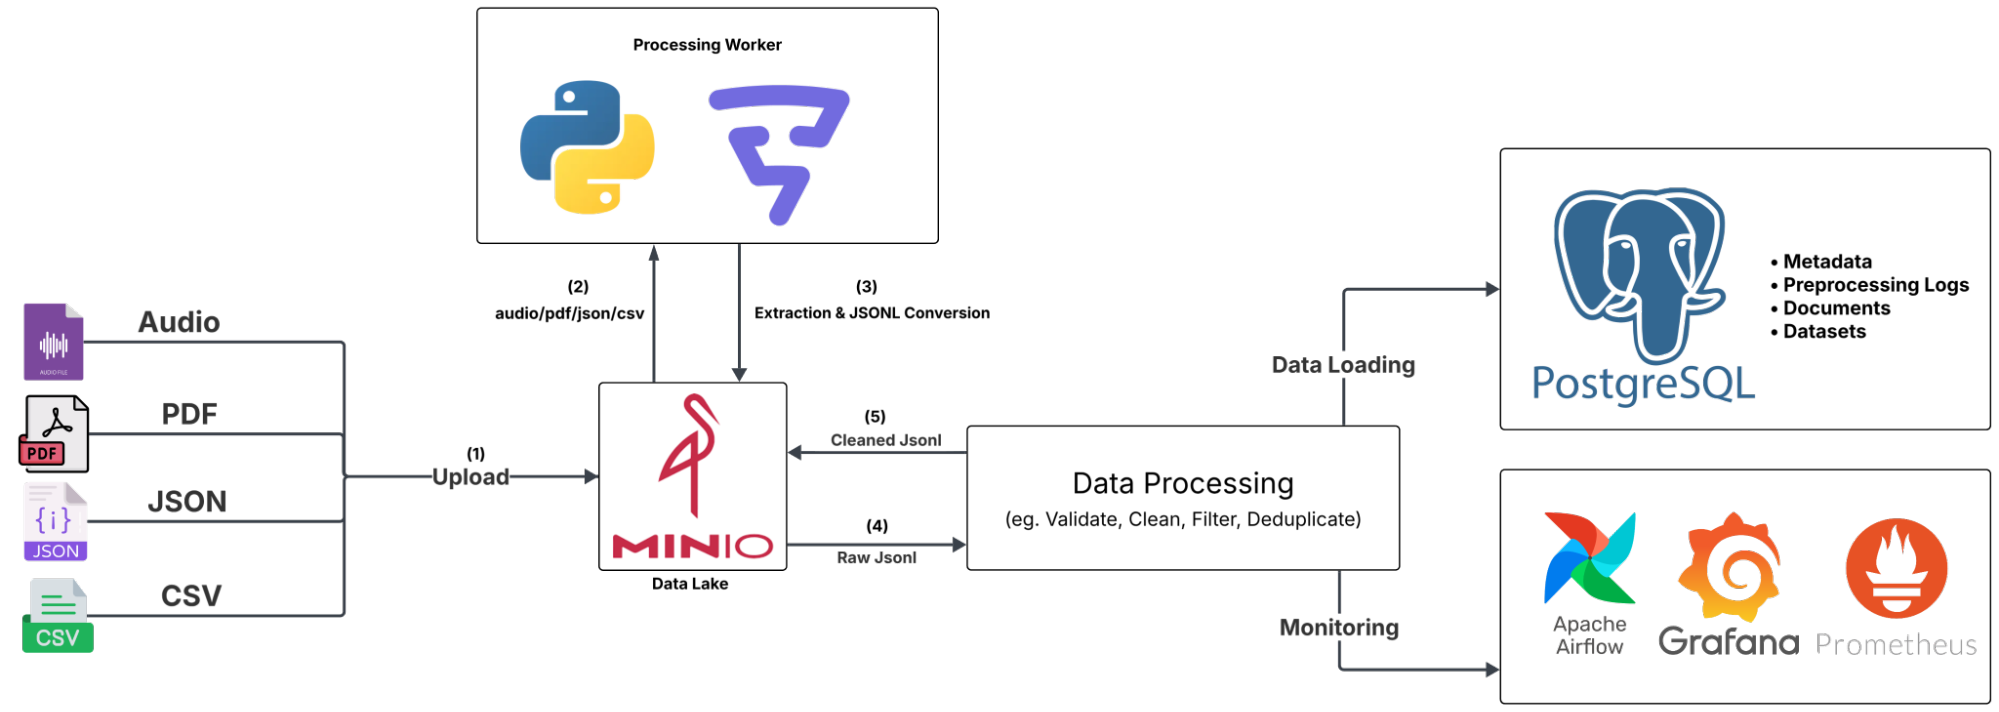
\includegraphics[width=0.9\textwidth]{figures/image1.png}
\caption{Automated Data Ingestion and Pipeline System Architecture}\label{fig:arch}
\end{figure}

As shown in Figure~\ref{fig:arch}, the architecture starts from the input layer, where users or data providers upload raw files into the system. The supported input formats include audio, PDF, JSON and CSV. These files are uploaded into MinIO, which acts as the main Data Lake of the system. MinIO is responsible for storing the original raw files as well as the cleaned outputs produced after processing. Using MinIO allows the system to organize data into different storage zones and maintain the separation between raw data and processed data.

\begin{figure}[H]\centering
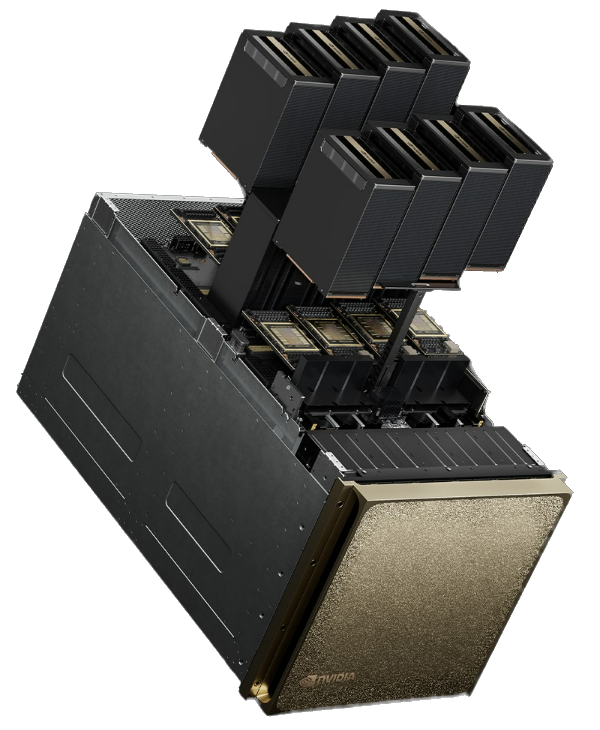
\includegraphics[width=0.4\textwidth]{figures/image21.png}
\caption{NVIDIA B200 GPUs}\label{fig:b200}
\end{figure}

After the raw files are uploaded into MinIO, the Processing Worker retrieves the input files for extraction and conversion. The Processing Worker is implemented using Python-based scripts and is orchestrated by Apache Airflow. Apache Airflow is used to manage the execution order of the pipeline tasks, schedule workflows, monitor task status and retry failed tasks when necessary.

\begin{figure}[H]\centering
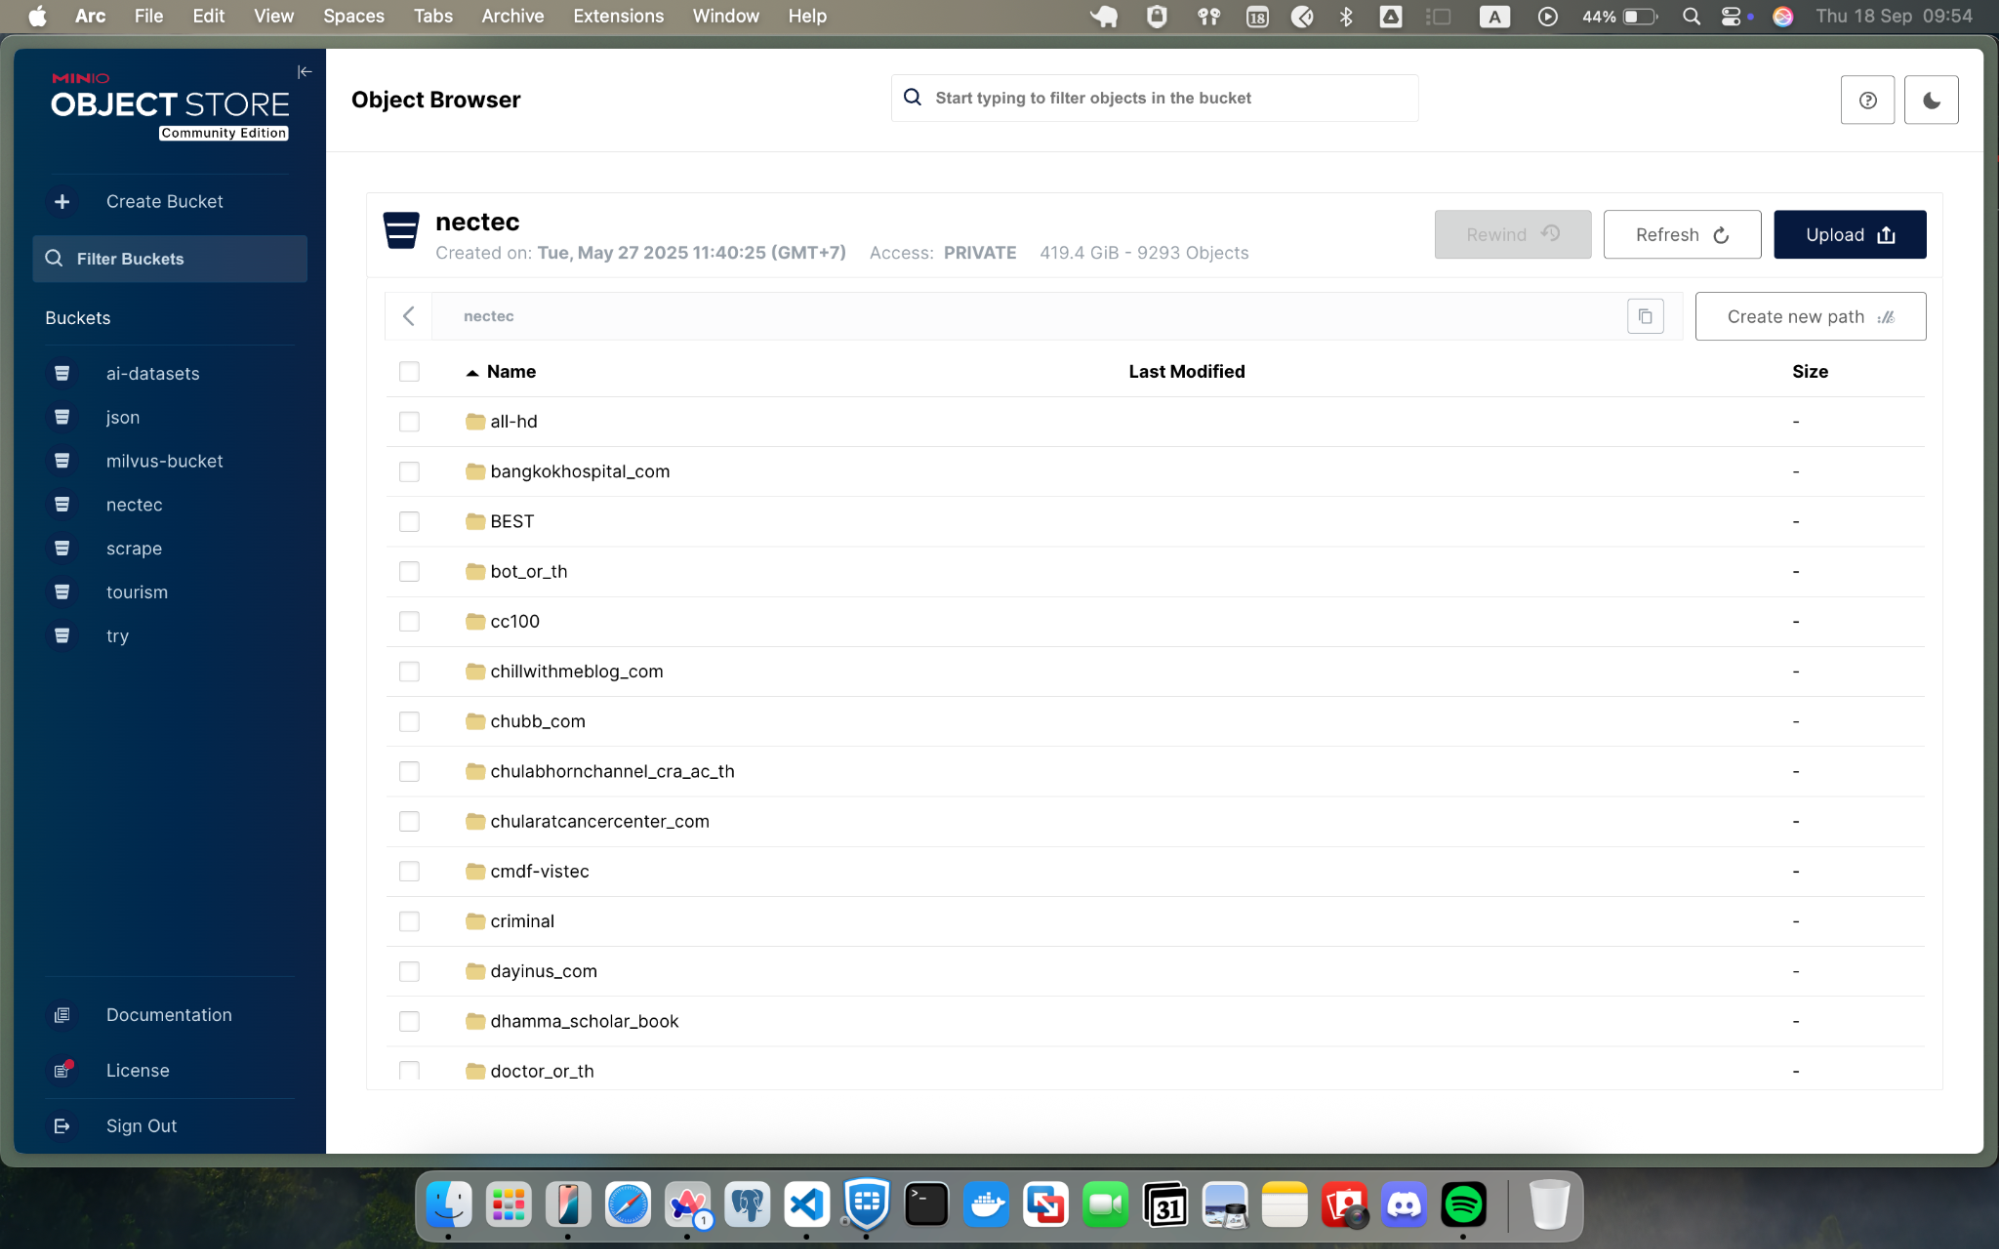
\includegraphics[width=0.9\textwidth]{figures/image22.png}
\caption{MinIO Object Storage (Data Lake Interface)}\label{fig:minio-iface}
\end{figure}

The Processing Worker performs different tasks depending on the input file type. For PDF files, the system extracts text from documents. If the PDF contains embedded text, the text can be extracted directly. If the PDF is image-based or scanned, the system applies OCR to convert the document image into machine-readable text. For audio files, the system applies an ASR model to convert speech into text. In this project, audio processing is supported by the company's GPU infrastructure using NVIDIA B200, which provides high computational performance for model inference tasks. For JSON and CSV files, the system reads the structured or semi-structured content and converts it into a common JSON-based format for further processing.

After extraction and conversion, the output from the Processing Worker is converted into raw JSON. This raw JSON acts as an intermediate representation of the extracted data and helps standardize different sources before they enter the data processing layer. The raw JSON is then passed to the Data Processing layer, which is responsible for improving the quality of the extracted data before it is stored as final output. The main operations in this layer include validation, cleaning, filtering and deduplication.

This processing layer is especially important for Thai-language datasets, which may include encoding issues, inconsistent spacing, missing tone marks or OCR/ASR errors. For PDF data, this may include removing low-quality OCR results or empty pages. For audio data, this may include filtering inaccurate transcripts or silent audio. For JSON and CSV data, this may include checking required fields, normalizing text and removing duplicate records. Once the data has passed the processing stage, the cleaned result is stored back into MinIO as cleaned JSONL.

\begin{figure}[H]\centering
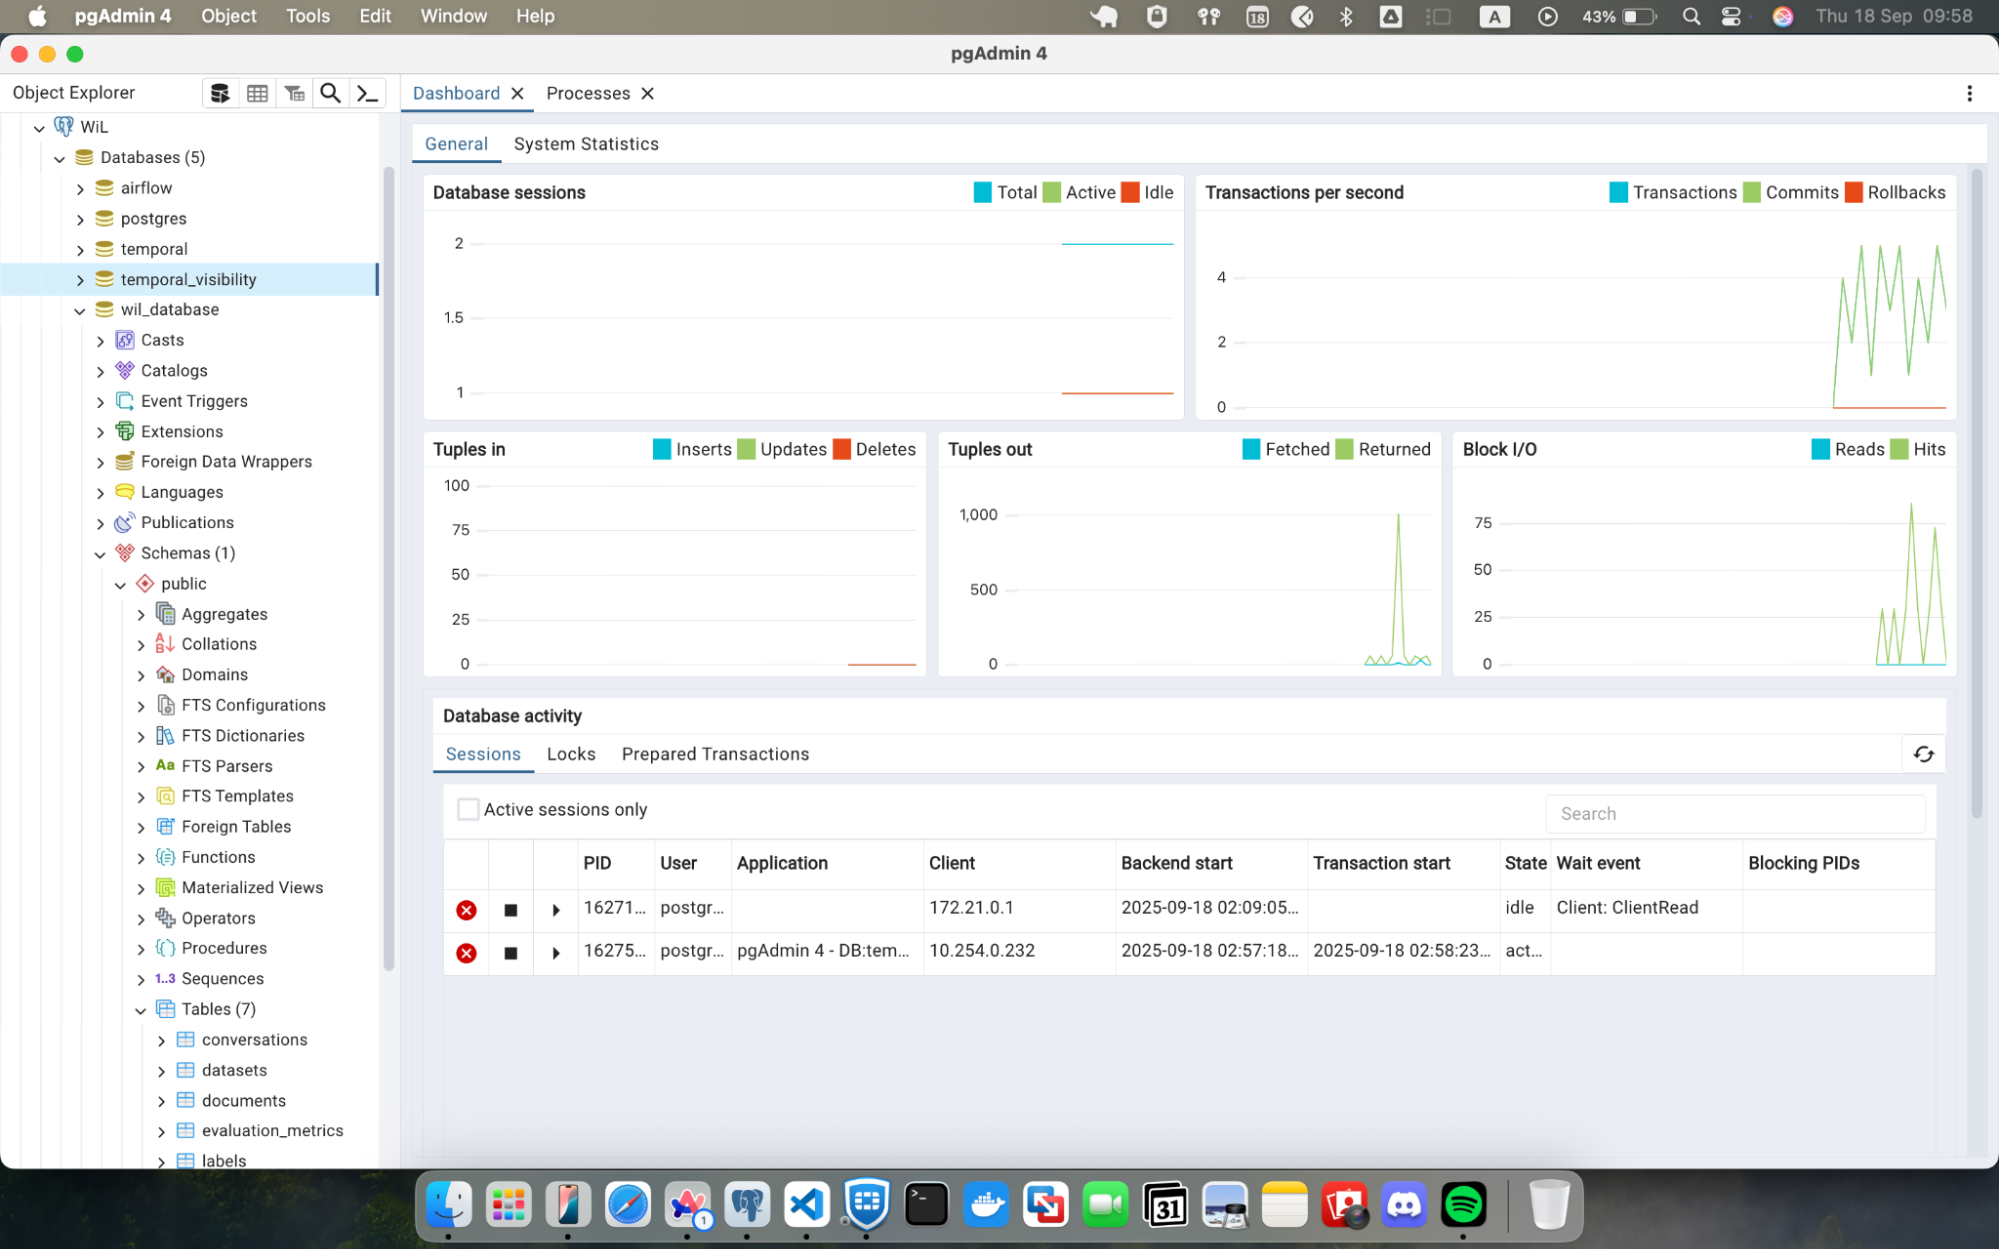
\includegraphics[width=0.9\textwidth]{figures/image17.png}
\caption{pgAdmin 4 Interface for PostgreSQL Data Warehouse}\label{fig:pgadmin}
\end{figure}

In addition to storing cleaned outputs in MinIO, the system also loads important information into PostgreSQL. PostgreSQL acts as the main database for structured storage, querying and metadata management. The database stores key information such as datasets, documents, preprocessing logs and metadata. The connection between the data processing layer and PostgreSQL is important because AI-ready datasets should not only contain cleaned text but also processing history and metadata.

\begin{figure}[H]\centering
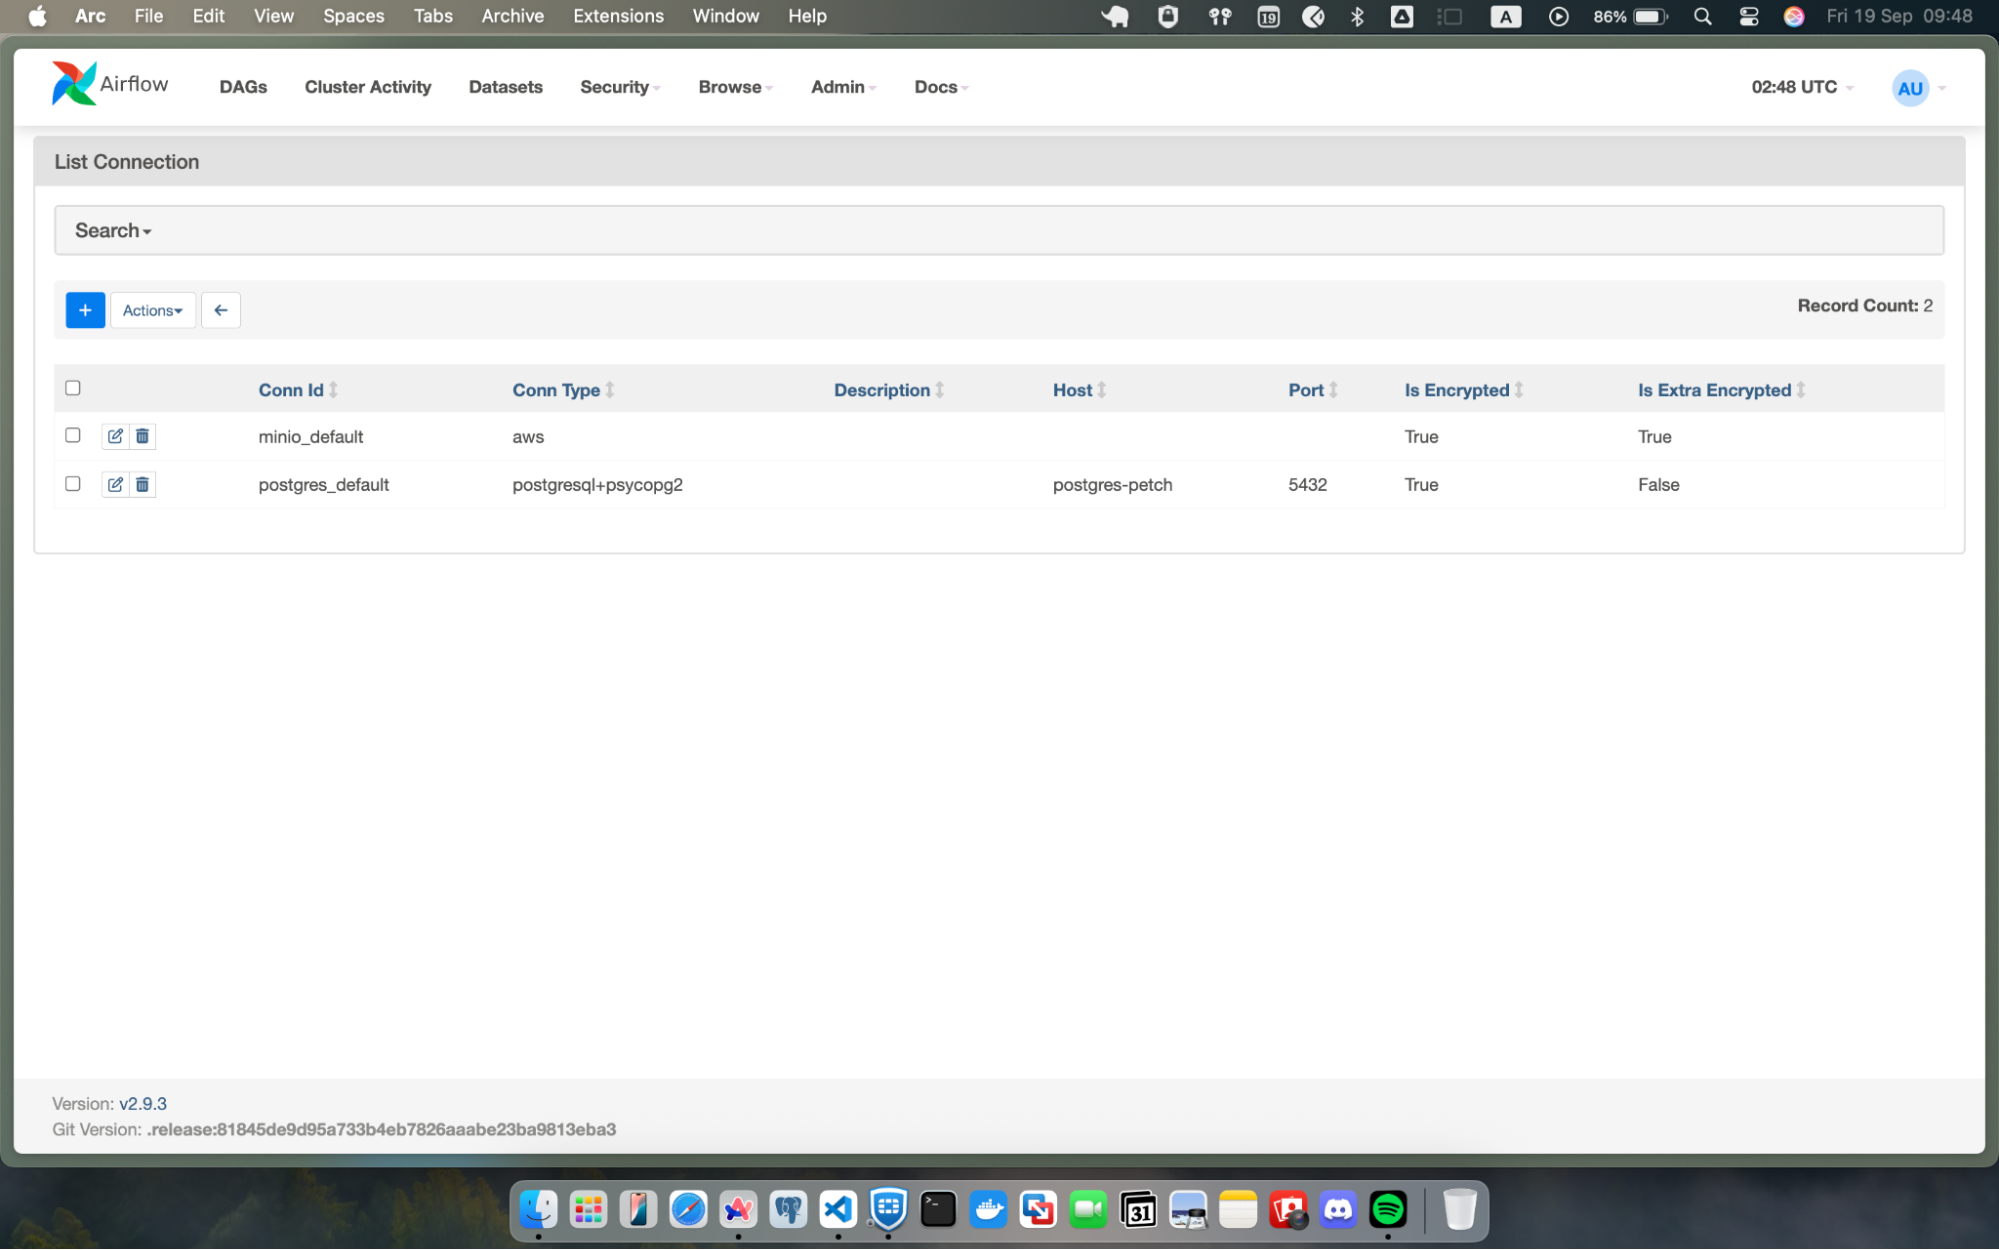
\includegraphics[width=0.9\textwidth]{figures/image26.png}
\caption{Apache Airflow Interface for Data Pipeline Connection}\label{fig:airflow-iface}
\end{figure}
\newpage
The final part of the architecture is the Monitoring layer. The system uses Apache Airflow, Grafana and Prometheus to monitor pipeline execution and system performance. Airflow provides task-level monitoring, while Prometheus collects metrics and Grafana visualizes them through dashboards. These monitoring tools help the development team track whether the pipeline is running correctly and identify problems such as failed tasks, slow processing, high resource usage or abnormal data volume.

Overall, the updated architecture follows a clear end-to-end flow: raw input files are uploaded into MinIO; the Processing Worker extracts and converts the files into raw JSON; the Data Processing layer validates, cleans, filters and removes duplicates; the cleaned JSONL output is stored back into MinIO; metadata is loaded into PostgreSQL; and Airflow, Prometheus and Grafana are used to monitor pipeline execution and system health. This design focuses on practical batch-based data ingestion and preparation rather than real-time streaming.

%%%%%%%%%%%%%%%%%%%%%%%%%%%%%%%%%%%%%%%%%%%%%%%%%%%%%%%%%%%%%%
%%%%%%%%%%%%%%%  CHAPTER 3  %%%%%%%%%%%%%%%%%%%%%%%%%%%%%%%%%%
%%%%%%%%%%%%%%%%%%%%%%%%%%%%%%%%%%%%%%%%%%%%%%%%%%%%%%%%%%%%%%
\chapter{Methodology and Designs}

\section{Introduction}

This chapter presents the current progress of methodology and system design for the development of the Automated Data Ingestion and Pipeline System for AI Model Training. The methodology is grounded in industry-proven data engineering principles and aligns with the project scope, requirements and metadata schema. This chapter details the functional requirements, the overall architecture, the containerized service design, data lake and data warehouse structures, the entire pipeline orchestration mechanisms, and the monitoring framework used to ensure reliability and scalability.

\section{Functional Requirements}

The functional requirements were derived from the system objectives, the dataset schema and the expected output formats for AI model training. These requirements define what the system must accomplish to support fully automated data ingestion and preparation.

\subsection{Data Ingestion Requirements}
The system is capable of ingesting the following data types:
\begin{itemize}
\item Structured data: CSV, SQL, JSON, JSONL
\item Unstructured data: raw text, scanned PDFs, images and audio
\end{itemize}

\subsection{Data Cleaning and Transformation Requirements}
\begin{itemize}
\item Perform encoding normalization, whitespace and punctuation cleaning and structural standardization.
\item Remove duplicate data based on checksums as defined in the metadata schema.
\item Apply Thai-specific preprocessing rules including Thai-character ratio filtering required for NECTEC corpora.
\item Normalize and flatten formats into standardized JSONL or Parquet representations.
\item Extract text from PDF and image data using an OCR engine optimized for Thai language.
\item Extract text from audio files using an ASR engine optimized for Thai language.
\end{itemize}

\subsection{Output and Storage Requirements}
\begin{itemize}
\item Cleaned intermediate data in a clean zone.
\item Final AI-ready datasets in processed zones using formats such as JSONL, Parquet and TFRecords.
\item Metadata stored in a relational warehouse, following the provided schema definitions.
\end{itemize}

\subsection{Orchestration and Monitoring Requirements}
\begin{itemize}
\item Automate all ingestion, cleaning, OCR and ASR workflows through Apache Airflow DAGs.
\item Provide traceability and fault tolerance through logging, retries and status tracking.
\item Incorporate Prometheus and Grafana for system-level monitoring as required in the architecture plan.
\end{itemize}
\newpage
\section{System Design}

\subsection{Architectural Overview}
The system follows a modular Data Lakehouse architecture composed of:
\begin{itemize}
\item A Data Lake (MinIO) for storing raw, cleaned and processed files.
\item A Data Warehouse (PostgreSQL) for metadata management and querying.
\item An Orchestration Layer (Apache Airflow) for pipeline automation.
\item Python-based preprocessing modules for structured, semi-structured and unstructured data.
\item Monitoring services (Prometheus, Grafana) for system observability.
\end{itemize}

\subsection{Containerized Service Architecture}
All system components are deployed using the company's platform to ensure reproducibility, isolation and consistent execution across environments. Each service plays a specific role within the overall pipeline:
\begin{itemize}
\item \textbf{MinIO} (\texttt{minio/minio:latest}) serves as the Data Lake for all raw, cleaned and processed data. Its S3-compatible API supports seamless integration with Python scripts, Airflow tasks and machine learning frameworks.
\item \textbf{PostgreSQL} (\texttt{postgres:13}) implements the Data Warehouse using the metadata schema.
\item \textbf{Airflow} Webserver, Scheduler and Init (\texttt{apache/airflow:3.1.0}) implement DAGs.
\item \textbf{pgAdmin} (\texttt{dpage/pgadmin4}) provides administrative access to the metadata warehouse.
\item \textbf{Prometheus} (\texttt{prom/prometheus}) collects metrics from exporters (Airflow, PostgreSQL, MinIO) and stores them as time-series data.
\item \textbf{Grafana} (\texttt{grafana/grafana}) reads metrics from Prometheus and provides dashboards.
\item \textbf{PostgreSQL Exporter} (\texttt{prometheuscommunity/postgres-exporter:latest}) exposes database metrics to Prometheus.
\item \textbf{StatsD Exporter} (\texttt{prom/statsd-exporter:v0.26.0}) receives StatsD metrics from Airflow.
\end{itemize}

\section{Data Lake Structure}

\begin{figure}[H]\centering
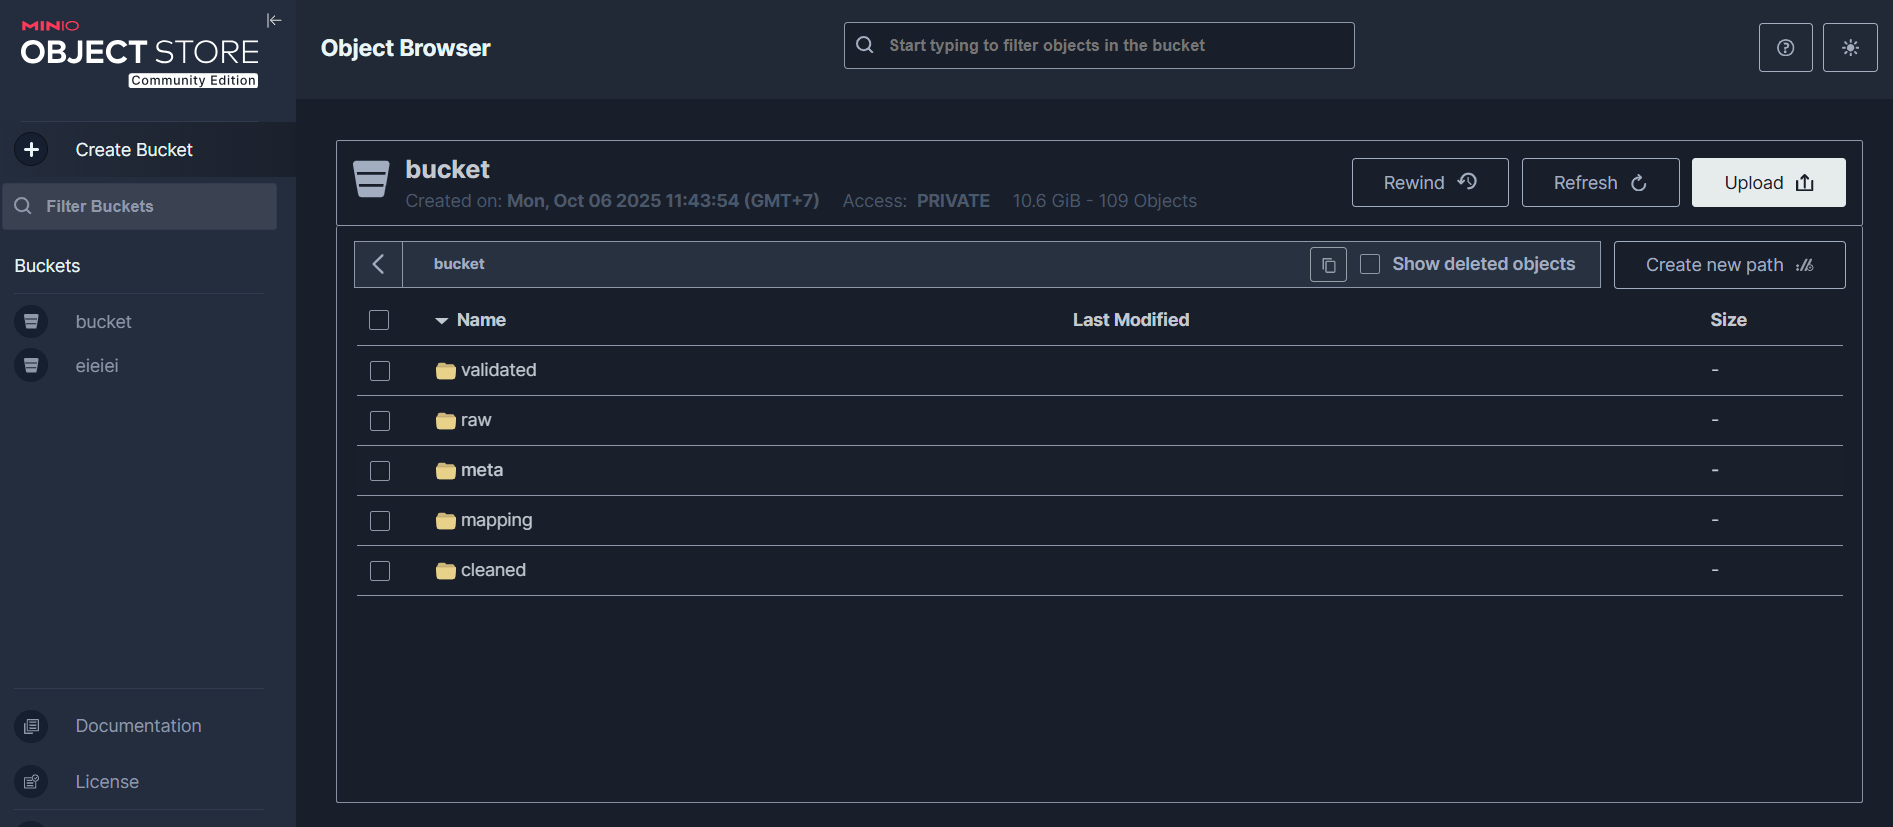
\includegraphics[width=0.9\textwidth]{figures/image30.png}
\caption{MinIO Interface}\label{fig:minio-buckets}
\end{figure}
\newpage
\subsection{MinIO Structure}
MinIO is used as the object storage layer for all datasets in the pipeline. A main bucket is created and organized into logical prefixes that follow the processing steps of the pipeline: \texttt{raw}, \texttt{cleaned}, \texttt{validated}, \texttt{meta} and \texttt{mapping}. The \texttt{raw} prefix stores files exactly as they are received from the original sources. The \texttt{cleaned} prefix contains the output of the text cleaning scripts, while the \texttt{validated} prefix stores only the files that pass schema and data-quality checks and are ready to be used for model training or downstream analytics. The \texttt{meta} prefix is used to store log files from each processing step. The \texttt{mapping} prefix stores the outputs from an additional mapping step required for some NECTEC datasets, in which raw files are joined with CSV mapping files provided by NECTEC and saved for later ingestion into the database. This folder structure makes it clear which stage each file belongs to and supports a simple, traceable flow from raw data to validated data.

\subsection{Bucket Versioning and Replication}
Bucket versioning is enabled for the main bucket so that previous versions of objects are kept when files are updated or overwritten during pipeline re-runs. This helps protect against accidental data loss and allows the system to roll back to an earlier version of a file if needed. In addition, lifecycle rules are configured to automatically clean up old object versions and temporary files after a retention period, which prevents unlimited growth of storage usage. MinIO bucket replication is also configured so that objects written to the main bucket are asynchronously copied to a second bucket on another MinIO deployment. This replication provides an additional backup of the cleaned and validated data and improves the resilience of the overall system.

\section{Data Warehouse}

\begin{figure}[H]\centering
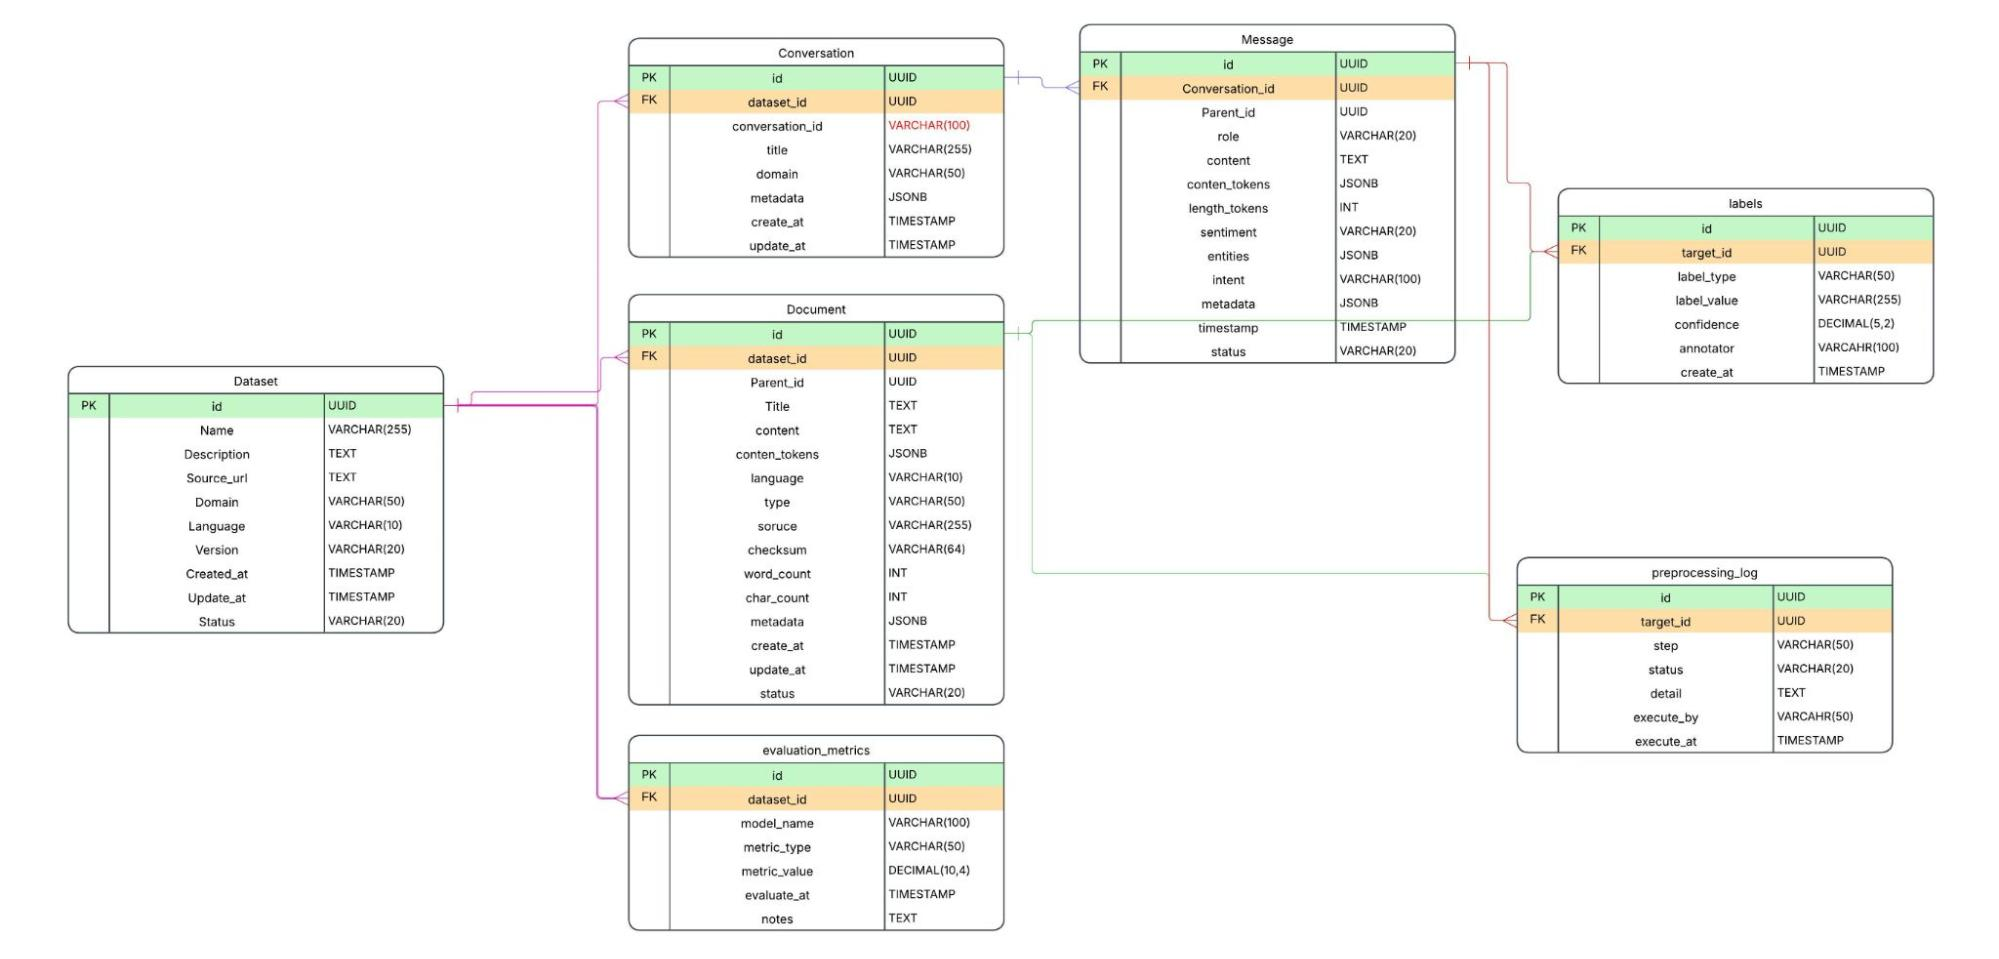
\includegraphics[width=0.95\textwidth]{figures/image14.jpg}
\caption{Database schema for PostgreSQL}\label{fig:db-schema}
\end{figure}

The data warehouse uses PostgreSQL as a central database for managing dataset metadata, documents, labels and processing logs. The schema is designed around a small set of core tables with UUID primary keys and foreign-key links between them.

\begin{table}[H]
\centering
\caption{\texttt{datasets} table schema}\label{tbl:db-datasets}
\begin{tabular}{|p{0.22\textwidth}|p{0.18\textwidth}|p{0.45\textwidth}|}
\hline
\textbf{Field name} & \textbf{Type} & \textbf{Description} \\ \hline
id & UUID / BIGINT & Primary key \\ \hline
name & VARCHAR(255) & Dataset name \\ \hline
description & TEXT & Dataset details \\ \hline
source\_url & TEXT & Source URL or repository \\ \hline
domain & VARCHAR(50) & Categories such as general, medical, legal, tourism \\ \hline
language & VARCHAR(10) & Main languages of the dataset \\ \hline
version & VARCHAR(20) & Dataset version \\ \hline
created\_at & TIMESTAMP & Creation date \\ \hline
updated\_at & TIMESTAMP & Last edit date \\ \hline
status & VARCHAR(20) & raw, preprocessed, validated \\ \hline
\end{tabular}
\end{table}

\begin{table}[H]
\centering
\caption{\texttt{documents} table schema}\label{tbl:db-documents}
\begin{tabular}{|p{0.22\textwidth}|p{0.18\textwidth}|p{0.45\textwidth}|}
\hline
\textbf{Field name} & \textbf{Type} & \textbf{Description} \\ \hline
id & UUID / BIGINT & Primary key \\ \hline
dataset\_id & UUID & Foreign key $\rightarrow$ datasets.id \\ \hline
parent\_id & UUID & Reference to main document if sub-document \\ \hline
title & VARCHAR(255) & Topic / filename \\ \hline
content & TEXT & All content \\ \hline
content\_tokens & JSONB & Tokenized version (optional) \\ \hline
language & VARCHAR(10) & th, en, cn, etc. \\ \hline
type & VARCHAR(50) & paragraph, code, conversation, qa \\ \hline
source & VARCHAR(255) & Source \\ \hline
checksum & VARCHAR(64) & Hash of content to prevent duplicates \\ \hline
word\_count & INT & Word count \\ \hline
char\_count & INT & Character count \\ \hline
metadata & JSONB & Topic, domain, difficulty \\ \hline
created\_at & TIMESTAMP & Creation date \\ \hline
updated\_at & TIMESTAMP & Last edit date \\ \hline
status & VARCHAR(20) & raw, cleaned, validated \\ \hline
\end{tabular}
\end{table}

\begin{table}[H]
\centering
\caption{\texttt{conversations} table schema}\label{tbl:db-conversations}
\begin{tabular}{|p{0.22\textwidth}|p{0.18\textwidth}|p{0.45\textwidth}|}
\hline
\textbf{Field name} & \textbf{Type} & \textbf{Description} \\ \hline
id & UUID & Primary key \\ \hline
dataset\_id & UUID & Foreign key $\rightarrow$ datasets.id \\ \hline
conversation\_id & VARCHAR(100) & Identifier of conversation group \\ \hline
title & VARCHAR(255) & Name or topic of conversation \\ \hline
domain & VARCHAR(50) & Category, e.g., customer\_service, qa \\ \hline
metadata & JSONB & e.g., intent, scenario \\ \hline
created\_at & TIMESTAMP & Creation date \\ \hline
updated\_at & TIMESTAMP & Last edit date \\ \hline
\end{tabular}
\end{table}

\begin{table}[H]
\centering
\caption{\texttt{messages} table schema}\label{tbl:db-messages}
\begin{tabular}{|p{0.22\textwidth}|p{0.18\textwidth}|p{0.45\textwidth}|}
\hline
\textbf{Field name} & \textbf{Type} & \textbf{Description} \\ \hline
id & UUID & Primary key \\ \hline
conversation\_id & UUID & Foreign key $\rightarrow$ conversations.id \\ \hline
parent\_message & UUID & Reference to main topic if reply \\ \hline
role & VARCHAR(20) & user, assistant, system, moderator \\ \hline
content & TEXT & Information \\ \hline
content\_tokens & JSONB & Tokenized version \\ \hline
length\_tokens & INT & Token count \\ \hline
sentiment & VARCHAR(20) & e.g., positive, negative, neutral \\ \hline
entities & JSONB & e.g., \{"name": xyz\} \\ \hline
intent & VARCHAR(100) & Optional for fine-tuning \\ \hline
metadata & JSONB & Additional info, e.g., topic, urgency \\ \hline
timestamp & TIMESTAMP & Created message \\ \hline
status & VARCHAR(20) & raw, cleaned, validated \\ \hline
\end{tabular}
\end{table}

\begin{table}[H]
\centering
\caption{\texttt{labels} table schema}\label{tbl:db-labels}
\begin{tabular}{|p{0.22\textwidth}|p{0.18\textwidth}|p{0.45\textwidth}|}
\hline
\textbf{Field name} & \textbf{Type} & \textbf{Description} \\ \hline
id & UUID & Primary key \\ \hline
target\_id & UUID & Foreign key $\rightarrow$ messages.id or documents.id \\ \hline
label\_type & VARCHAR(50) & e.g., intent, topic, sentiment, category \\ \hline
label\_value & VARCHAR(255) & Label value, e.g., greeting, legal, positive \\ \hline
confidence & DECIMAL(5,2) & Confidence score (0--100\%) \\ \hline
annotator & VARCHAR(100) & User or AI model that created the label \\ \hline
created\_at & TIMESTAMP & Creation date \\ \hline
\end{tabular}
\end{table}

\begin{table}[H]
\centering
\caption{\texttt{preprocessing\_logs} table schema}\label{tbl:db-prep-logs}
\begin{tabular}{|p{0.22\textwidth}|p{0.18\textwidth}|p{0.45\textwidth}|}
\hline
\textbf{Field name} & \textbf{Type} & \textbf{Description} \\ \hline
id & UUID & Primary key \\ \hline
target\_id & UUID & Foreign key $\rightarrow$ documents.id or messages.id \\ \hline
step & VARCHAR(50) & e.g., remove\_html, normalize\_unicode, tokenize \\ \hline
status & VARCHAR(20) & success, failed \\ \hline
details & TEXT & Result info, e.g., error message \\ \hline
executed\_by & VARCHAR(50) & Script or user \\ \hline
executed\_at & TIMESTAMP & Processed time \\ \hline
\end{tabular}
\end{table}

\begin{table}[H]
\centering
\caption{\texttt{evaluation\_metrics} table schema}\label{tbl:db-eval}
\begin{tabular}{|p{0.22\textwidth}|p{0.18\textwidth}|p{0.45\textwidth}|}
\hline
\textbf{Field name} & \textbf{Type} & \textbf{Description} \\ \hline
id & UUID & Primary key \\ \hline
dataset\_id & UUID & Foreign key $\rightarrow$ datasets.id \\ \hline
model\_name & VARCHAR(100) & Model name \\ \hline
metric\_type & VARCHAR(50) & e.g., accuracy, bleu, rouge, perplexity \\ \hline
metric\_value & DECIMAL(10,4) & Metric value \\ \hline
evaluated\_at & TIMESTAMP & Evaluation date \\ \hline
notes & TEXT & More info, e.g., subset, conditions \\ \hline
\end{tabular}
\end{table}

\newpage
\textbf{Relationships:}
\begin{enumerate}
\item datasets $\rightarrow$ documents (1:N)
\item datasets $\rightarrow$ conversations (1:N)
\item conversations $\rightarrow$ messages (1:N)
\item documents/messages $\rightarrow$ labels (1:N)
\item documents/messages $\rightarrow$ preprocessing\_logs (1:N)
\end{enumerate}

The \texttt{datasets} table stores one record for each dataset used in the pipeline. The \texttt{documents} table stores individual text units that are ready to be used for analysis or model training. Each document row is linked to a dataset through \texttt{dataset\_id}. The \texttt{labels} table is a generic table for storing labels for any target record, allowing the system to attach many different kinds of labels to the same text without changing the main tables. The \texttt{preprocessing\_log} table stores detailed logs for each processing step applied to a given target.

\section{Orchestration}

\subsection{JSONL Pipeline}

The end-to-end JSONL pipeline is orchestrated using Apache Airflow in a DAG named \texttt{sensor\_demo}. This DAG is scheduled to run every hour and is designed to automatically detect new raw \texttt{.jsonl} files in MinIO, run the full preprocessing pipeline and update both the PostgreSQL database and the monitoring logs. Whenever new files appear in the configured MinIO prefix, Airflow picks them up and processes them without manual intervention.

\begin{figure}[H]\centering
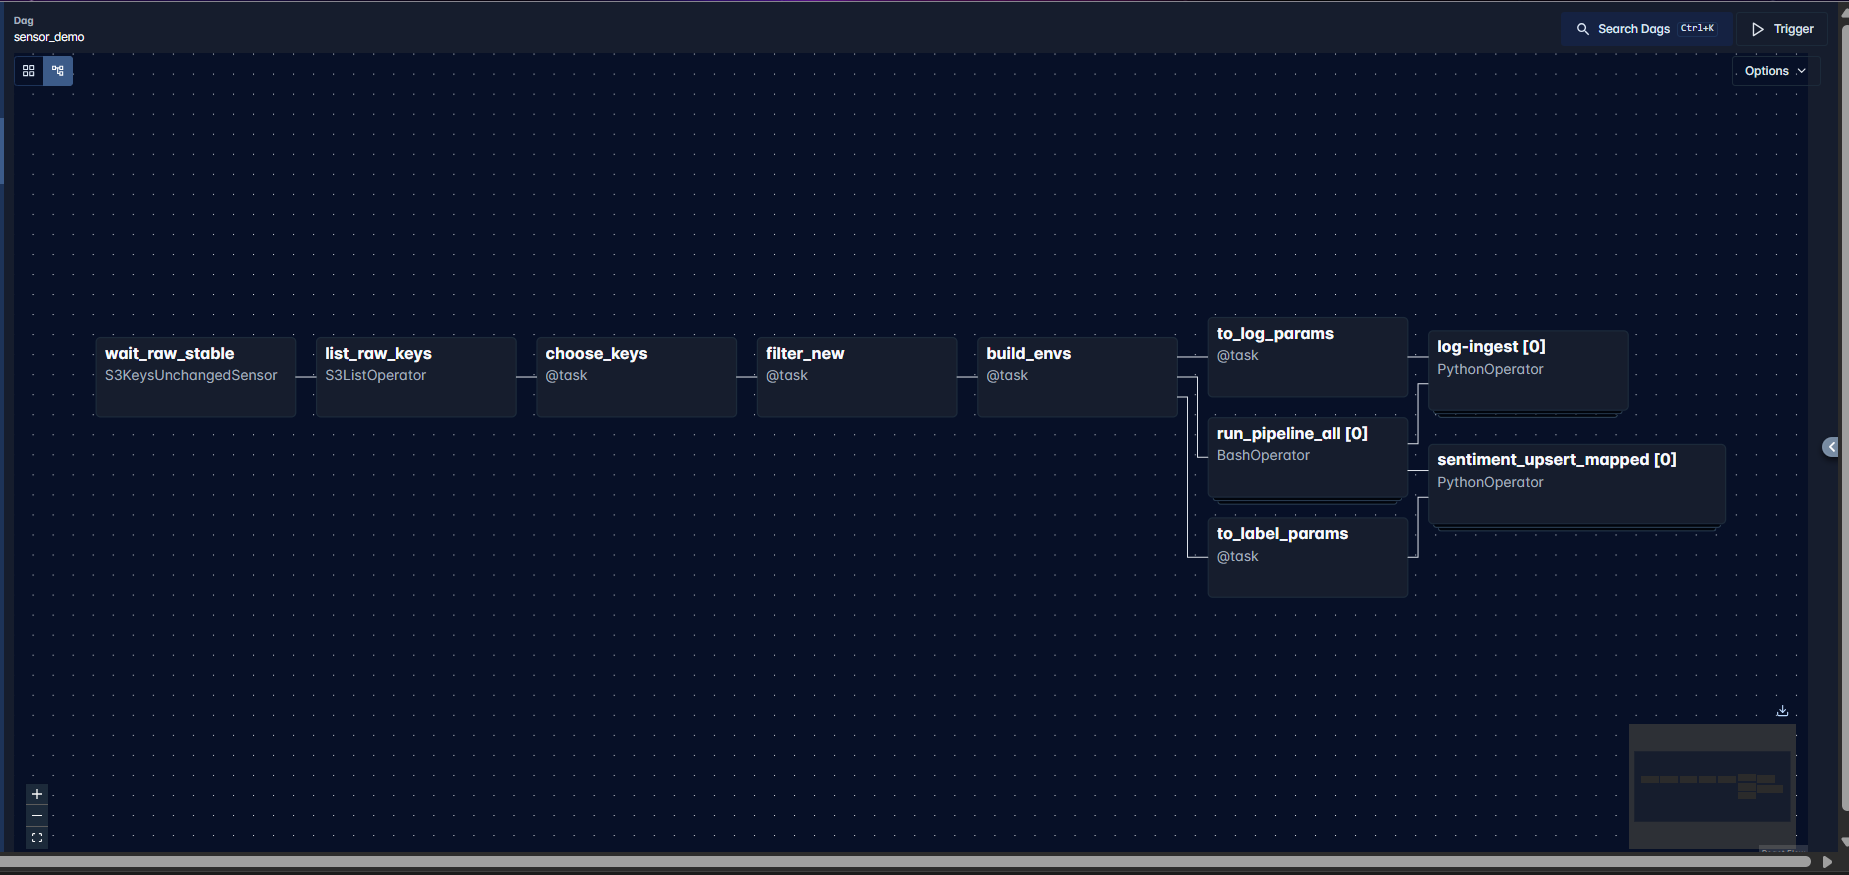
\includegraphics[width=0.95\textwidth]{figures/image3.png}
\caption{Apache Airflow graph view DAGs}\label{fig:airflow-graph}
\end{figure}

The first section of the DAG focuses on detecting new and stable input files. The task \texttt{wait\_raw\_stable} uses \texttt{S3KeysUnchangedSensor} to make sure that files in the \texttt{raw} prefix are no longer changing before starting the pipeline. After that, \texttt{list\_raw\_keys} uses \texttt{S3ListOperator} to list all raw object keys under the configured bucket and prefix. The next task, \texttt{choose\_keys}, is a Python \texttt{@task} that filters this list according to the dataset and directory structure. Then, \texttt{filter\_new} compares the selected keys with previously processed files and keeps only those that have not yet been ingested.

\begin{figure}[H]\centering
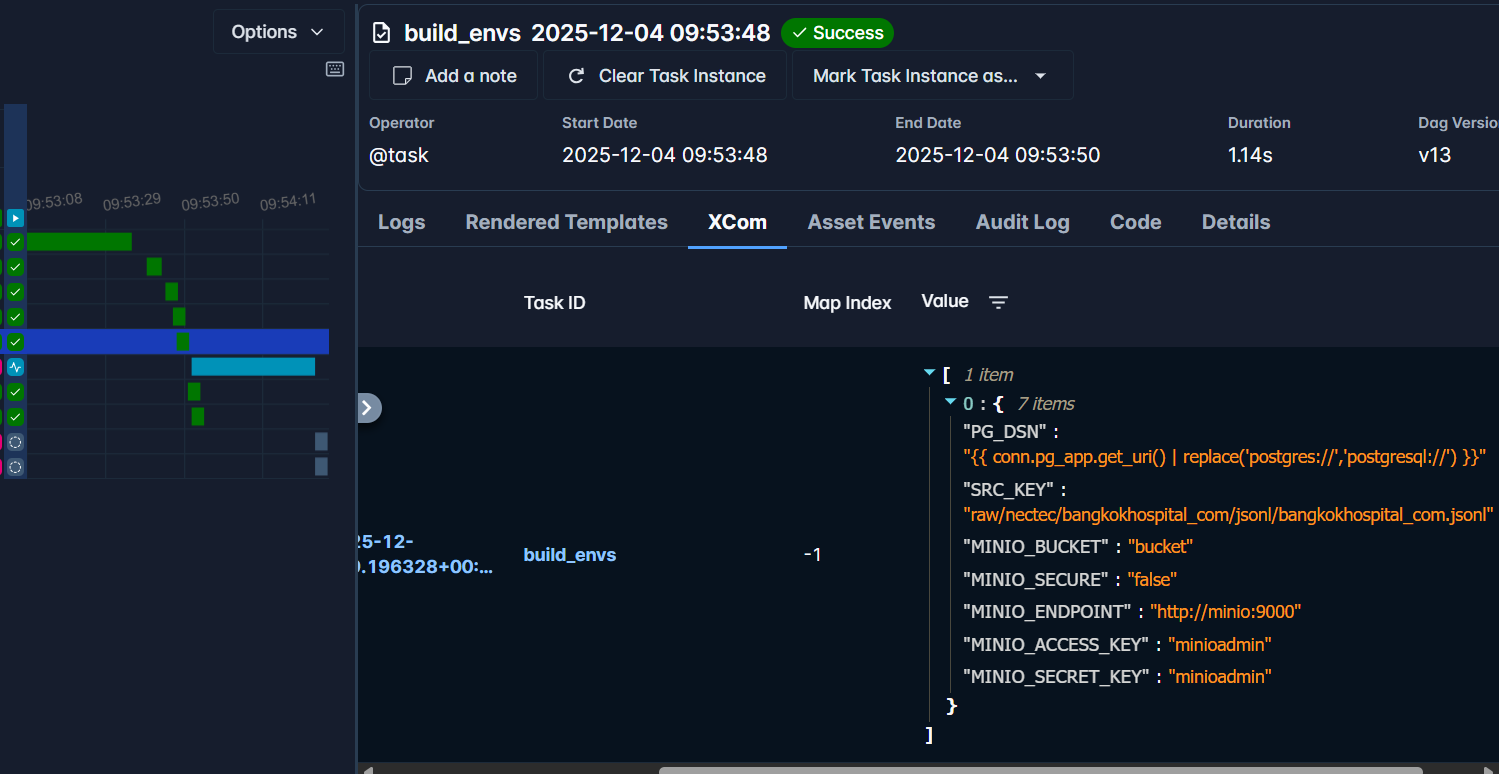
\includegraphics[width=0.9\textwidth]{figures/image6.png}
\caption{Apache Airflow Build environment task detail}\label{fig:airflow-buildenvs}
\end{figure}

Once the DAG has a list of new raw files, the \texttt{build\_envs} task prepares the runtime configuration for each file. This task constructs environment variables such as source key, dataset name, and various MinIO and database parameters required by the downstream scripts. The DAG then uses Airflow's dynamic task mapping to create one set of downstream tasks per input file.

After \texttt{build\_envs}, the pipeline splits into three parallel branches that handle ingestion, logging and labelling. The \texttt{run\_pipeline\_all} task is a \texttt{BashOperator} that calls the main \texttt{run.py} script for each file, which performs the core operations: reading the raw \texttt{.jsonl} from MinIO, cleaning and validating the text, running any required mapping step, writing the cleaned or mapped outputs back to MinIO, and inserting document records into the PostgreSQL \texttt{documents} table. In parallel with ingestion, the \texttt{to\_log\_params} task prepares log parameters for each processed file, and the \texttt{log-ingest} task writes a structured log entry into the \texttt{preprocessing\_log} table.

The third branch handles automatic labelling. The \texttt{to\_label\_params} task prepares the parameters required to call the Thai sentiment model. The \texttt{sentiment\_upsert\_mapped} task then runs a Python function that loads the documents, calls the sentiment model and upserts the results into the \texttt{labels} table.

\begin{figure}[H]\centering
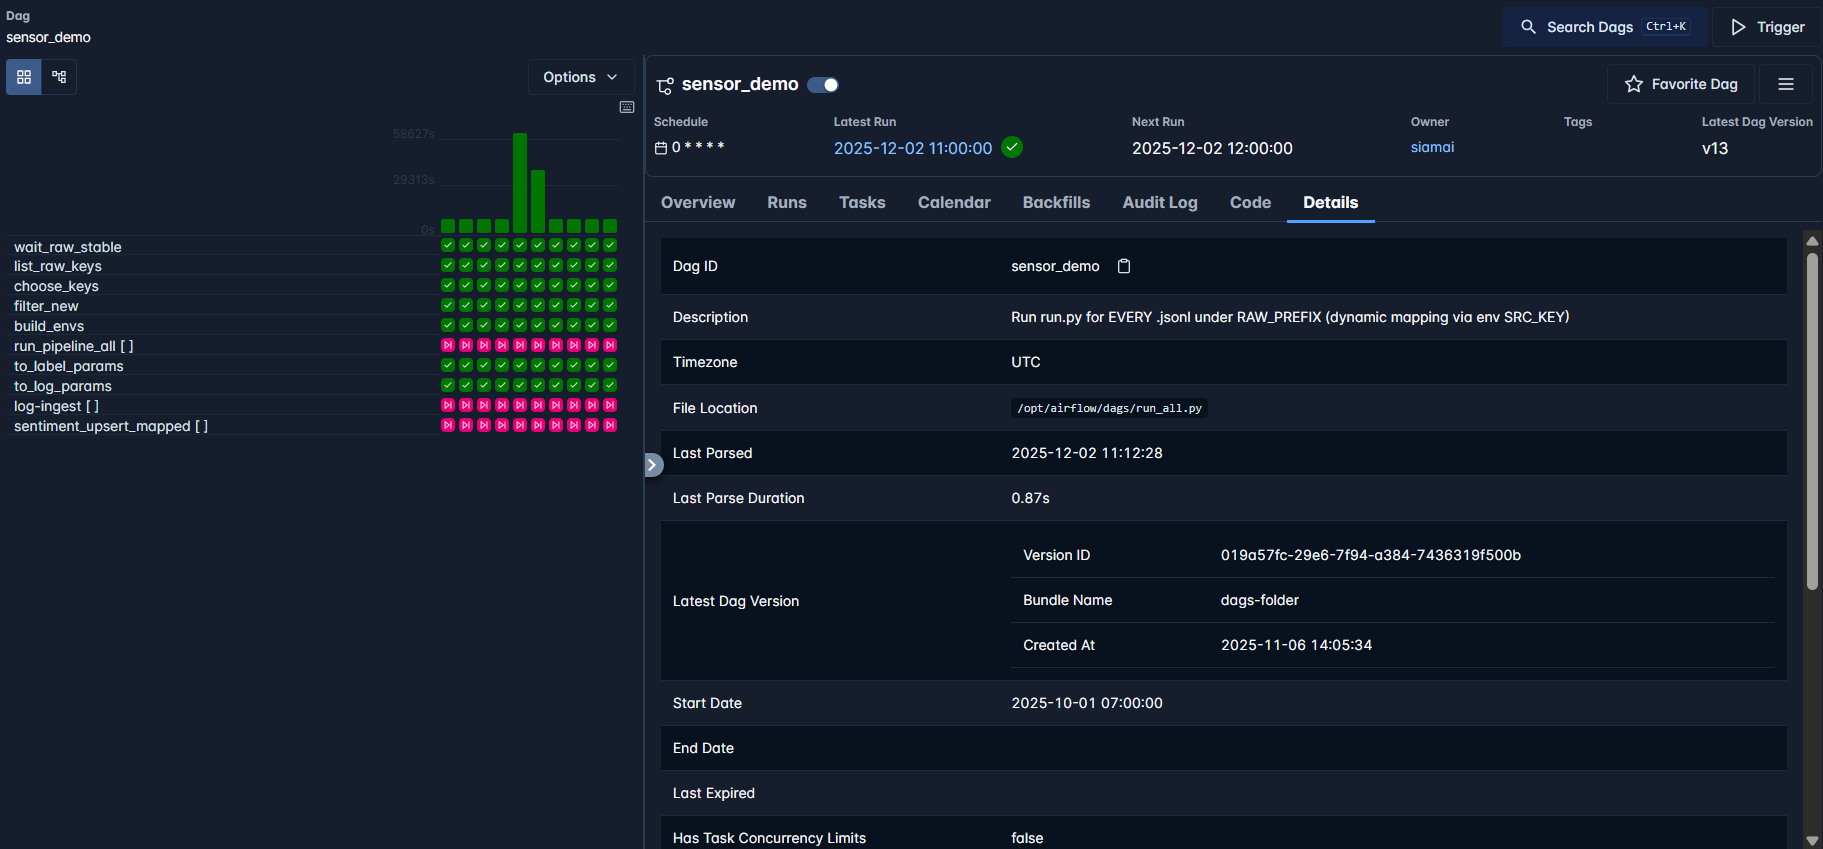
\includegraphics[width=0.95\textwidth]{figures/image2.png}
\caption{Apache Airflow Sensor\_demo DAG detail}\label{fig:airflow-sensor-demo}
\end{figure}

At the current stage, the \texttt{sensor\_demo} DAG is stable and has been executed many times, with most runs marked as successful. The DAG runs on a schedule and can also be triggered manually for testing. New raw files uploaded to the MinIO \texttt{raw/} prefix are correctly detected by the sensor, passed through the dynamic mapping pipeline and result in new \texttt{documents}, \texttt{labels} and \texttt{preprocessing\_log} records in PostgreSQL.

\subsection{Unstructured PDF OCR Pipeline}

The PDF OCR pipeline is orchestrated using Apache Airflow in a DAG named \texttt{pdf\_ocr\_pipeline}. This DAG is scheduled to run daily and is designed to automatically detect new PDF files in MinIO, run a hybrid text-extraction pipeline against them, and write both the clean text outputs and the per-page processing logs back to MinIO. Whenever new PDFs appear in the configured \texttt{raw/} prefix, or whenever a previous run produced documents marked as low-quality or failed, Airflow will pick them up and re-process them without manual intervention.

\begin{figure}[H]\centering
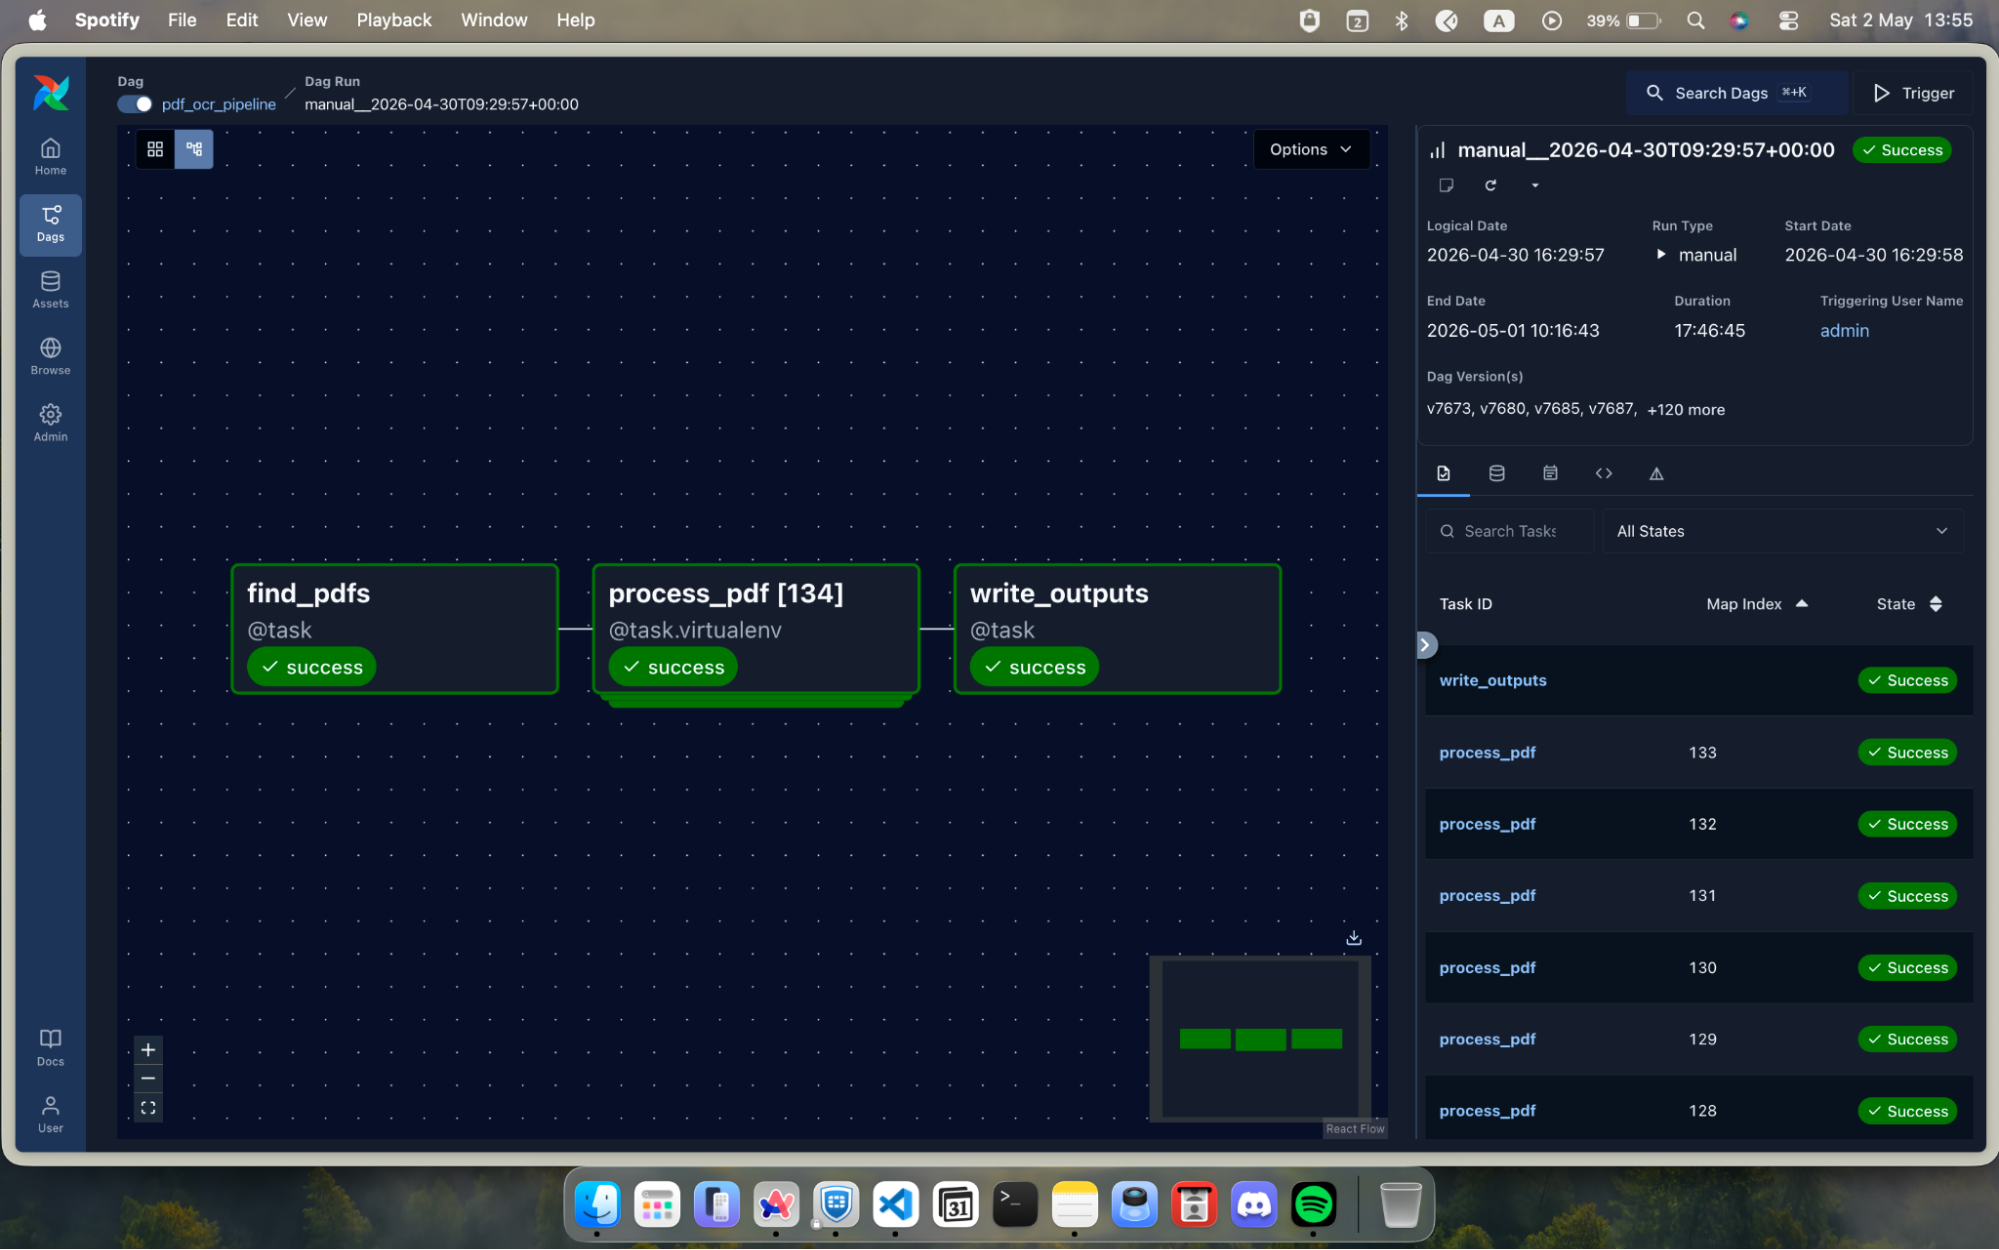
\includegraphics[width=0.95\textwidth]{figures/image29.png}
\caption{Apache Airflow graph view of \texttt{pdf\_ocr\_pipeline}}\label{fig:pdf-graph}
\end{figure}

The first section of the DAG focuses on discovering and filtering PDF files. The \texttt{find\_pdfs} task scans every bucket under the configured \texttt{raw/} prefix and lists all \texttt{.pdf} objects, while skipping any key that already sits under a \texttt{jsonl/} subdirectory. For each candidate file, the task reads the existing result and meta JSONL files in MinIO to check whether the PDF has already been processed successfully, or whether it previously ended in a \texttt{low\_quality}, \texttt{empty} or partially failed state. Documents that have already been processed cleanly are skipped, while those that failed or were flagged as low quality are re-queued for another attempt up to a configurable cap (\texttt{MAX\_RUN\_ATTEMPTS = 2}). This makes the pipeline idempotent and lets it recover gracefully from transient OCR-server failures across runs.

Once the list of PDFs is built, the DAG uses Airflow's dynamic task mapping to create one \texttt{process\_pdf} task instance per file. Each mapped task runs inside a cached virtual environment (\texttt{/tmp/pdf\_ocr\_venv}) that ships with all required libraries such as PyMuPDF, Pillow, NumPy, PyThaiNLP, requests and boto3, and is bound to a dedicated Airflow pool named \texttt{ocr\_pool} with a per-DAG-run concurrency limit of four. This configuration prevents the pipeline from overwhelming the upstream Typhoon-OCR service running on the B200 GPU.

\begin{figure}[H]\centering
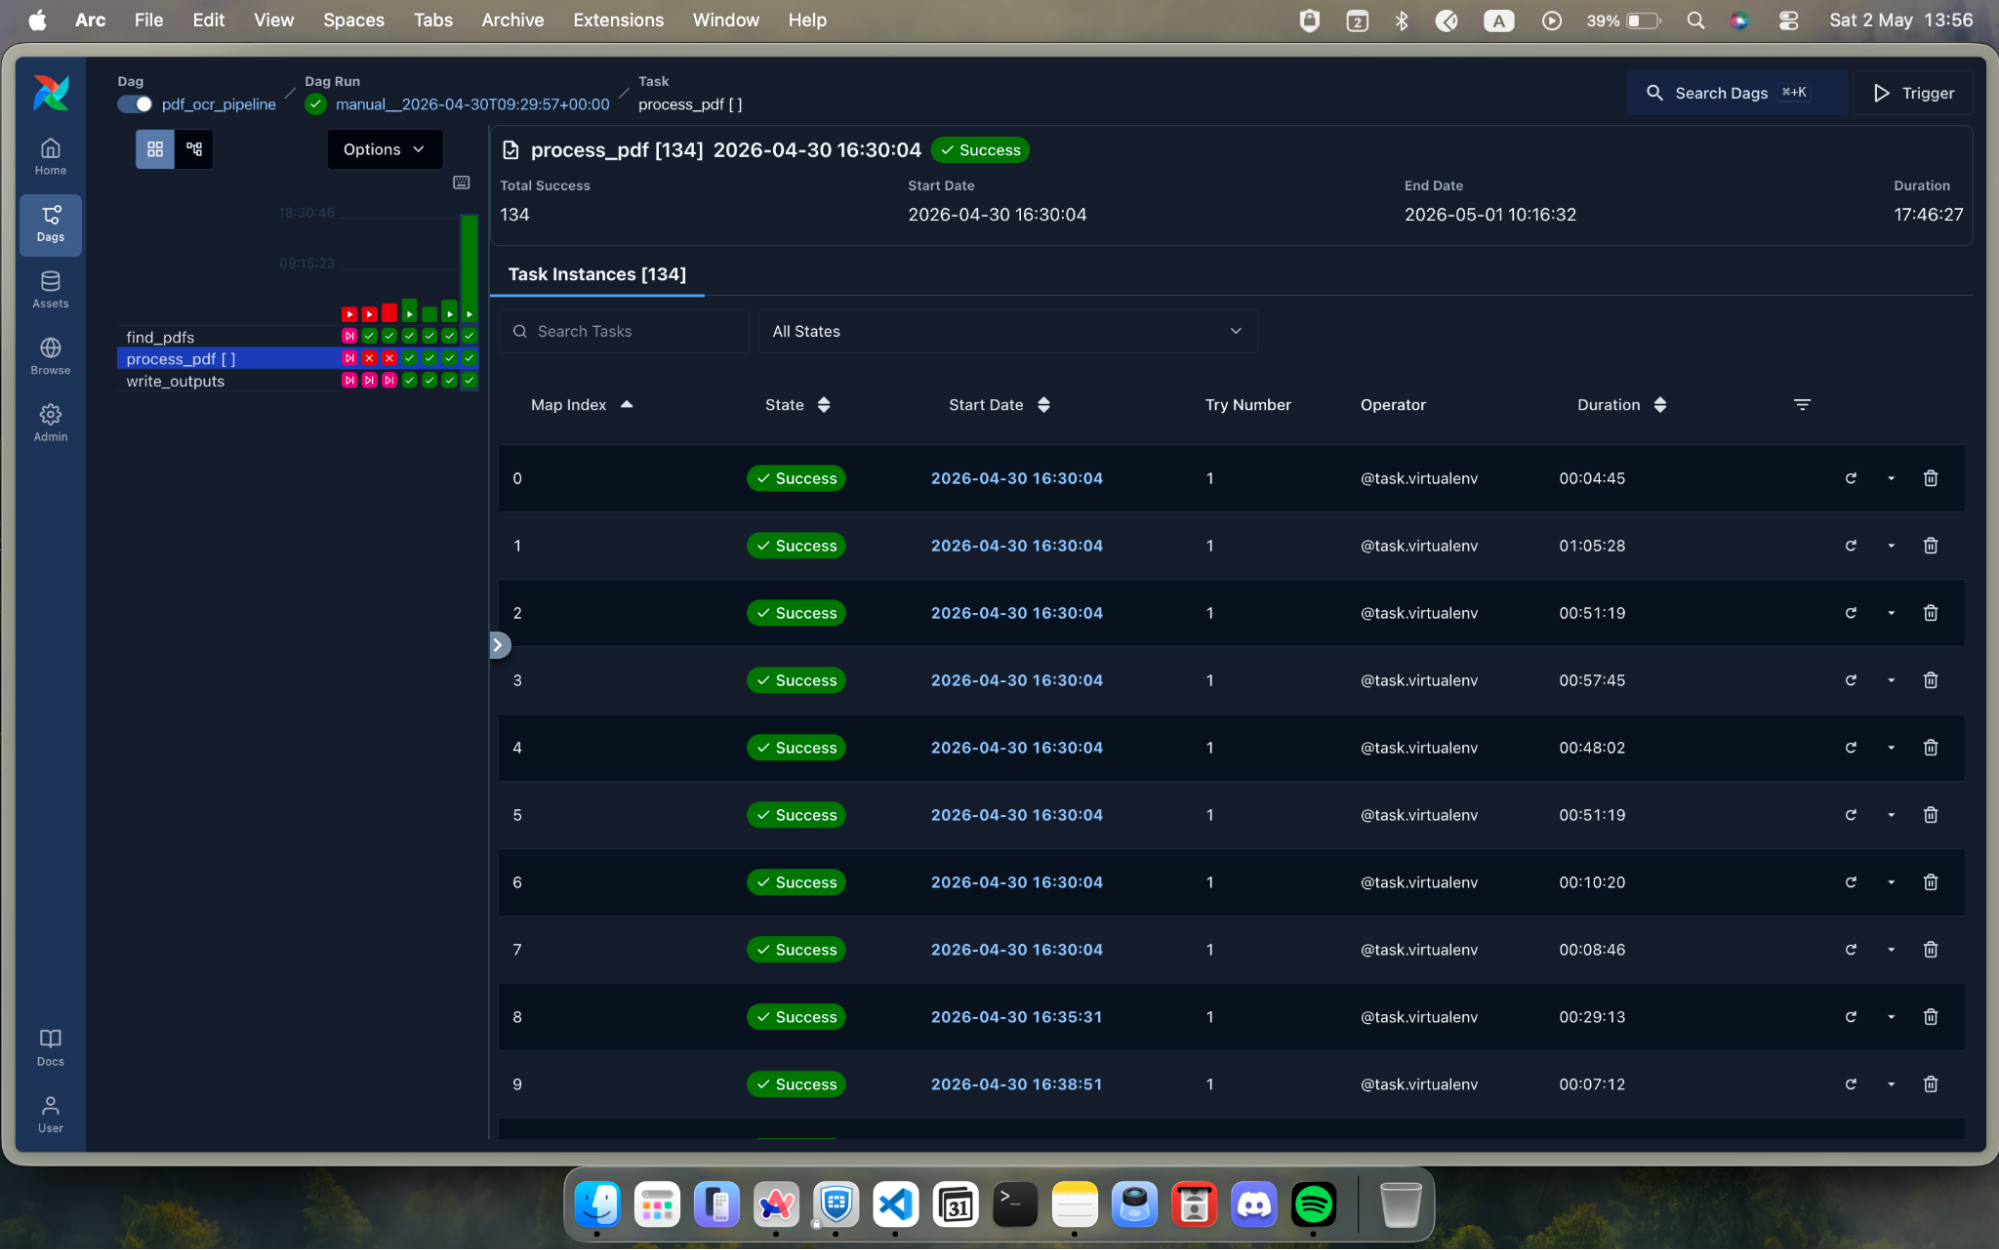
\includegraphics[width=0.9\textwidth]{figures/image33.png}
\caption{Apache Airflow \texttt{process\_pdf} task detail}\label{fig:pdf-process}
\end{figure}

Inside each \texttt{process\_pdf} task, the file is downloaded from MinIO and opened with PyMuPDF. The pipeline first attempts native text extraction at the page level: if a page yields enough characters of valid Thai text and shows no signs of font-encoding failure (such as \texttt{(cid:N)} glyphs, replacement characters or unmapped private-use-area codepoints), its text is kept and the page is recorded as having been handled by the PyMuPDF method. Pages that fail this check are routed to the OCR fallback path. Before invoking the OCR server, the task performs a health check; if the server is reachable, each remaining page is rendered to an RGB image at the configured DPI cascade (400 DPI primary, 300 DPI fallback when the JPEG exceeds the size limit), optionally preprocessed with grayscale conversion, contrast enhancement and deskewing, and then sent in parallel to the Typhoon-OCR endpoint together with anchor text taken from the PyMuPDF extraction. Returned text is filtered through a series of quality gates that detect common hallucination patterns, then cleaned to remove markdown formatting, commentary blocks and English image-description paragraphs that the model occasionally emits.

The final stage of the DAG is the \texttt{write\_outputs} task, which is configured with \texttt{trigger\_rule="all\_done"} so that it executes even if some mapped tasks have failed. This task groups all returned records by bucket and folder and upserts them into two JSONL files per source folder: a result file containing only the successfully extracted documents, and a meta file containing detailed page-level logs.

\begin{figure}[H]\centering
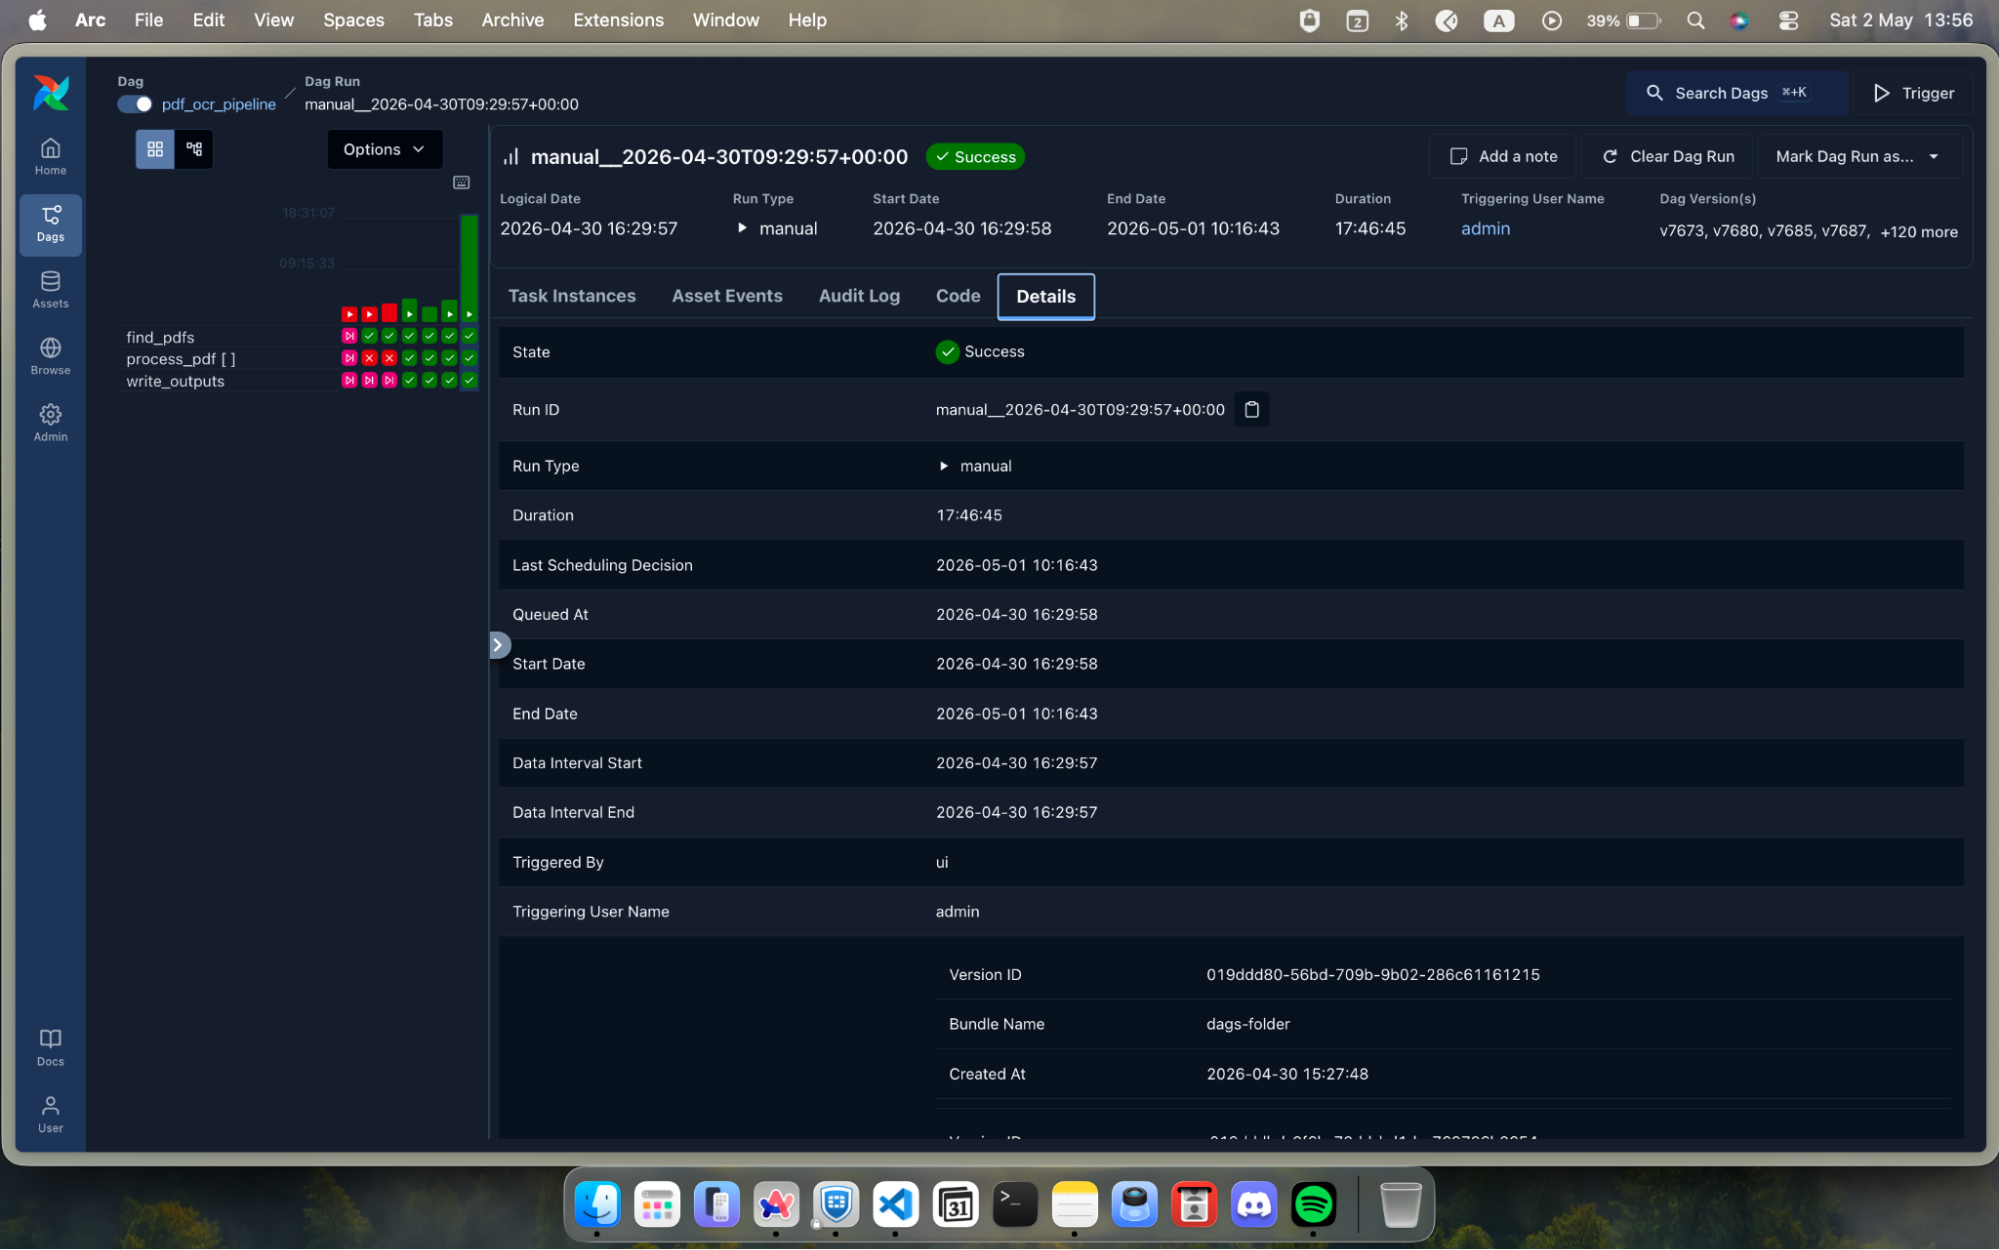
\includegraphics[width=0.95\textwidth]{figures/image16.png}
\caption{Apache Airflow \texttt{pdf\_ocr\_pipeline} DAG run detail}\label{fig:pdf-run}
\end{figure}

At the current stage, the \texttt{pdf\_ocr\_pipeline} DAG is stable and runs reliably on its daily schedule. New PDF files uploaded to the MinIO \texttt{raw/} prefix are correctly discovered, processed through the hybrid PyMuPDF + Typhoon-OCR pipeline, and produce both clean training-text outputs in the result JSONL and rich diagnostic information in the meta JSONL.

\newpage
\subsection{Unstructured Audio ASR Pipeline}

The audio ASR pipeline is orchestrated using Apache Airflow in a DAG named \texttt{audio\_asr\_pipeline}. This DAG runs on a daily schedule and is designed to detect new audio files in MinIO, transcribe them with a Thai/Isan Whisper-based ASR service, and write both the clean transcripts and detailed quality metadata back to MinIO. The DAG supports two input formats: standalone audio files (\texttt{.wav}, \texttt{.mp3}, \texttt{.flac}, \texttt{.m4a}, \texttt{.ogg}, \texttt{.opus} and other common containers) and Parquet datasets in which each row carries an embedded audio payload together with an optional ground-truth transcription.

\begin{figure}[H]\centering
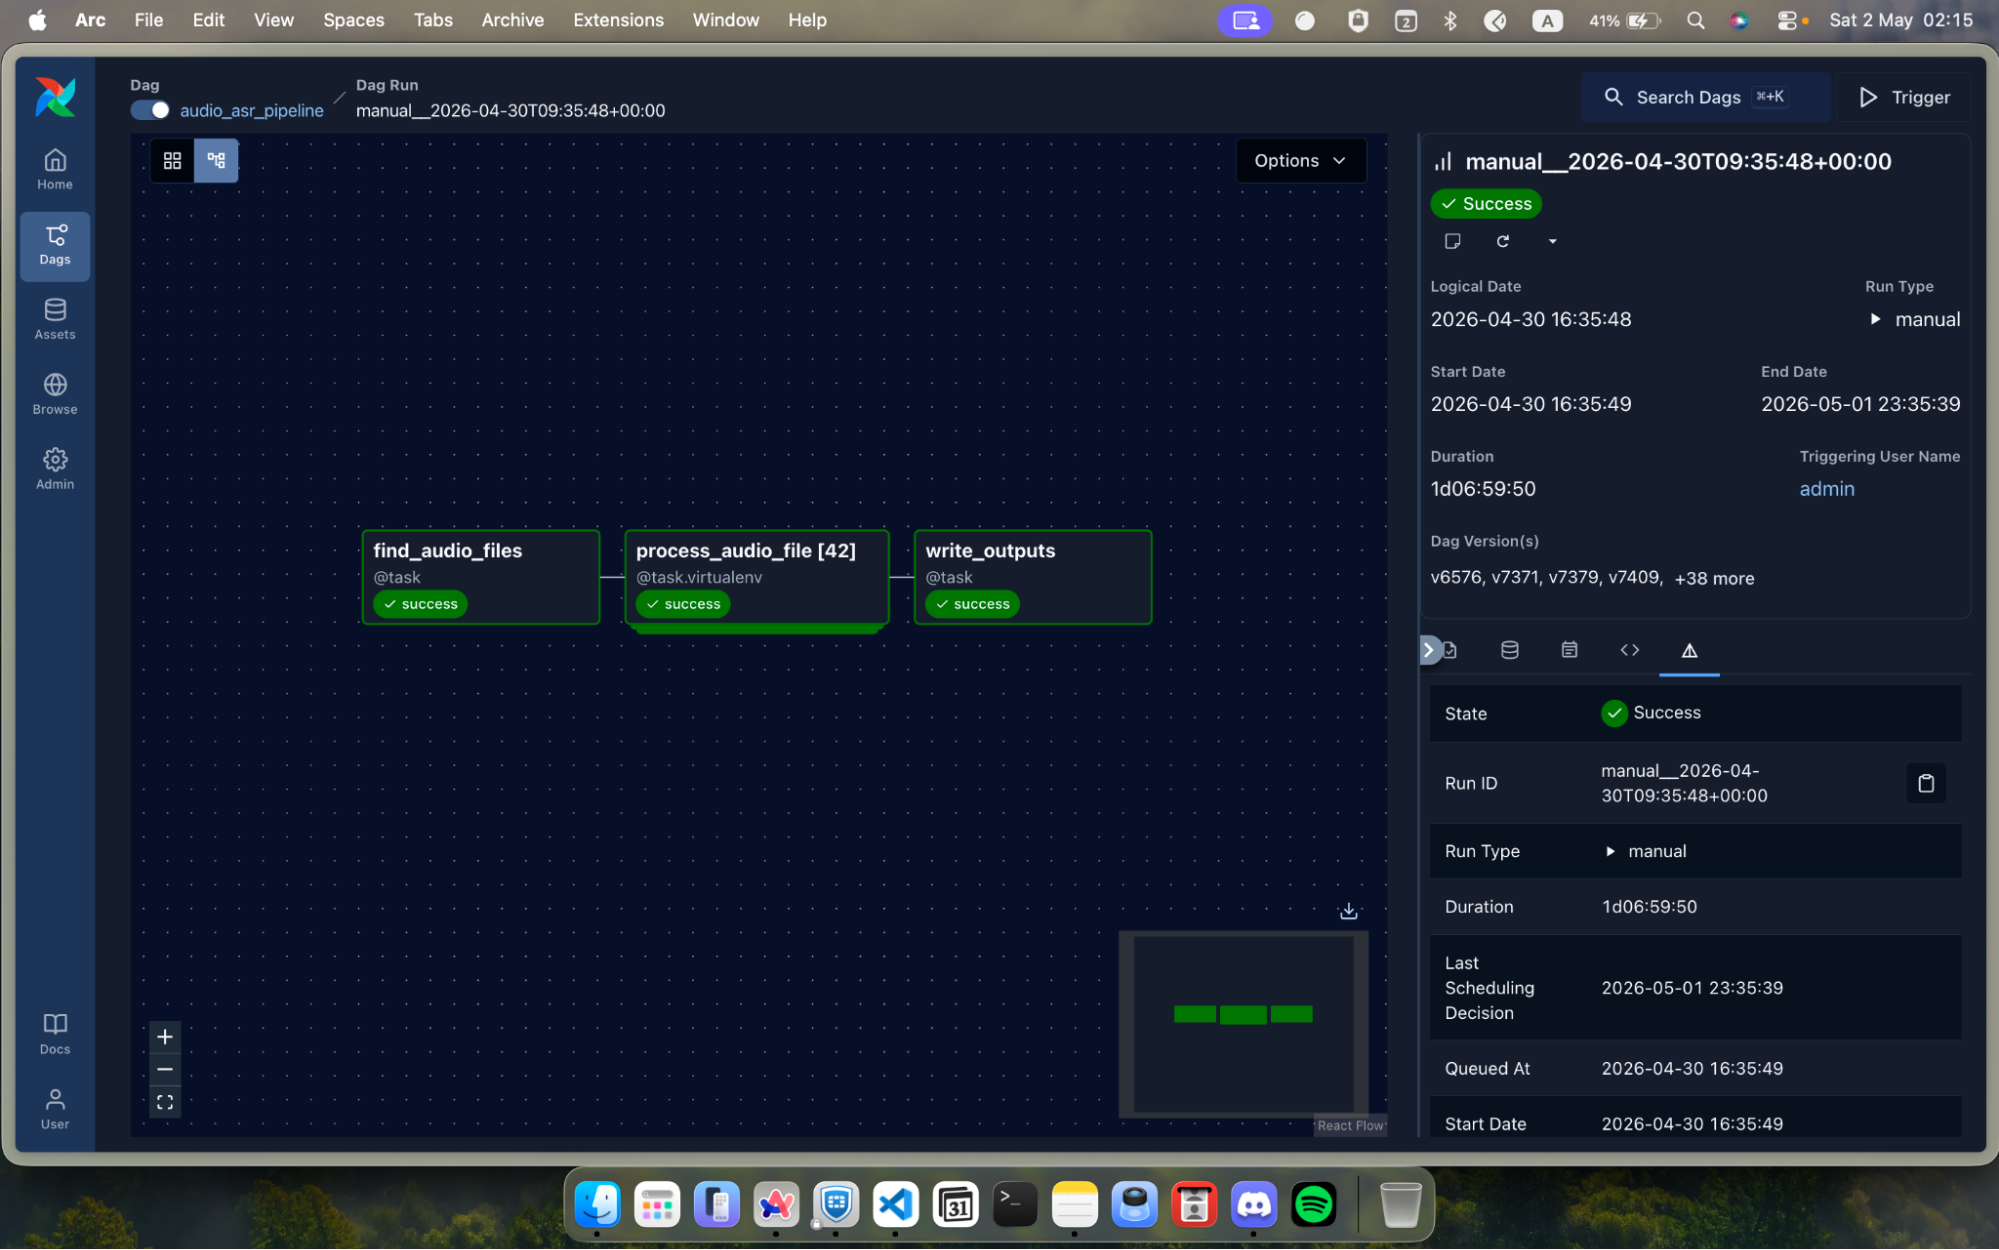
\includegraphics[width=0.95\textwidth]{figures/image27.png}
\caption{Apache Airflow graph view of \texttt{audio\_asr\_pipeline}}\label{fig:audio-graph}
\end{figure}

The first task, \texttt{find\_audio\_files}, lists every object under the configured \texttt{raw/} prefix across all buckets and selects files whose extensions match either the supported audio formats or \texttt{.parquet}. Once the list is built, the DAG uses dynamic task mapping to fan out into one \texttt{process\_audio\_file} instance per discovered file. Mapped tasks are bound to the dedicated \texttt{asr\_pool} Airflow pool with up to eight concurrent instances per DAG run, and each task in turn spawns its own internal pool of eight worker threads, giving an effective fan-out of roughly thirty-two concurrent ASR requests against the GPU server.

\begin{figure}[H]\centering
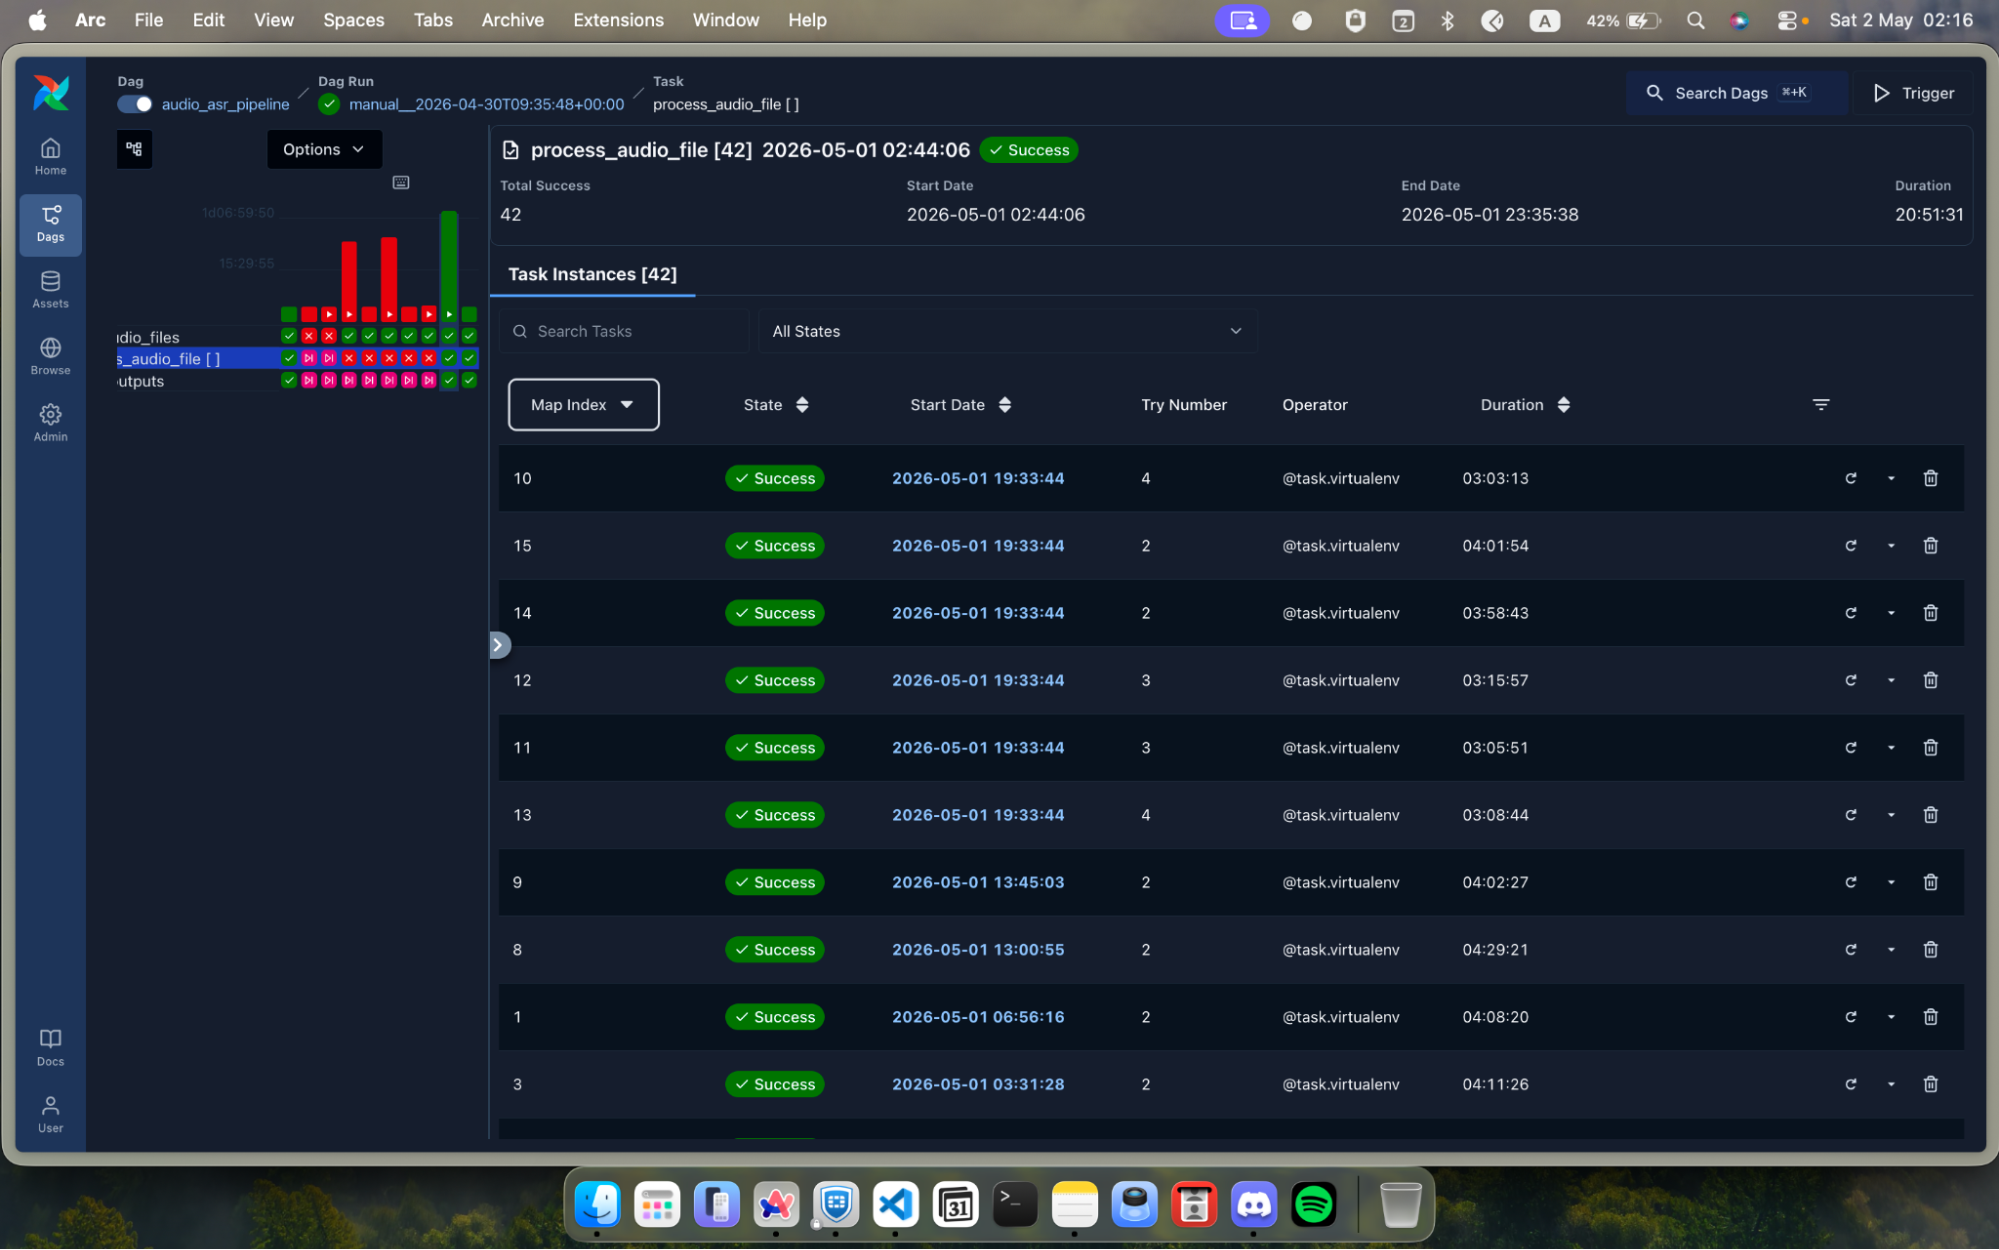
\includegraphics[width=0.9\textwidth]{figures/image18.png}
\caption{Apache Airflow \texttt{process\_audio\_file} task detail}\label{fig:audio-process}
\end{figure}

Inside each \texttt{process\_audio\_file} task, the pipeline first checks the health of the ASR endpoint and reads any previously generated result and meta JSONL files so that already-transcribed rows can be skipped. The processing logic then branches on the file type. For standalone audio files, the task downloads the bytes from MinIO, measures the duration and either transcribes the file in a single request or, if the audio exceeds the configured split threshold of 300 seconds, decodes it to 16~kHz mono with PyAV and splits it into approximately 30-second WAV segments that are transcribed independently and then merged into a single record. For Parquet inputs, the task iterates over the file in batches using \texttt{pyarrow}, extracts the audio bytes and any ground-truth column from each row, and dispatches the rows to a \texttt{ThreadPoolExecutor}.

Each transcription is then evaluated by a quality function. When ground truth is available (Path A), the function computes the Character Error Rate between the hypothesis and the reference after applying Thai-specific normalization. If the initial CER exceeds the configured threshold, the function attempts a series of recovery strategies: stripping trailing Whisper repetition loops, expanding known abbreviations on the ground-truth side, retrying decoding at a higher temperature and applying a foreign-word recovery rule. When ground truth is missing (Path B), the function instead checks that the output is non-trivial, free of repetition loops and consistent with a secondary higher-temperature transcription on sufficiently long clips. Successful rows are written to the result JSONL, while low-quality, silent or failed rows are written to the meta JSONL together with a quality reason, the measured duration, the CER and abbreviation hints when applicable.

\begin{figure}[H]\centering
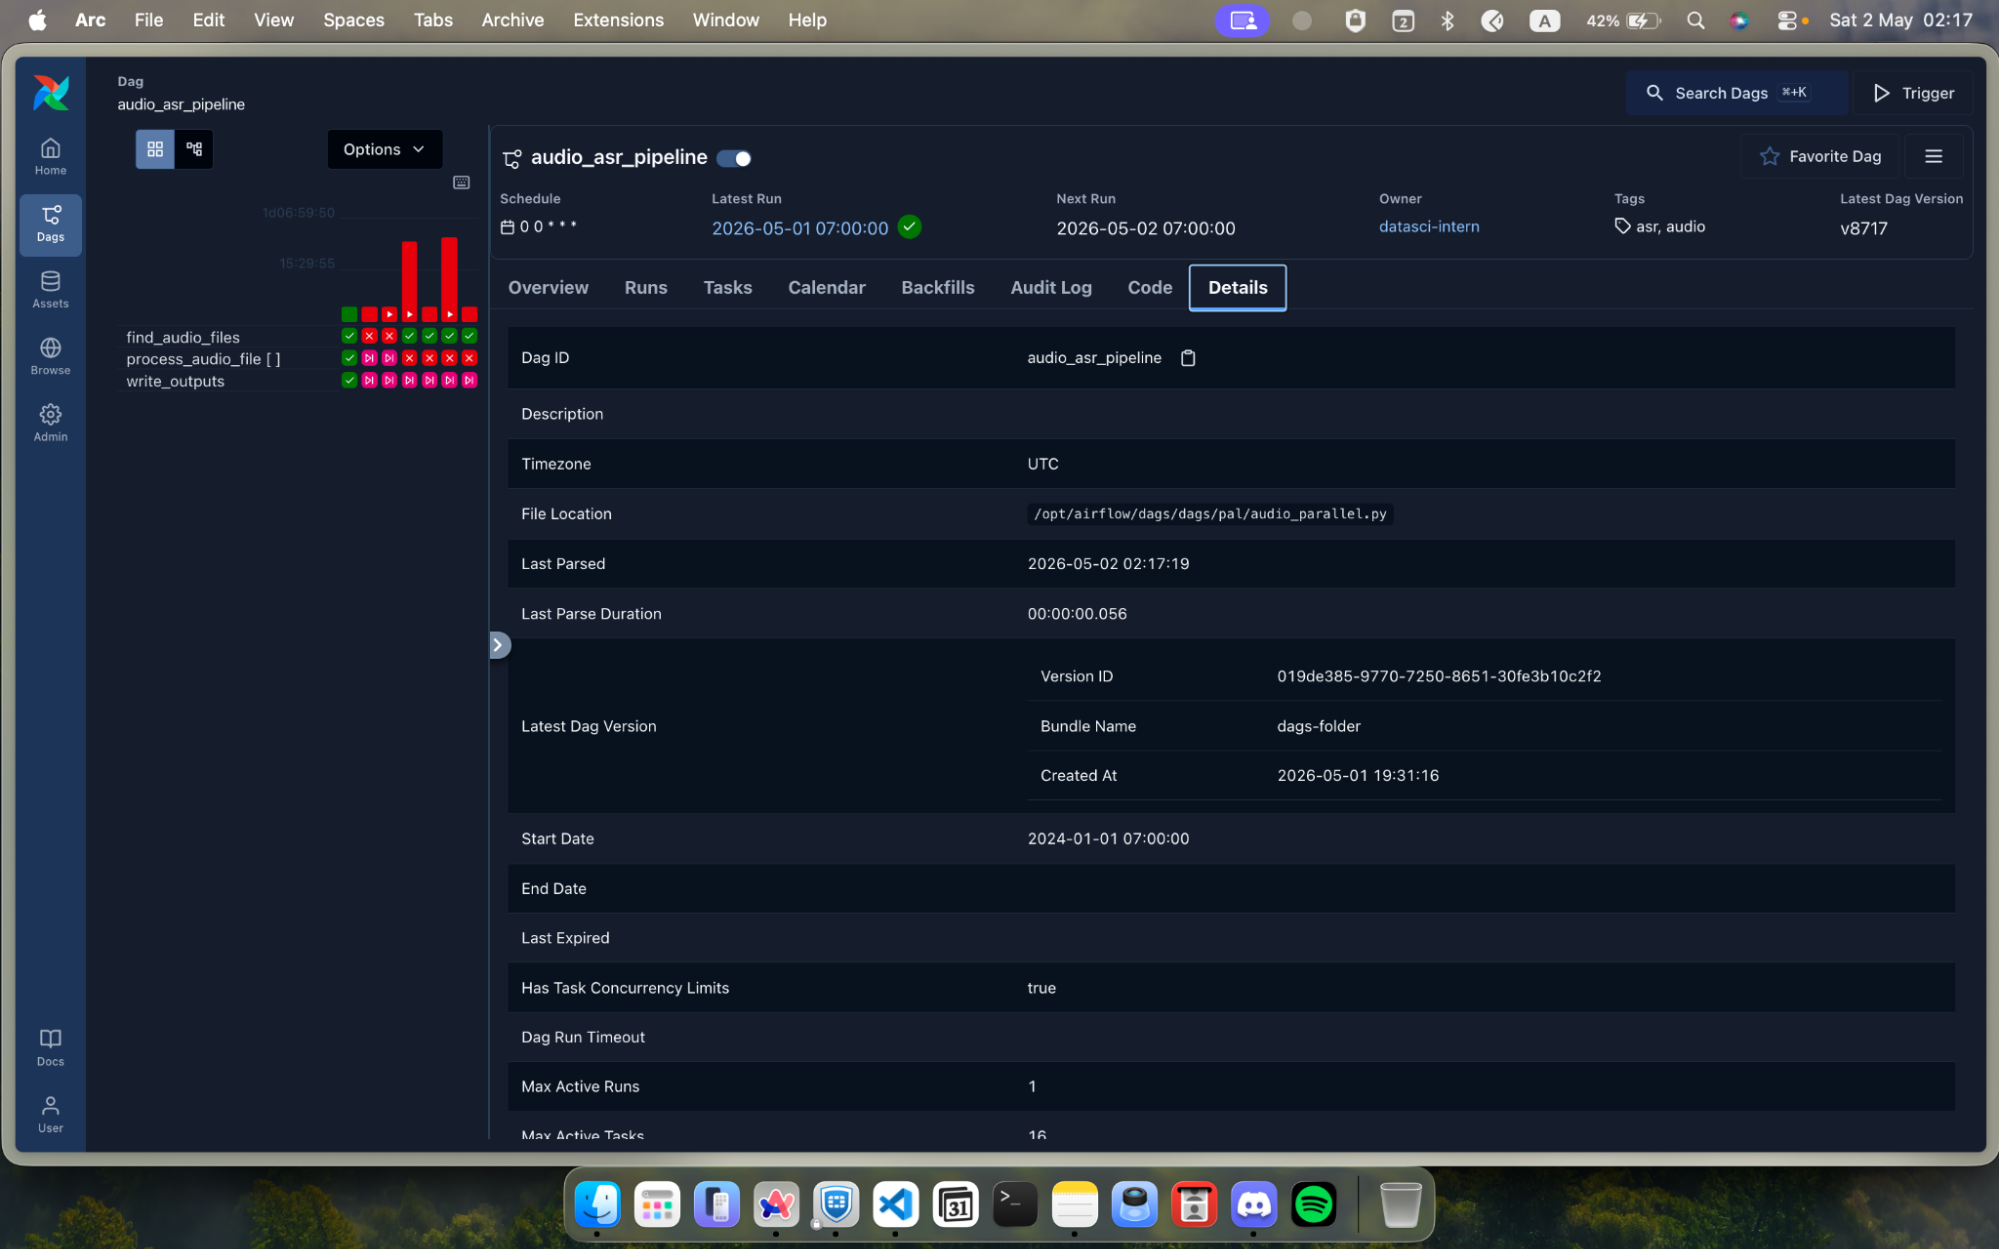
\includegraphics[width=0.95\textwidth]{figures/image15.png}
\caption{Apache Airflow \texttt{audio\_asr\_pipeline} DAG run detail}\label{fig:audio-run}
\end{figure}

After all chunks have been processed, the task performs a final deduplication pass over both output JSONL files using last-write-wins semantics keyed on filename, records per-file quality statistics and returns this summary to the DAG. The downstream \texttt{write\_outputs} task aggregates these per-file summaries into a global report.
\newpage
\section{Monitoring}

For this project, a monitoring system was implemented using Prometheus and Grafana to track the health and performance of the whole data pipeline. All monitoring services run as Docker containers in the same environment as Airflow, MinIO and PostgreSQL.

\subsection{Metrics Collection with Prometheus}

Prometheus is used as the metrics collector. It is configured through a \texttt{prometheus.yml} file, where each component is defined as a separate scrape job with its endpoint and port. Prometheus regularly calls the metrics endpoint of each exporter and stores the results in its time-series database.

\begin{figure}[H]\centering
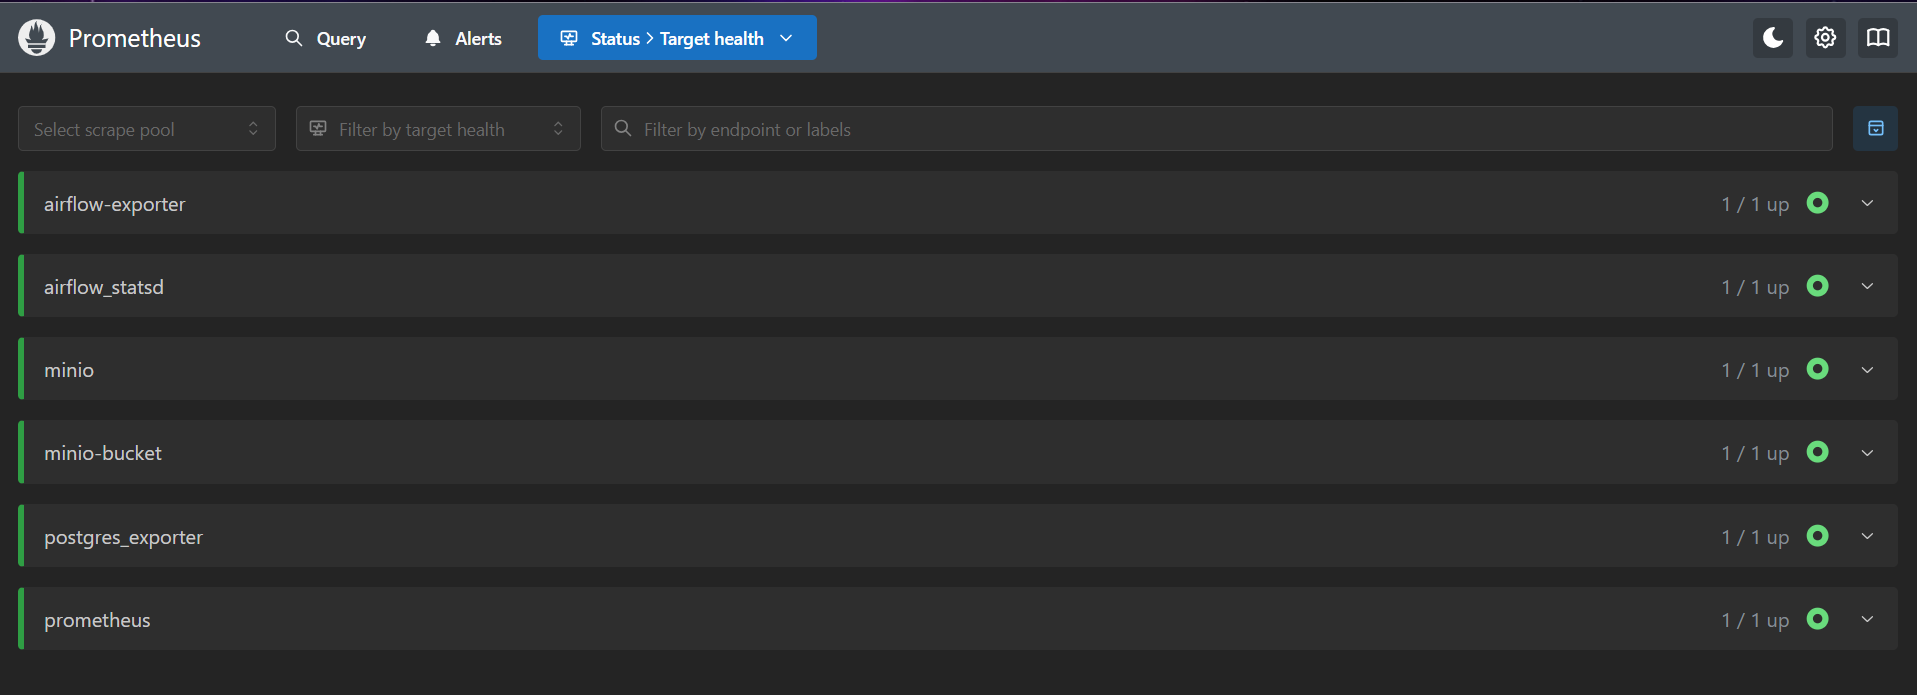
\includegraphics[width=0.9\textwidth]{figures/image25.png}
\caption{Prometheus metric connector}\label{fig:prom-targets}
\end{figure}

\begin{itemize}
\item \textbf{Airflow exporter and \texttt{airflow\_statsd}} export DAG and task metrics from the Airflow webserver and scheduler. These metrics include DAG run status, task duration, number of retries and scheduler activity.
\item \textbf{MinIO and \texttt{minio-bucket}} exporters expose metrics from the object storage. One focuses on cluster status (disk usage, read/write operations, latency), while the bucket exporter reports bucket-level information.
\item \textbf{Postgres exporter} reads internal statistics from PostgreSQL and exposes metrics like query duration, number of connections, table size and cache hit rate.
\item \textbf{Prometheus} itself is also scraped, allowing basic self-monitoring.
\end{itemize}

In the Prometheus ``Targets'' page, all these jobs appear as separate targets, and the status ``1/1 up'' confirms that Prometheus can successfully connect to each exporter and collect metrics on a regular schedule.
\newpage
\subsection{Grafana Dashboard}

Grafana is connected to Prometheus as a single data source by pointing it to the Prometheus HTTP endpoint. All dashboards use PromQL queries to read metrics from Prometheus and display them as graphs, tables and single-value panels. To keep things organized, the dashboards are grouped into folders by component.

\begin{figure}[H]\centering
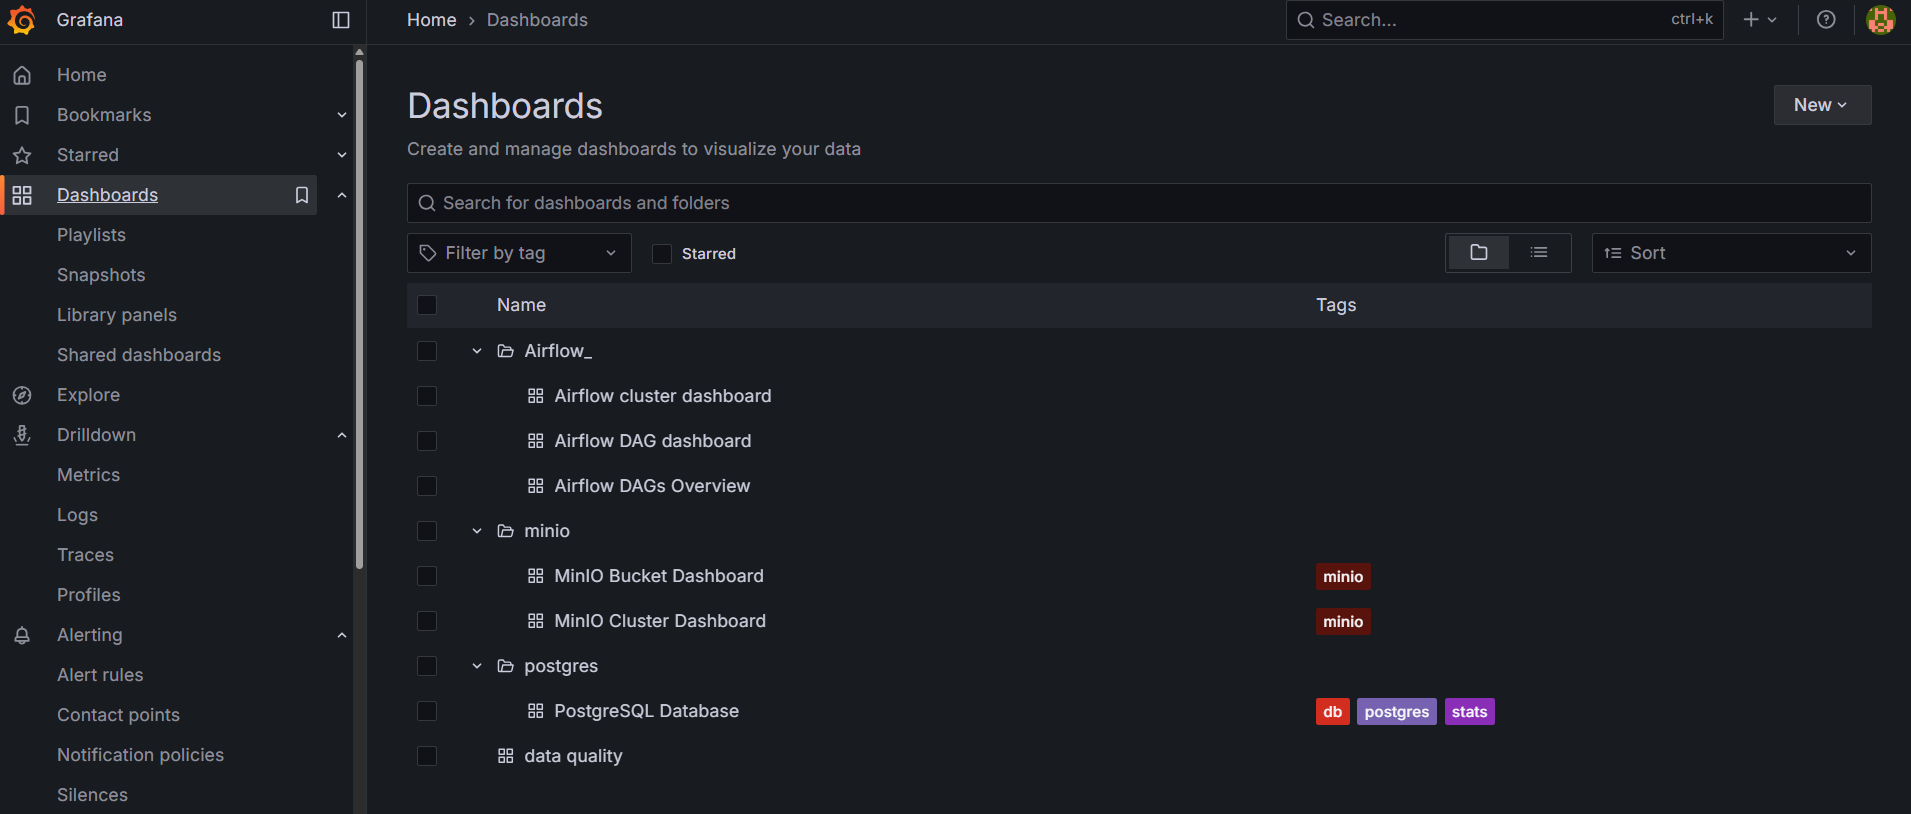
\includegraphics[width=0.95\textwidth]{figures/image13.png}
\caption{Grafana Dashboard}\label{fig:grafana}
\end{figure}

Overall, this monitoring setup gives a single place to see whether the pipeline is running, how long it takes, how much data is stored and whether the data-quality checks behave as expected. This information is later used as the basis for alert rules so that problems in Airflow, MinIO or PostgreSQL can be detected early.

%%%%%%%%%%%%%%%%%%%%%%%%%%%%%%%%%%%%%%%%%%%%%%%%%%%%%%%%%%%%%%
%%%%%%%%%%%%%%%  CHAPTER 4  %%%%%%%%%%%%%%%%%%%%%%%%%%%%%%%%%%
%%%%%%%%%%%%%%%%%%%%%%%%%%%%%%%%%%%%%%%%%%%%%%%%%%%%%%%%%%%%%%
\chapter{Results and Discussion}

\section{Data Lake}

The MinIO bucket \texttt{ai-datasets} is organized into multiple layers to support different stages of the data processing pipeline. Within the \texttt{raw/} directory, datasets are further organized by source. This structure ensures that data from multiple domains and sources can be managed efficiently and allows easy extension when new datasets are added to the system. The organization aligns with the dataset catalog used in the project, which includes multiple domains such as finance, medical, tourism and legal.

\begin{figure}[H]\centering
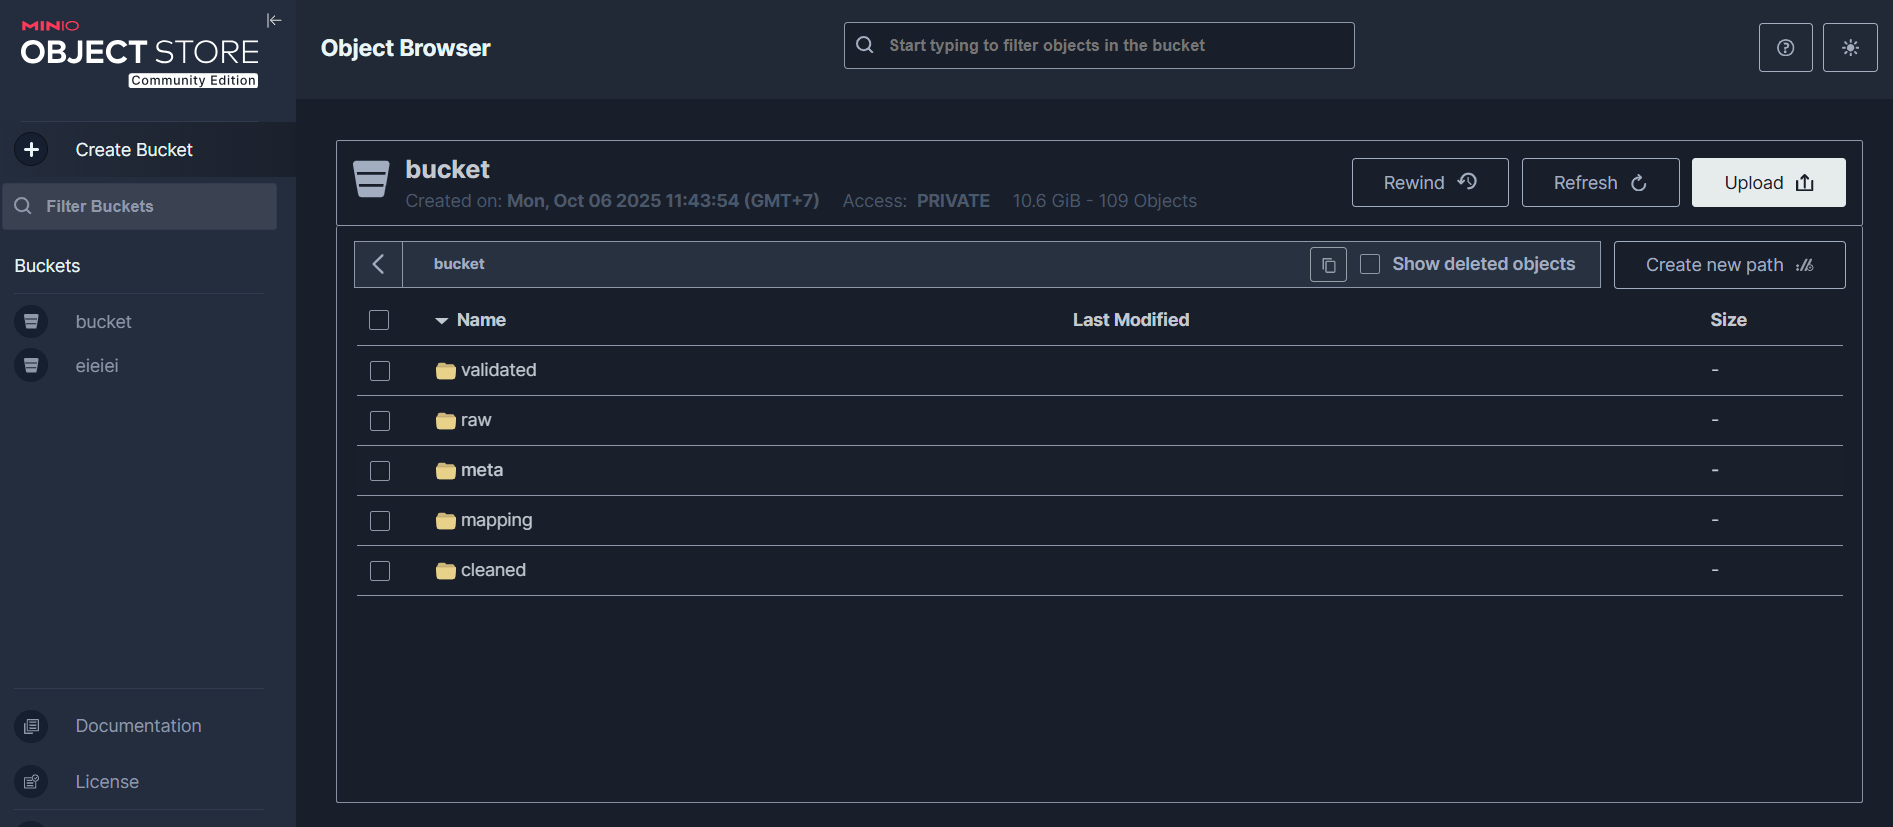
\includegraphics[width=0.9\textwidth]{figures/image30.png}
\caption{Datalake Layer}\label{fig:datalake-layer}
\end{figure}

\begin{figure}[H]\centering
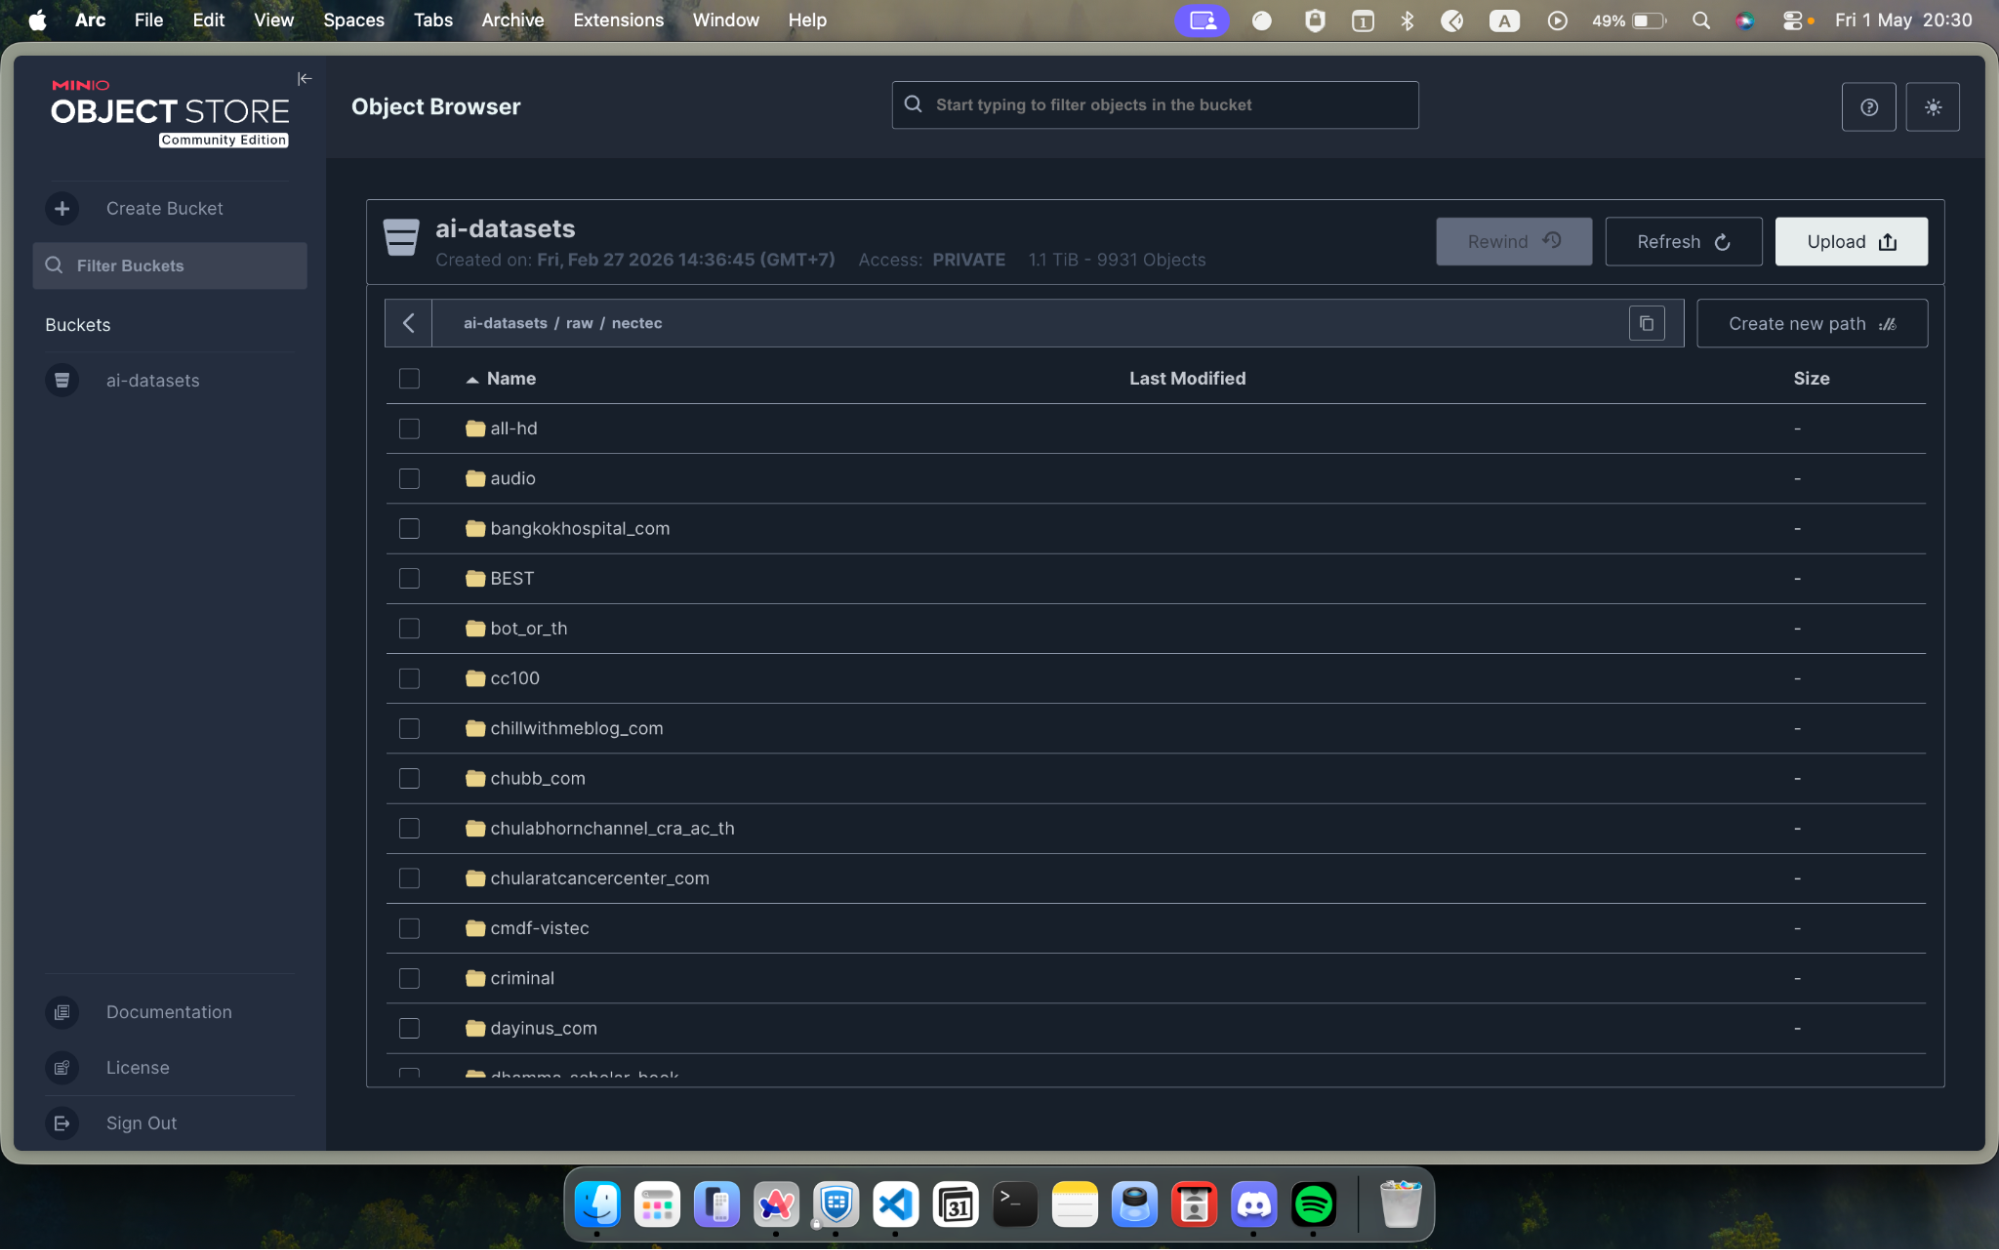
\includegraphics[width=0.9\textwidth]{figures/image9.png}
\caption{NECTEC Datasets in MinIO}\label{fig:nectec-minio}
\end{figure}

\section{Unstructured Pipeline}

The unstructured pipeline was developed to process data that does not already exist in a structured table format. In this project, the unstructured pipeline consists of two main components: the PDF pipeline and the audio pipeline. The PDF pipeline extracts Thai text from both text-native and image-heavy PDF files, while the audio pipeline converts Thai speech into text using an Automatic Speech Recognition (ASR) model.

\begin{table}[H]
\centering
\caption{Overall unstructured pipeline output}\label{tbl:unstructured-overview}
\begin{tabular}{|p{0.25\textwidth}|p{0.30\textwidth}|p{0.30\textwidth}|}
\hline
\textbf{Pipeline} & \textbf{Records / Documents} & \textbf{Output volume} \\ \hline
PDF pipeline & 133 documents / 7{,}346 pages & 8.42 million characters \\ \hline
Audio pipeline & 307{,}793 utterances & 19.42 million characters / 656.93 audio hours \\ \hline
Total & --- & 27.85 million characters \\ \hline
\end{tabular}
\end{table}

In conclusion, the unstructured pipeline successfully converted both PDF and audio data into AI-ready text outputs. The PDF pipeline extracted 8.42 million characters from Thai PDF documents, while the audio pipeline generated 19.42 million characters from Thai speech data. Together, both pipelines produced approximately 27.85 million characters of usable text data.

\subsection{PDF Pipeline}

The PDF pipeline was evaluated using a Thai-language PDF corpus from NECTEC. The dataset was divided into two sub-corpora: \texttt{pdf1} and \texttt{pdf2}. The \texttt{pdf1} dataset mainly contains text-native PDFs, while \texttt{pdf2} mainly contains image-heavy or scanned PDF documents. In total, the pipeline processed 133 PDF documents containing 7{,}346 pages and 1{,}211.6~MB of data.

\begin{table}[H]
\centering
\caption{PDF dataset overview}\label{tbl:pdf-overview}
\begin{tabular}{|p{0.18\textwidth}|p{0.22\textwidth}|c|c|c|}
\hline
\textbf{Dataset} & \textbf{Document type} & \textbf{Documents} & \textbf{Pages} & \textbf{Size (MB)} \\ \hline
pdf1 & Text-native PDFs & 94 & 5{,}181 & 693.6 \\ \hline
pdf2 & Image-heavy PDFs & 39 & 2{,}165 & 518.1 \\ \hline
Total & Mixed PDF corpus & 133 & 7{,}346 & 1{,}211.6 \\ \hline
\end{tabular}
\end{table}

At the document level, the pipeline successfully processed all PDF files. Both \texttt{pdf1} and \texttt{pdf2} achieved a 100\% document success rate, with no failed documents.

\begin{table}[H]
\centering
\caption{PDF document-level results}\label{tbl:pdf-doc}
\begin{tabular}{|p{0.32\textwidth}|c|c|c|}
\hline
\textbf{Metric} & \textbf{pdf1} & \textbf{pdf2} & \textbf{Combined} \\ \hline
Documents processed & 94 & 39 & 133 \\ \hline
Documents succeeded & 94 (100\%) & 39 (100\%) & 133 (100\%) \\ \hline
Documents failed & 0 & 0 & 0 \\ \hline
Total pages & 5{,}181 & 2{,}165 & 7{,}346 \\ \hline
Average pages / document & 55.1 & 55.5 & 55.2 \\ \hline
Total characters extracted & 5{,}823{,}040 & 2{,}601{,}378 & 8{,}424{,}418 \\ \hline
Total processing time & 174.5 min & 152.9 min & 327.4 min \\ \hline
Average time / document & 111.4 sec & 235.2 sec & --- \\ \hline
\end{tabular}
\end{table}

Although \texttt{pdf2} contained fewer documents than \texttt{pdf1}, it required more time per document because most pages were image-heavy and needed OCR processing. This shows that scanned or image-based PDFs require more computational resources than text-native PDFs.

\begin{table}[H]
\centering
\caption{PDF page-level results}\label{tbl:pdf-page}
\begin{tabular}{|p{0.20\textwidth}|c|c|c|}
\hline
\textbf{Page status} & \textbf{pdf1} & \textbf{pdf2} & \textbf{Combined} \\ \hline
Success & 4{,}960 (95.7\%) & 2{,}032 (93.9\%) & 6{,}992 (95.2\%) \\ \hline
Low quality & 11 (0.2\%) & 11 (0.5\%) & 22 (0.3\%) \\ \hline
Empty & 210 (4.1\%) & 122 (5.6\%) & 332 (4.5\%) \\ \hline
Failed & 0 & 0 & 0 \\ \hline
\end{tabular}
\end{table}

The PDF pipeline used a hybrid extraction method. It used PyMuPDF as the primary text extractor and applied OCR only when direct text extraction was not sufficient. This approach improved efficiency because text-native pages could be processed quickly without OCR, while image-heavy pages could still be recovered through OCR.

\begin{table}[H]
\centering
\caption{PDF extraction method results}\label{tbl:pdf-method}
\begin{tabular}{|p{0.32\textwidth}|p{0.28\textwidth}|p{0.28\textwidth}|}
\hline
\textbf{Metric} & \textbf{pdf1} & \textbf{pdf2} \\ \hline
Pages routed to PyMuPDF & 3{,}730 (72.0\%) & 580 (26.8\%) \\ \hline
Pages routed to OCR & 1{,}451 (28.0\%) & 1{,}585 (73.2\%) \\ \hline
OCR page-success rate & 1{,}230 / 1{,}451 (84.8\%) & 1{,}452 / 1{,}585 (91.6\%) \\ \hline
Character share from PyMuPDF & 5{,}312{,}126 (92.9\%) & 617{,}743 (24.6\%) \\ \hline
Character share from OCR & 408{,}645 (7.1\%) & 1{,}892{,}446 (75.4\%) \\ \hline
Documents needing OCR only & 0 & 22 (56.4\%) \\ \hline
Documents using both methods & 94 (100\%) & 17 (43.6\%) \\ \hline
\end{tabular}
\end{table}

The results show that the hybrid method was important for both datasets. In \texttt{pdf1}, most text was extracted using PyMuPDF because the documents were mainly text-native. In \texttt{pdf2}, most text came from OCR because the documents were image-heavy. The PDF pipeline achieved reliable results for both text-native and image-heavy PDF files. Key findings:
\begin{itemize}
\item The pipeline achieved 100\% document-level success.
\item The combined page success rate was 95.2\% with no failed pages.
\item The hybrid extraction strategy was effective.
\item The \texttt{pdf2} dataset required more OCR processing because it contained more scanned and image-heavy layouts.
\item The low-quality rate was only 0.3\%, showing that the quality gate successfully removed unreliable outputs.
\item Empty pages were excluded intentionally to reduce the risk of hallucinated text entering the final training dataset.
\end{itemize}
\newpage
\subsection{Audio Pipeline}

The audio pipeline was evaluated using a NECTEC Thai-central audio corpus. The dataset was stored as 16 Parquet shards, each containing audio bytes with corresponding ground-truth Thai transcripts. The pipeline used the Typhoon Isan ASR Whisper model to convert speech into text. In total, the pipeline processed 335{,}674 audio rows.

\begin{table}[H]
\centering
\caption{Audio dataset overview}\label{tbl:audio-overview}
\begin{tabular}{|p{0.30\textwidth}|p{0.55\textwidth}|}
\hline
\textbf{Metric} & \textbf{Value} \\ \hline
Dataset source & NECTEC Thai-central audio corpus \\ \hline
Number of shards & 16 Parquet shards \\ \hline
Total rows processed & 335{,}674 \\ \hline
Model used & typhoon-ai/typhoon-isan-asr-whisper \\ \hline
Main quality metric & Character Error Rate (CER) \\ \hline
Acceptance threshold & CER $\leq$ 0.20 \\ \hline
\end{tabular}
\end{table}

\begin{table}[H]
\centering
\caption{Audio acceptance results}\label{tbl:audio-accept}
\begin{tabular}{|p{0.40\textwidth}|c|c|}
\hline
\textbf{Outcome} & \textbf{Count} & \textbf{Percentage} \\ \hline
Kept / Success & 307{,}793 & 91.69\% \\ \hline
Filtered as low quality & 27{,}260 & 8.12\% \\ \hline
Filtered as silent audio & 621 & 0.19\% \\ \hline
Failed / server empty & 0 & 0.00\% \\ \hline
Total & 335{,}674 & 100.00\% \\ \hline
\end{tabular}
\end{table}

The pipeline kept 307{,}793 records, representing 91.69\% of all input rows. This high acceptance rate shows that most audio samples were successfully transcribed with acceptable quality. The pipeline also produced zero failed or server-empty records, indicating that the ASR workflow was stable.

\begin{table}[H]
\centering
\caption{Audio output volume}\label{tbl:audio-volume}
\begin{tabular}{|p{0.40\textwidth}|p{0.40\textwidth}|}
\hline
\textbf{Metric} & \textbf{Value} \\ \hline
Kept transcripts & 307{,}793 records \\ \hline
Total audio kept & 656.93 hours \\ \hline
Total audio kept & 2{,}364{,}958 seconds \\ \hline
Total transcript characters & 19{,}423{,}129 \\ \hline
Average characters / utterance & 63.1 \\ \hline
\end{tabular}
\end{table}

The accepted records showed strong transcription quality. The mean CER was 0.0447 and the median CER was 0.0270. In addition, 38.2\% of accepted utterances had a perfect CER of 0, meaning the predicted transcription exactly matched the ground-truth transcript.

\begin{table}[H]
\centering
\caption{CER distribution of accepted records}\label{tbl:cer-accept}
\begin{tabular}{|p{0.40\textwidth}|p{0.30\textwidth}|}
\hline
\textbf{Statistic} & \textbf{Value} \\ \hline
Mean CER & 0.0447 \\ \hline
Median CER & 0.0270 \\ \hline
25th percentile & 0.0000 \\ \hline
75th percentile & 0.0741 \\ \hline
90th percentile & 0.1250 \\ \hline
Records with CER = 0 & 117{,}619 (38.2\%) \\ \hline
Records with CER $<$ 0.05 & 196{,}716 (63.9\%) \\ \hline
Records with CER $<$ 0.10 & 256{,}590 (83.4\%) \\ \hline
\end{tabular}
\end{table}

\begin{table}[H]
\centering
\caption{CER distribution of filtered records}\label{tbl:cer-filtered}
\begin{tabular}{|p{0.40\textwidth}|p{0.30\textwidth}|}
\hline
\textbf{Statistic} & \textbf{Value} \\ \hline
Mean CER & 0.3618 \\ \hline
Median CER & 0.2909 \\ \hline
Minimum CER & 0.2007 \\ \hline
Maximum CER & 11.0857 \\ \hline
Quality reason & high\_cer \\ \hline
\end{tabular}
\end{table}

The rejected records likely included incorrect transcriptions, noisy audio, wrong-language outputs or other ASR errors. Most accepted audio clips were short utterances. The median duration was 6.40 seconds, while the mean duration was 7.68 seconds.

\begin{table}[H]
\centering
\caption{Audio duration profile of accepted records}\label{tbl:audio-duration}
\begin{tabular}{|p{0.40\textwidth}|p{0.30\textwidth}|}
\hline
\textbf{Metric} & \textbf{Duration} \\ \hline
Mean duration & 7.68 sec \\ \hline
Median duration & 6.40 sec \\ \hline
90th percentile & 14.51 sec \\ \hline
99th percentile & 21.16 sec \\ \hline
Maximum duration & 61.18 sec \\ \hline
\end{tabular}
\end{table}

\begin{table}[H]
\centering
\caption{Per-shard result consistency}\label{tbl:per-shard}
\begin{tabular}{|p{0.40\textwidth}|p{0.40\textwidth}|}
\hline
\textbf{Metric} & \textbf{Range across 16 shards} \\ \hline
Kept rows & 19{,}138 -- 19{,}278 \\ \hline
Average CER of accepted records & 0.0441 -- 0.0451 \\ \hline
Audio hours kept & 40.66 -- 41.30 \\ \hline
Filtered low-quality records & 1{,}661 -- 1{,}803 \\ \hline
Silent audio records & 28 -- 48 \\ \hline
\end{tabular}
\end{table}

The variation across shards was less than 1\% for the main metrics. To verify that the audio pipeline was not limited to a specific audio container or codec, an audio format compatibility test was conducted. The same Thai news audio clip, named \texttt{sukie-test}, was encoded into 13 different audio formats and processed through the full ASR pipeline.

\begin{table}[H]
\centering
\caption{Audio format compatibility test results}\label{tbl:audio-format}
\small
\begin{tabular}{|c|c|p{0.32\textwidth}|c|c|}
\hline
\textbf{No.} & \textbf{Format} & \textbf{Container / Codec family} & \textbf{Status} & \textbf{Transcript chars} \\ \hline
1 & .wav & PCM, uncompressed & Success & 259 \\ \hline
2 & .flac & Free Lossless Audio Codec & Success & 259 \\ \hline
3 & .aiff & Apple uncompressed & Success & 259 \\ \hline
4 & .au & Sun/NeXT $\mu$-law & Success & 259 \\ \hline
5 & .mp3 & MPEG-1/2 Layer III & Success & 259 \\ \hline
6 & .aac & Advanced Audio Coding & Success & 258 \\ \hline
7 & .m4a & MP4 container / AAC audio & Success & 259 \\ \hline
8 & .mp4 & MP4 container, audio track & Success & 259 \\ \hline
9 & .ogg & Ogg Vorbis & Success & 259 \\ \hline
10 & .opus & Opus & Success & 259 \\ \hline
11 & .webm & WebM container / Opus & Success & 259 \\ \hline
12 & .wma & Windows Media Audio & Success & 258 \\ \hline
13 & .3gp & 3GPP, mobile & Success & 259 \\ \hline
\end{tabular}
\end{table}

The result shows that 13 out of 13 formats were successfully decoded and transcribed, giving a 100\% format success rate. This is important because audio data collected from different sources may not always follow a single standard format. To verify that the result was not dependent on only one source clip, the same test was repeated using a different short 6.4-second Thai utterance: \textthai{``ทีมจากอิสราเอลไม่ควรได้เป็นเจ้าบ้านในเกมยูฟ่าครับ''}.

\begin{table}[H]
\centering
\caption{Format compatibility replication results}\label{tbl:audio-format-rep}
\small
\begin{tabular}{|p{0.22\textwidth}|p{0.18\textwidth}|c|c|p{0.22\textwidth}|}
\hline
\textbf{Format group} & \textbf{Formats} & \textbf{Status} & \textbf{Chars} & \textbf{Transcript result} \\ \hline
Lossless / uncompressed & .wav, .flac, .aiff, .au & Success & 49 & Identical Thai sentence \\ \hline
MP / AAC family & .mp3, .aac, .m4a, .mp4 & Success & 49 & Identical Thai sentence \\ \hline
Open web formats & .ogg, .opus, .webm & Success & 49 & Identical Thai sentence \\ \hline
Legacy / mobile formats & .wma, .3gp & Success & 49 & Identical Thai sentence \\ \hline
\end{tabular}
\end{table}

\begin{table}[H]
\centering
\caption{Combined format-coverage summary}\label{tbl:audio-format-combined}
\small
\begin{tabular}{|p{0.18\textwidth}|p{0.18\textwidth}|c|c|c|p{0.22\textwidth}|}
\hline
\textbf{Test set} & \textbf{Source clip} & \textbf{Duration (s)} & \textbf{Formats} & \textbf{Successful} & \textbf{Byte stability} \\ \hline
test\_audio\_formats & Thai news clip & $\sim$30 & 13 & 13/13 (100\%) & 11/13 (84.6\%) \\ \hline
test\_audio & Thai single sentence & 6.4 & 13 & 13/13 (100\%) & 13/13 (100\%) \\ \hline
Combined & --- & --- & 26 trials & 26/26 (100\%) & 24/26 (92.3\%) \\ \hline
\end{tabular}
\end{table}

The audio pipeline achieved strong results in transforming Thai speech data into AI-ready text transcripts. Key findings:
\begin{itemize}
\item The pipeline accepted 91.69\% of all audio records after applying the CER quality gate.
\item The final accepted set contained 656.93 hours of audio and 19.42 million transcript characters.
\item The mean CER of accepted records was only 0.0447.
\item 38.2\% of accepted records had a perfect CER of 0.
\item The pipeline filtered out 8.12\% low-quality records.
\item Silent-audio detection removed 0.19\% of records that did not contain meaningful speech.
\item No failed or server-empty records appeared in the final output.
\item The format compatibility tests showed 100\% success across 26 format-clip trials.
\end{itemize}

One important reason for using CER instead of WER is that Thai language does not always separate words with spaces. CER is more suitable for this project because it evaluates transcription quality at the character level.
\newpage
\section{JSONL Pipeline}

\subsection{Main Pipeline Execution}

The main pipeline demonstrates a successful execution of the end-to-end workflow. The DAG consists of multiple tasks that handle different stages of the data ingestion and preparation process. Key steps in the pipeline include:
\begin{itemize}
\item \texttt{wait\_raw\_stable}: waits for new data to be available in the storage system
\item \texttt{list\_raw\_keys}: retrieves file paths from the data lake (MinIO)
\item \texttt{choose\_keys}: selects relevant datasets for processing
\item \texttt{filter\_new}: filters out already processed or duplicate data
\item \texttt{build\_envs}: prepares runtime environment and parameters
\item \texttt{run\_pipeline\_all}: executes the main processing logic
\item \texttt{to\_label\_params} / \texttt{to\_log\_params}: prepares parameters for labeling and logging
\item \texttt{sentiment\_upsert\_mapped}: stores processed results into the database
\item \texttt{log\_ingest}: logs ingestion results
\end{itemize}

\begin{figure}[H]\centering
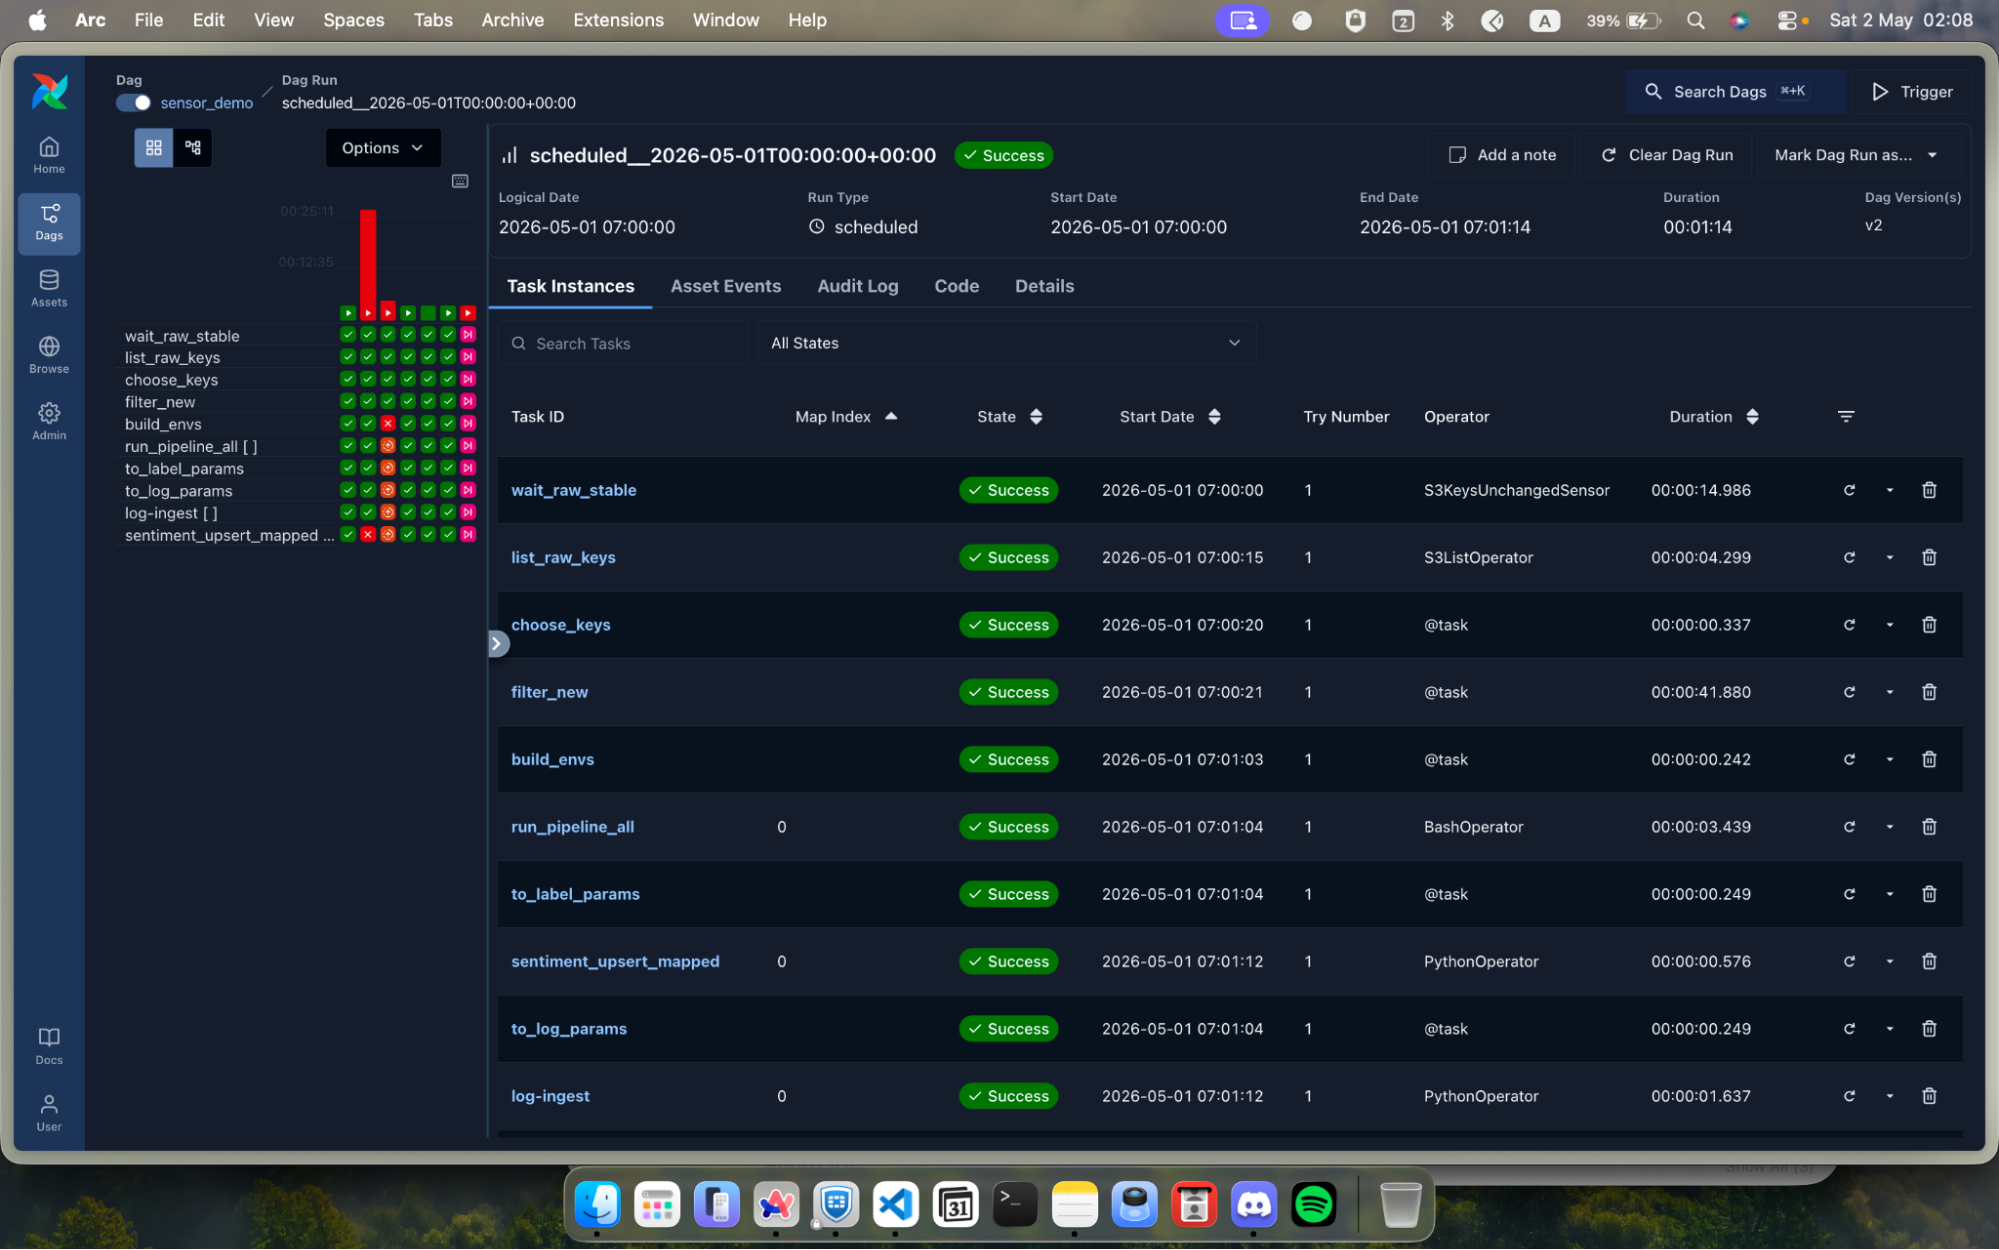
\includegraphics[width=0.95\textwidth]{figures/image19.png}
\caption{Main pipeline DAG}\label{fig:main-pipeline-dag}
\end{figure}

\clearpage
\subsection{Sentiment Processing Pipeline}

The second pipeline focuses on sentiment analysis and labeling of processed text data. The task \texttt{run\_sentiment\_from\_db} executes successfully using a \texttt{PythonOperator}. This demonstrates that the pipeline supports incremental processing and can continuously enrich datasets with labels, which is essential for supervised learning and model fine-tuning.

\begin{figure}[H]\centering
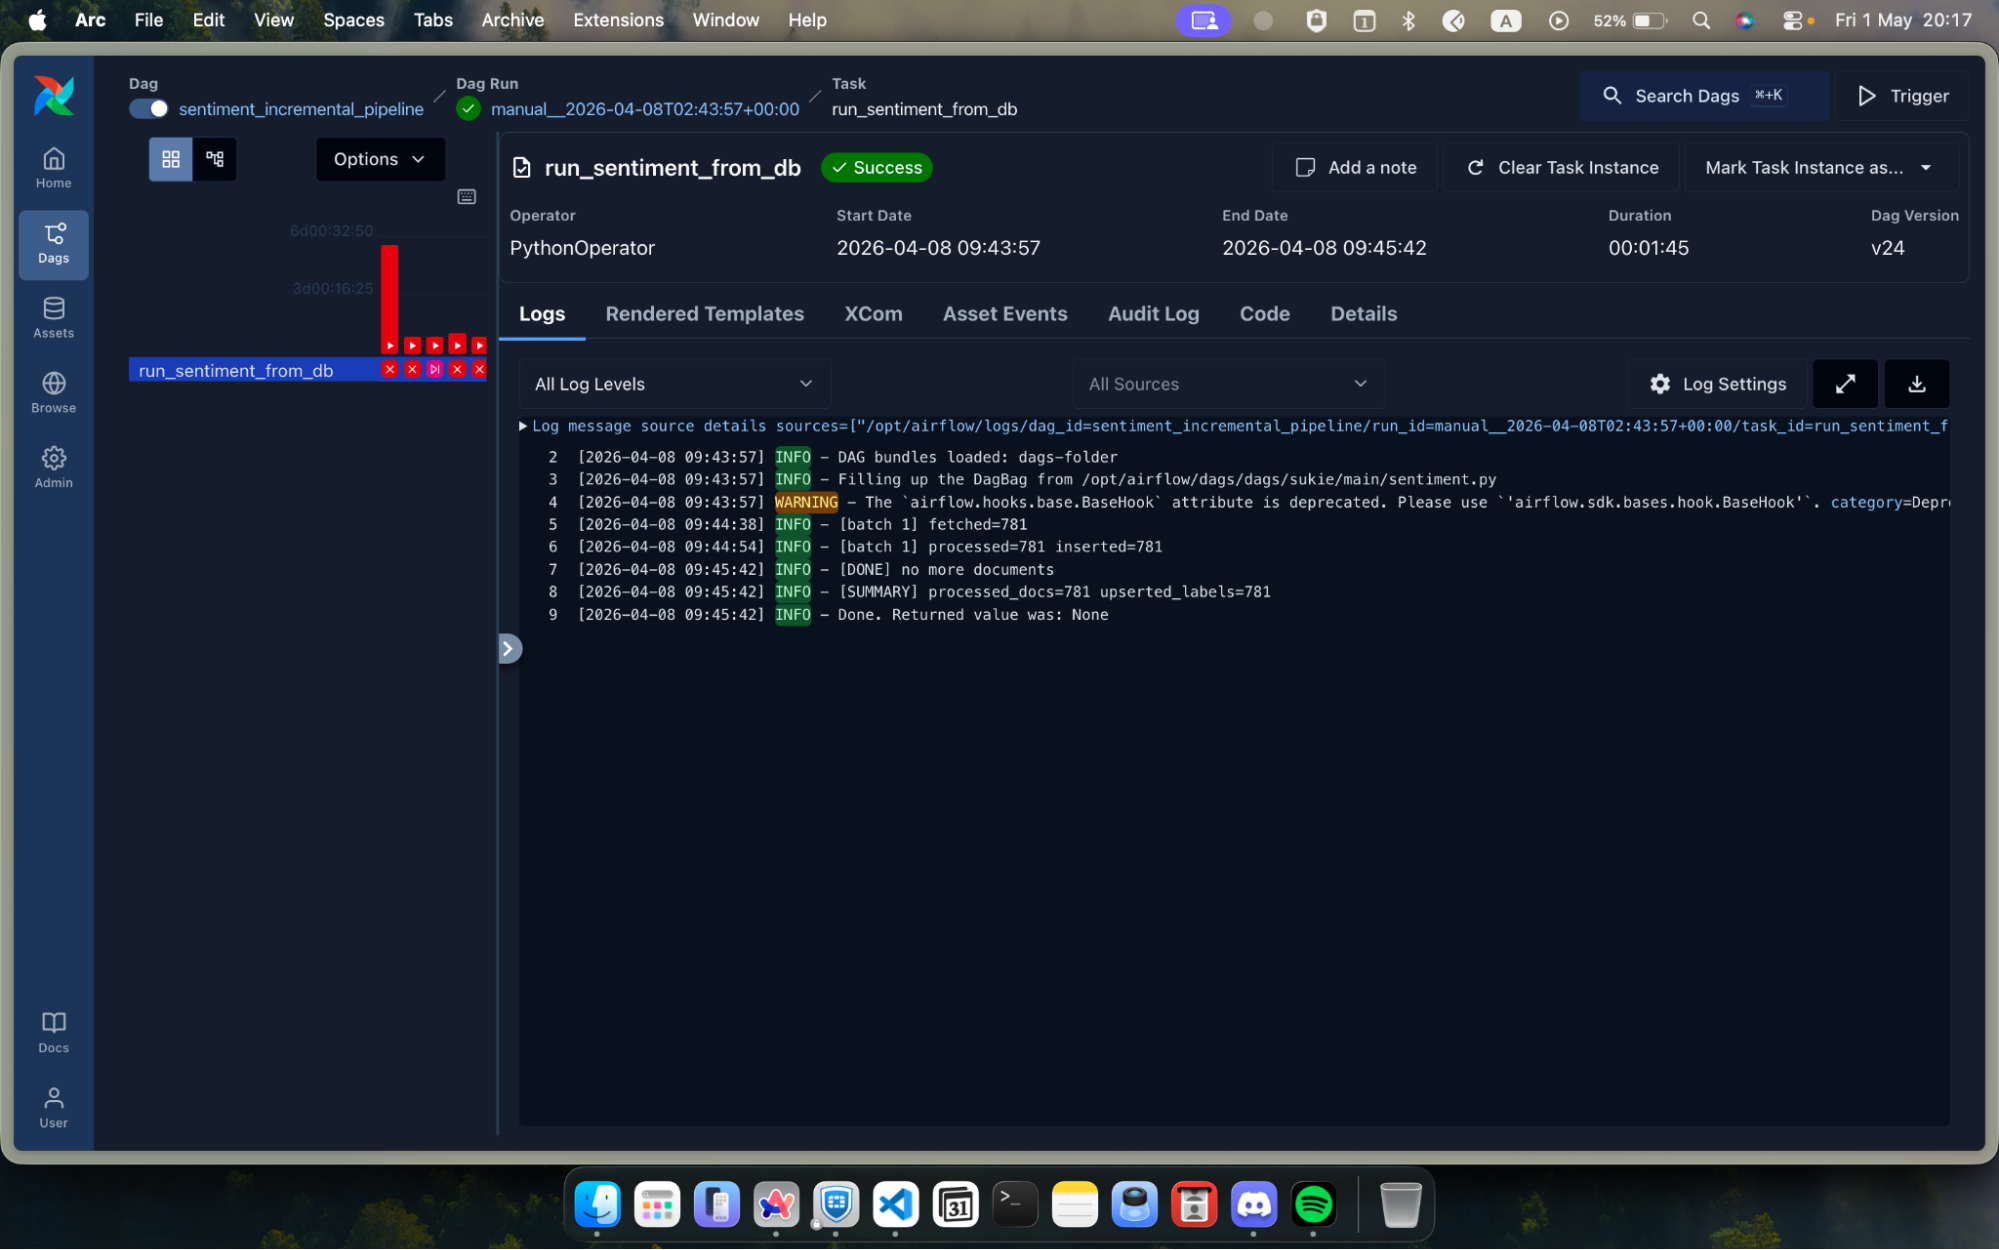
\includegraphics[width=0.95\textwidth]{figures/image4.png}
\caption{Sentiment Processing Pipeline}\label{fig:sentiment-pipeline}
\end{figure}

\clearpage
\section{Database}

This section presents the implementation and results of the PostgreSQL database used in the data ingestion and preparation pipeline. The database is designed to support structured storage of datasets, documents, labels and preprocessing logs, enabling efficient querying and monitoring of data processing workflows. The schema is designed with a relational structure consisting of multiple interconnected tables including \texttt{datasets}, \texttt{documents}, \texttt{labels} and \texttt{preprocessing\_logs}, which together support the full lifecycle of data ingestion, transformation and validation.

\begin{figure}[H]\centering
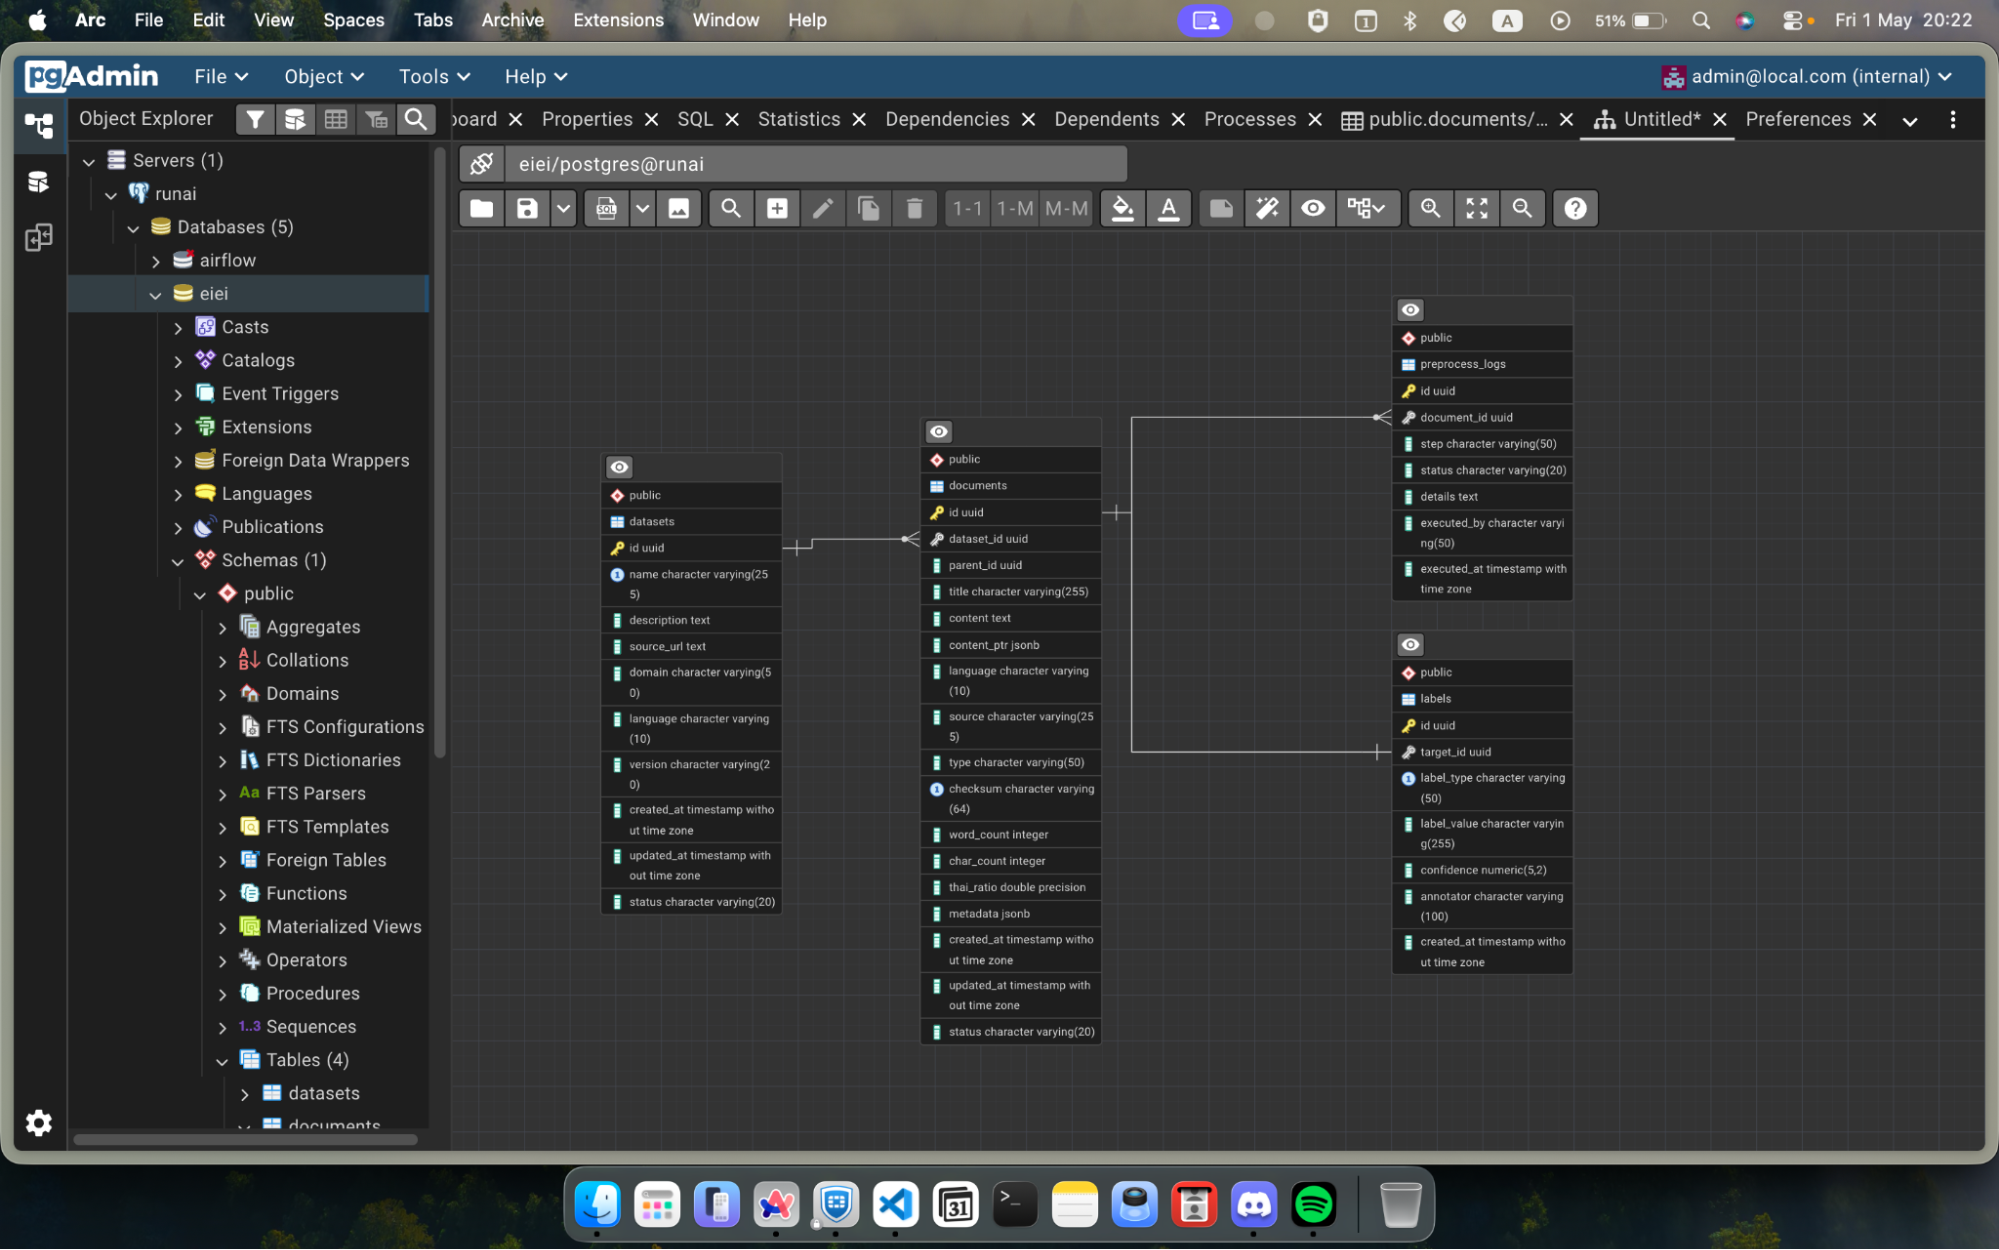
\includegraphics[width=0.95\textwidth]{figures/image5.png}
\caption{Database schema in PostgreSQL}\label{fig:db-schema-result}
\end{figure}

\subsection{Datasets}
The \texttt{datasets} table contains metadata describing each dataset ingested into the system. This includes dataset name, domain, language and version. This demonstrates that the pipeline is capable of handling diverse data sources and domains, which is essential for building generalized AI models. The dataset categorization also enables filtering and selection of data for specific use cases.

\begin{figure}[H]\centering
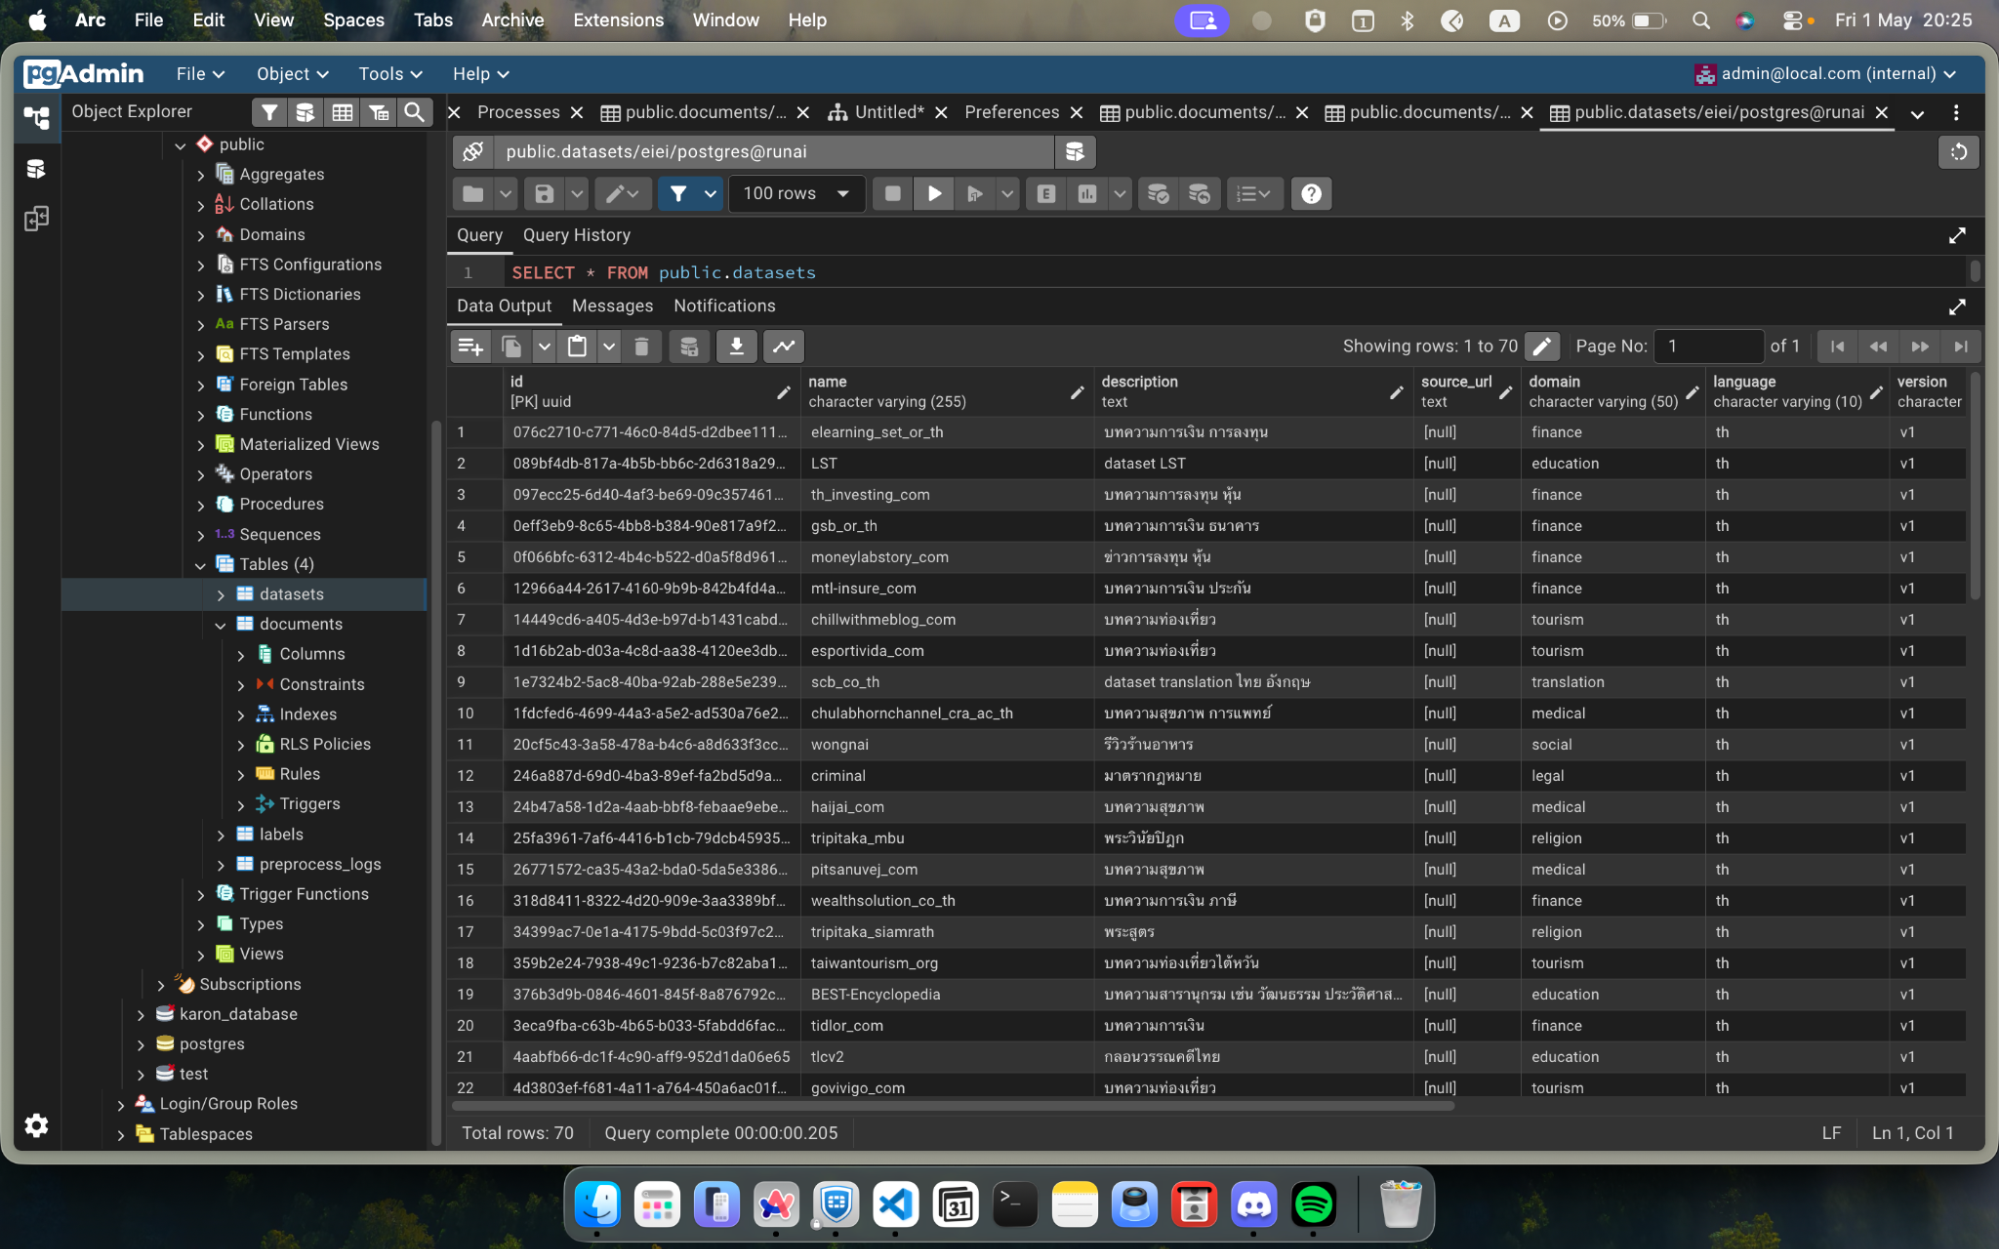
\includegraphics[width=0.95\textwidth]{figures/image32.png}
\caption{Dataset tables}\label{fig:datasets-table}
\end{figure}

\subsection{Documents}
The \texttt{documents} table stores the main textual data ingested from various sources. Each record represents a processed document with attributes such as dataset reference, content, language and metadata. The system successfully stores large volumes of text data extracted from multiple sources such as CC100, OSCAR and OpenSubtitles. The structured and cleaned text confirms that the ingestion and preprocessing pipeline successfully transforms raw data into AI-ready format.

\begin{figure}[H]\centering
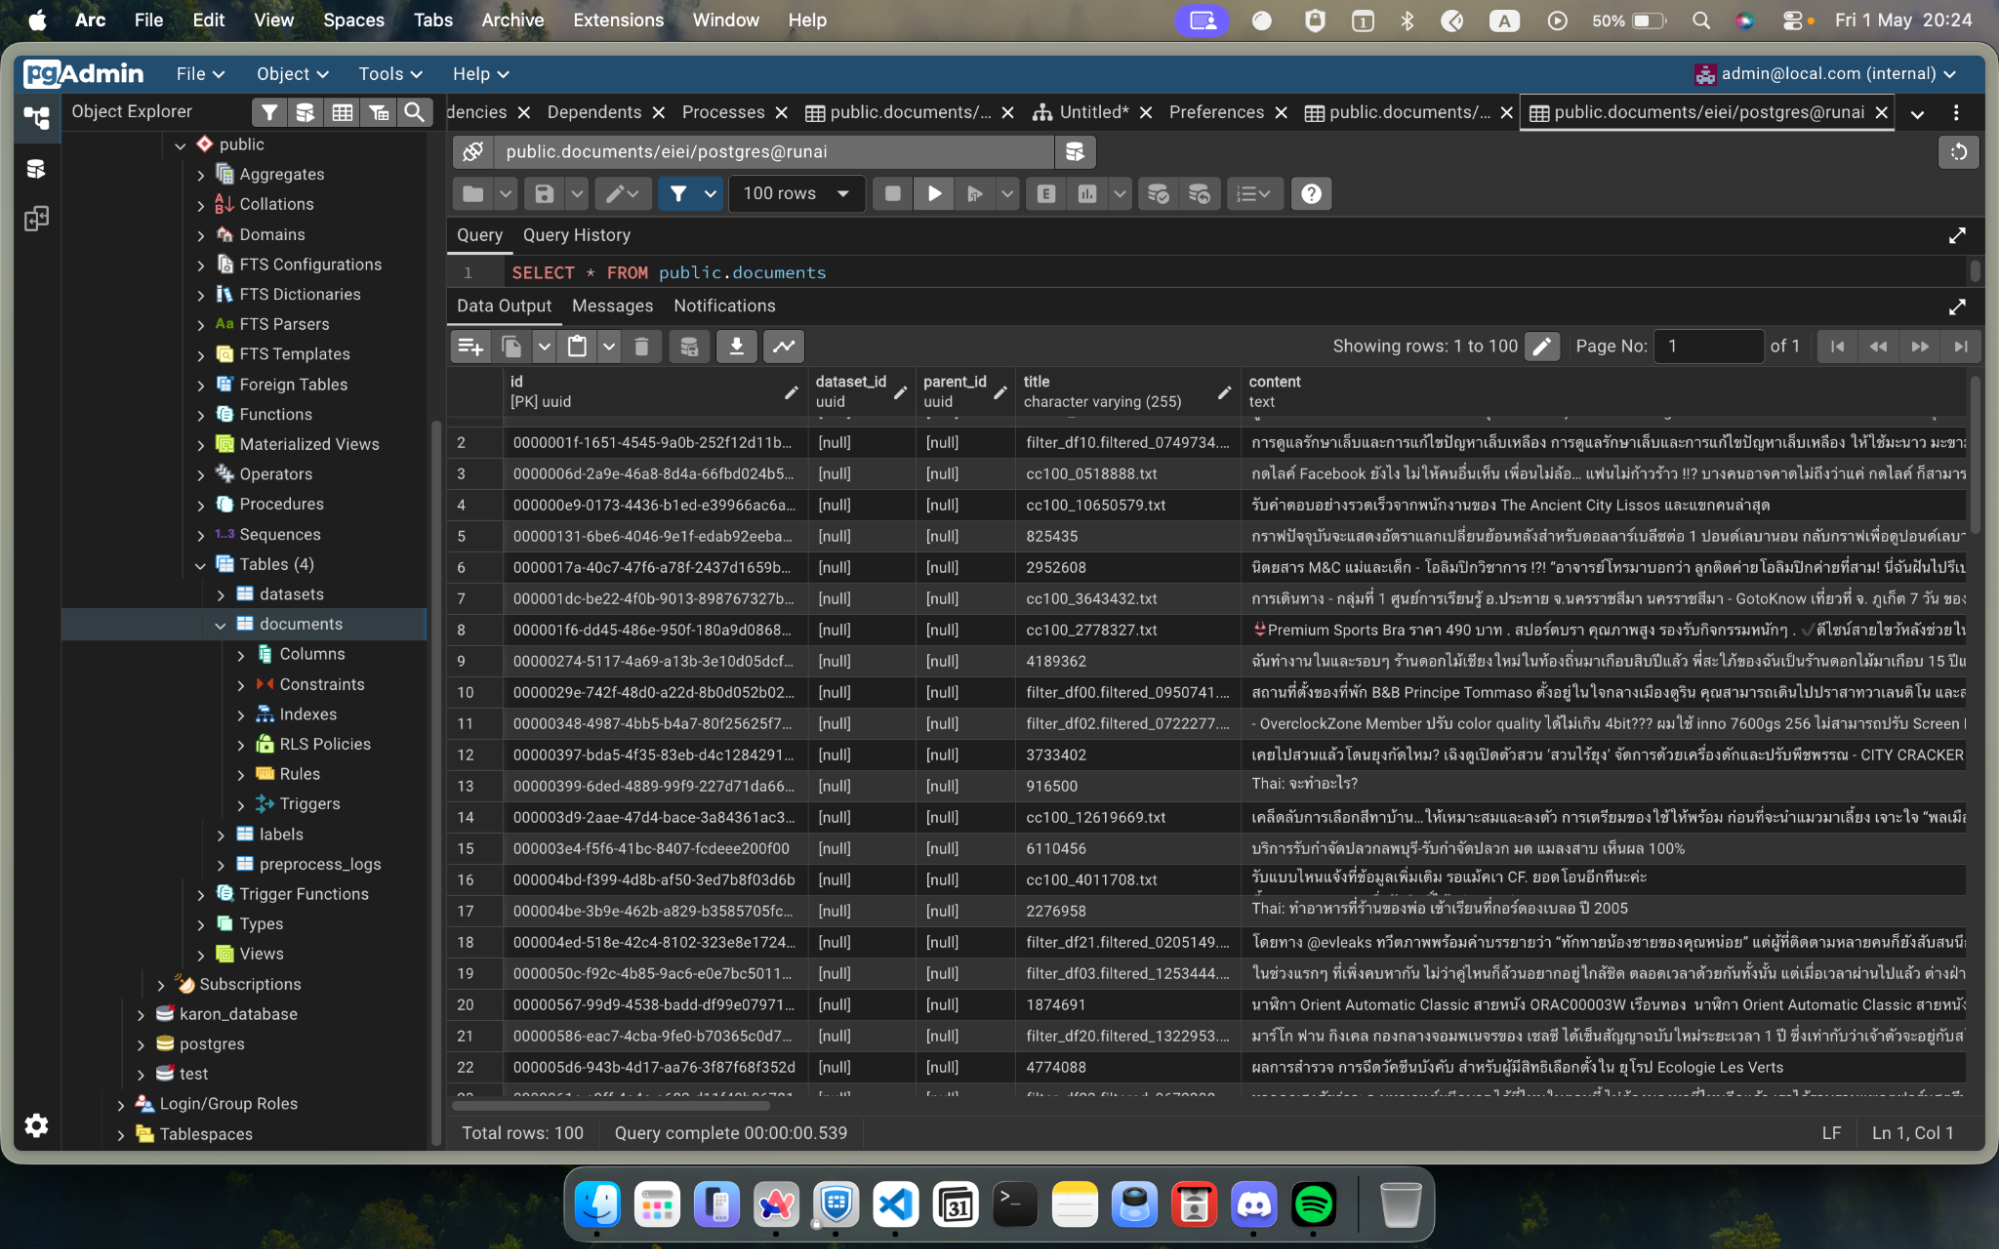
\includegraphics[width=0.95\textwidth]{figures/image10.png}
\caption{Document Table}\label{fig:documents-table}
\end{figure}

\begin{figure}[H]\centering
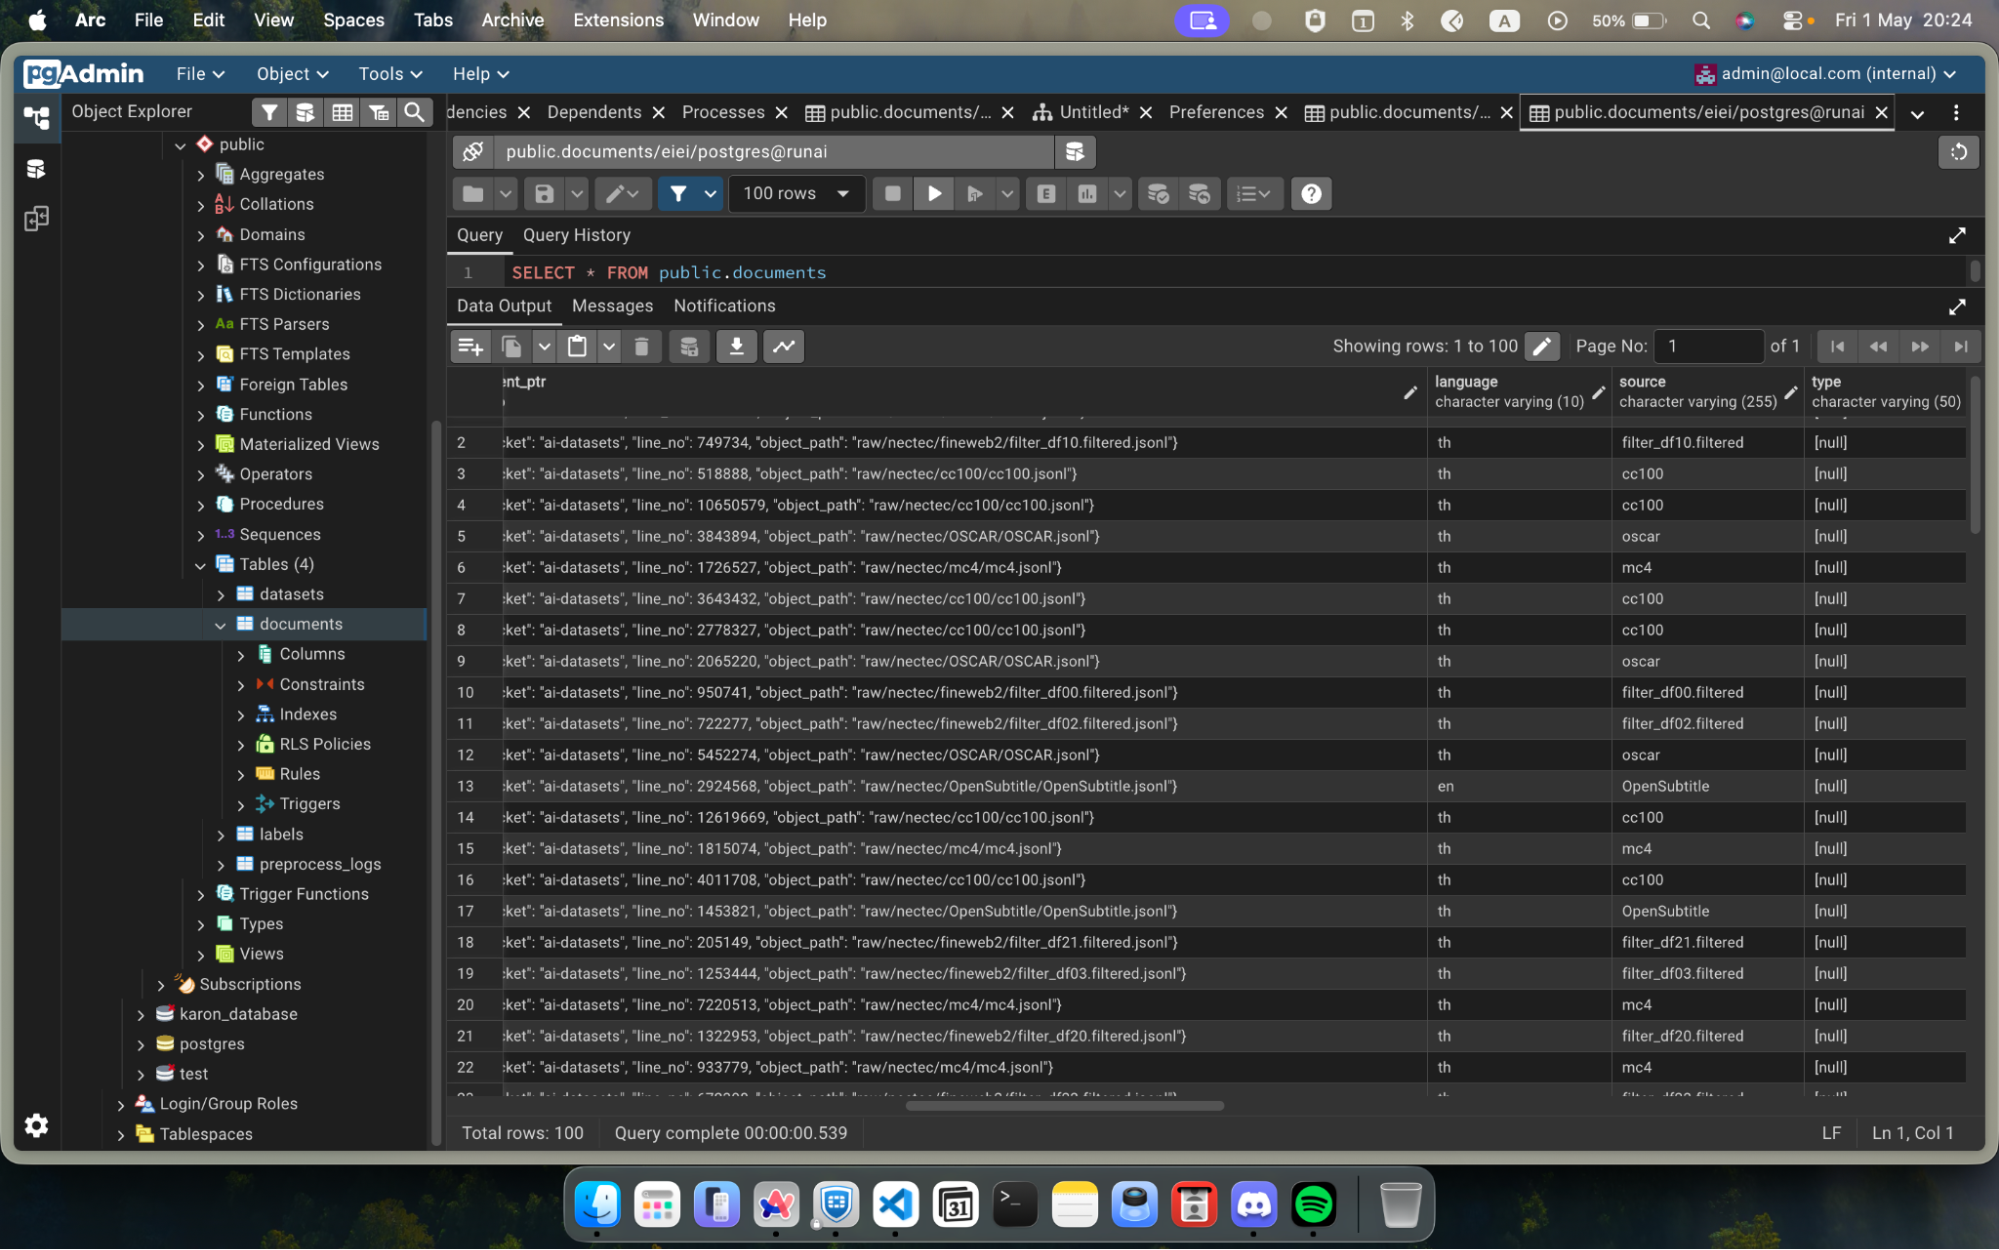
\includegraphics[width=0.95\textwidth]{figures/image20.png}
\caption{Document Table (detail view)}\label{fig:documents-table2}
\end{figure}

\subsection{Labels}
The \texttt{labels} table is used for storing annotation results such as sentiment classification. Each label is linked to a specific document or message via \texttt{target\_id}. This indicates that the system supports supervised learning workflows and can be used for fine-tuning AI models. The inclusion of confidence scores allows further filtering of high-quality labeled data.

\begin{figure}[H]\centering
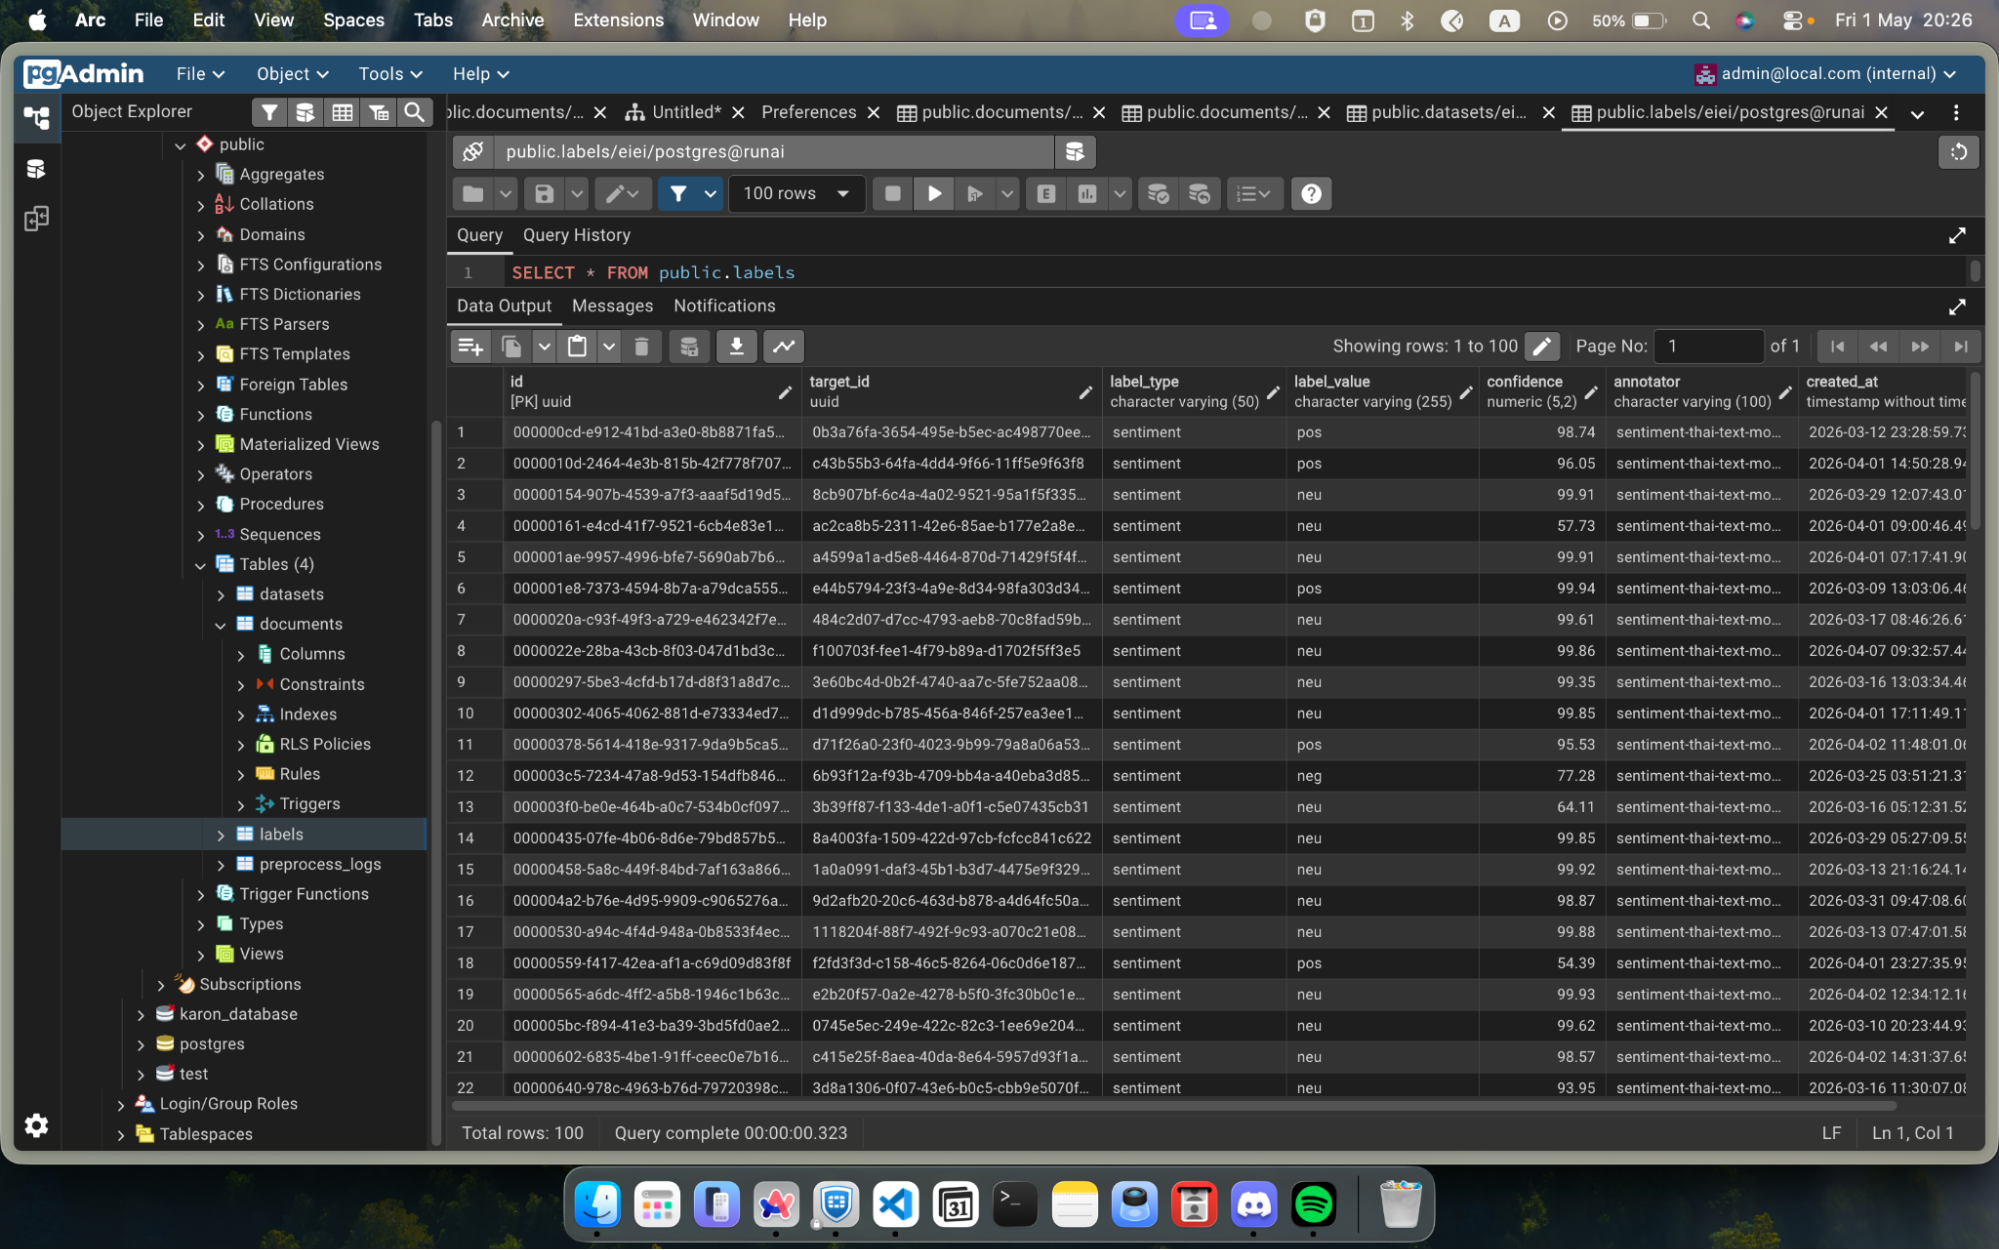
\includegraphics[width=0.95\textwidth]{figures/image12.png}
\caption{Labels Table}\label{fig:labels-table}
\end{figure}

\subsection{preprocessing\_logs}
The \texttt{preprocessing\_logs} table records all steps performed during the data cleaning pipeline. This includes operations such as input validation, HTML removal and text normalization. Each log entry contains a step describing the preprocessing stage and a status indicating success or failure. Most preprocessing steps were successfully executed, with detailed logs recorded for traceability. This provides transparency and makes it easier to debug errors or analyze pipeline performance.

\begin{figure}[H]\centering
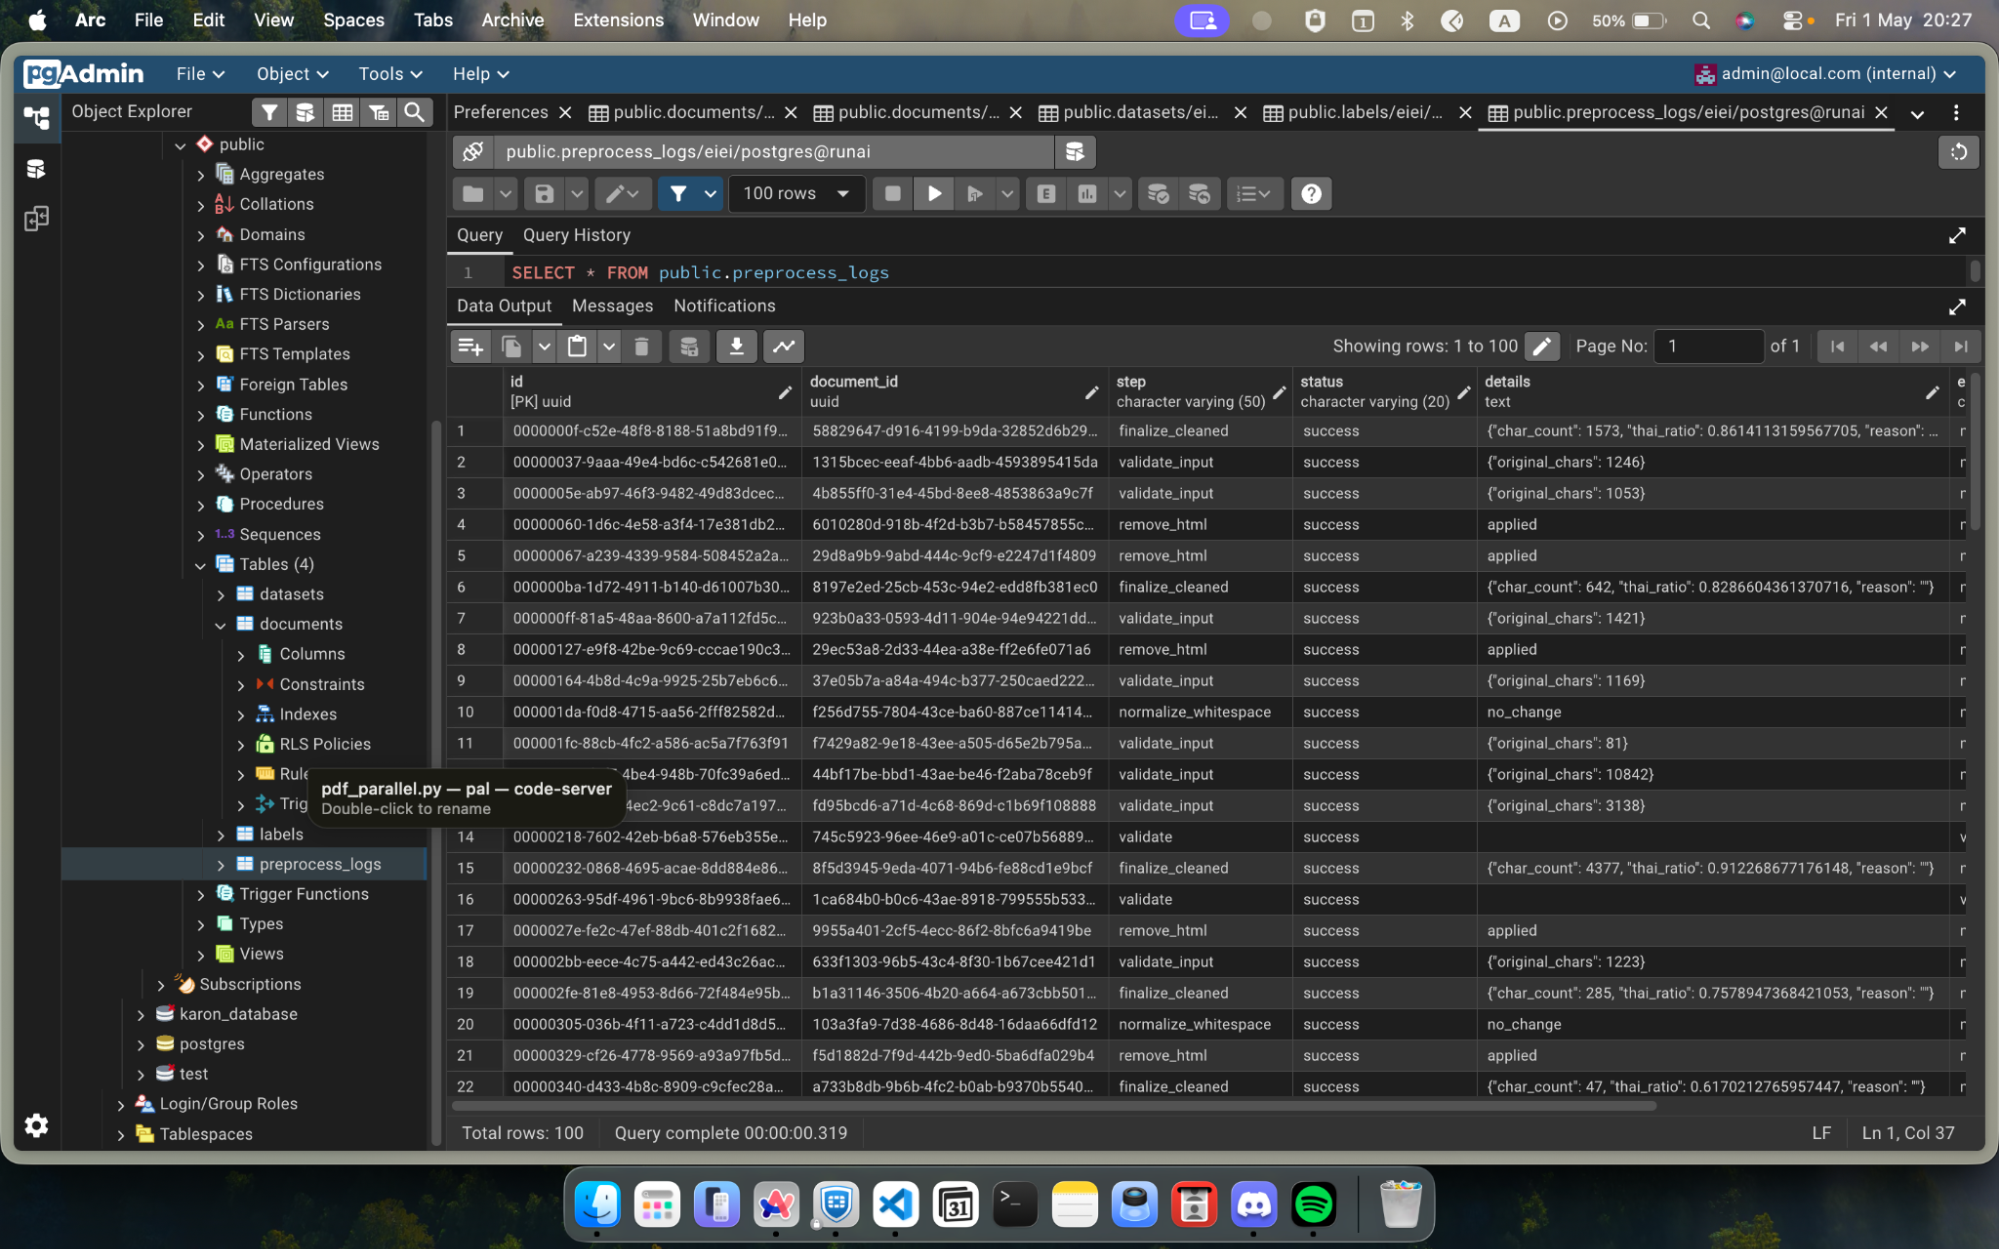
\includegraphics[width=0.95\textwidth]{figures/image8.png}
\caption{Preprocessing\_logs Table}\label{fig:preplogs-table}
\end{figure}

\section{Dashboard}

The monitoring dashboard developed in this project plays a critical role in ensuring the reliability, performance and data quality of the entire data pipeline. By integrating multiple components including Airflow, MinIO and PostgreSQL, the system provides a comprehensive view of pipeline execution, storage usage and database performance.
\newpage
\subsection{Airflow Dashboards}
For the Airflow cluster, the dashboard tracks DAG success/failure rate, task duration, number of running tasks and scheduler health. These panels help detect failed runs or unusually slow tasks.

\begin{figure}[H]\centering
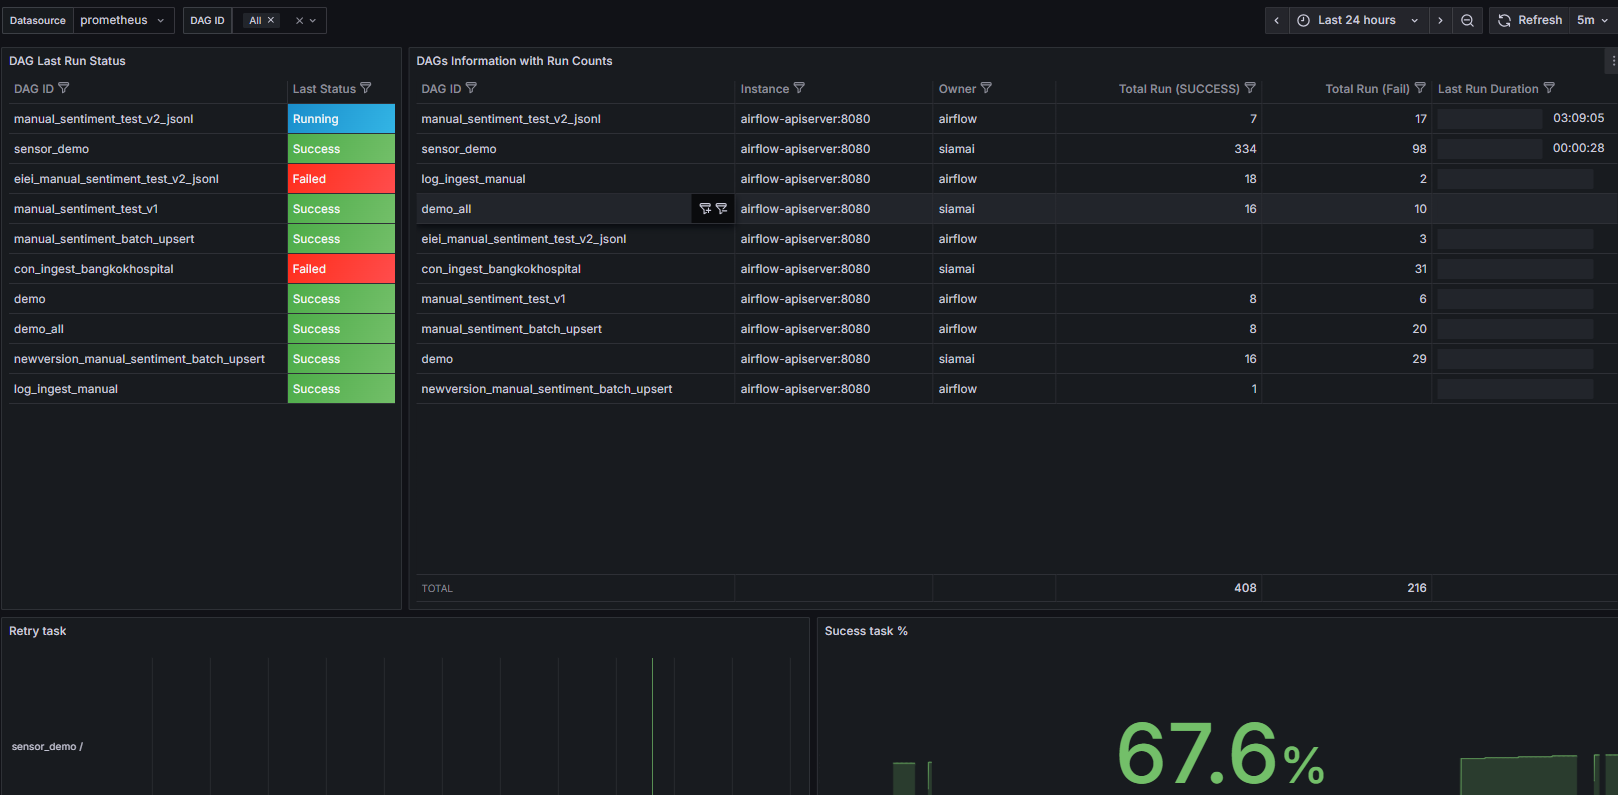
\includegraphics[width=0.95\textwidth]{figures/image24.png}
\caption{Airflow Dashboards}\label{fig:airflow-dash}
\end{figure}

\subsection{MinIO Dashboards}
The MinIO cluster and bucket dashboards show bucket size, number of objects, upload/download throughput and storage usage. This view is used to check whether data ingestion is growing as expected and whether there is enough storage left.

\begin{figure}[H]\centering
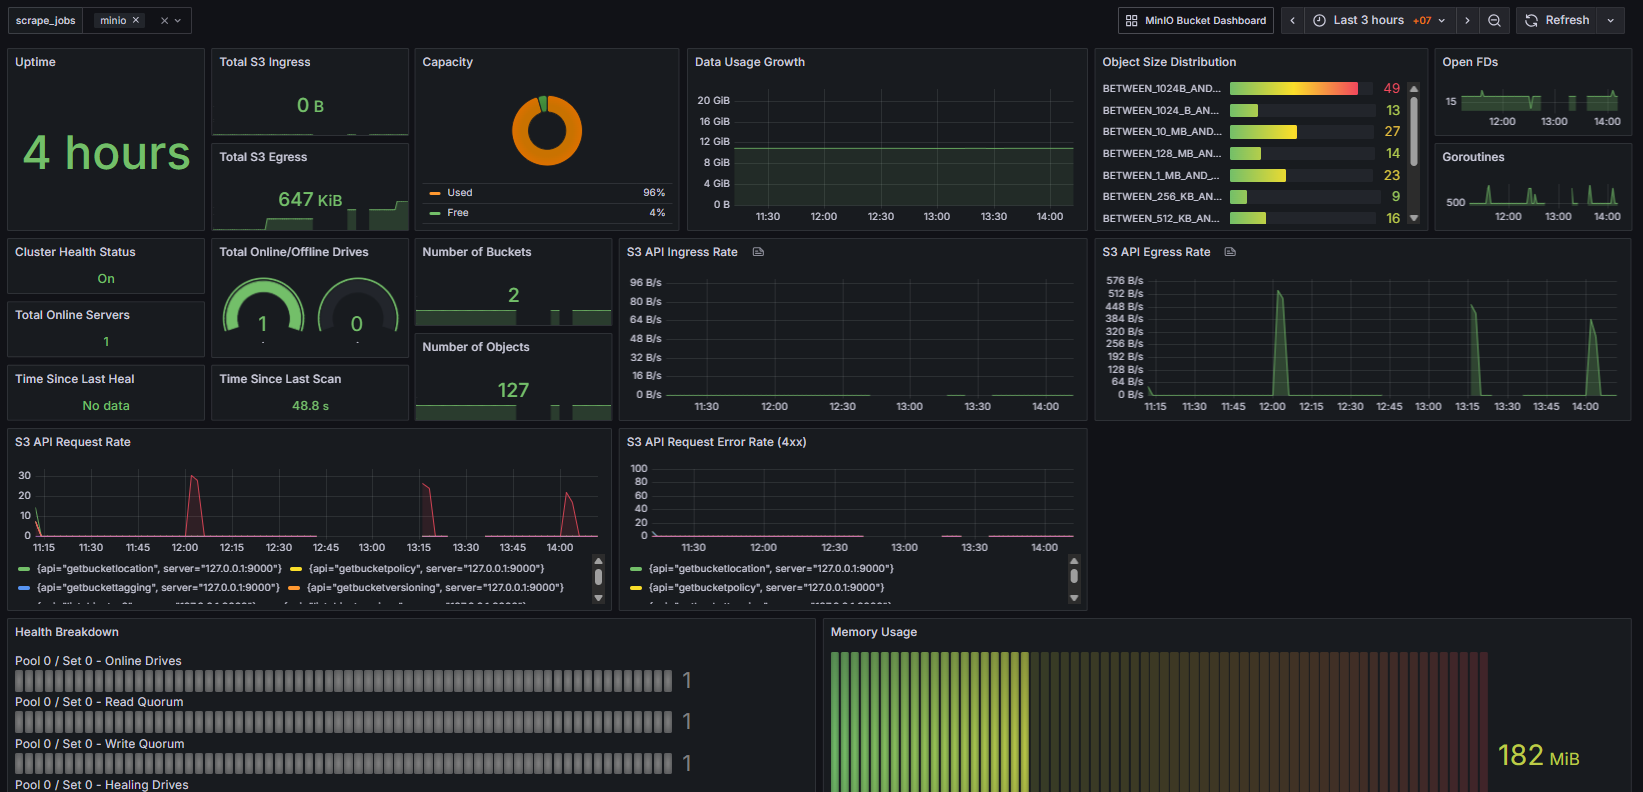
\includegraphics[width=0.95\textwidth]{figures/image11.png}
\caption{MinIO Dashboards}\label{fig:minio-dash}
\end{figure}
\newpage
\subsection{PostgreSQL}
The PostgreSQL database dashboard tracks query execution time, active connections, table size growth and other database metrics that may affect pipeline performance.

\begin{figure}[H]\centering
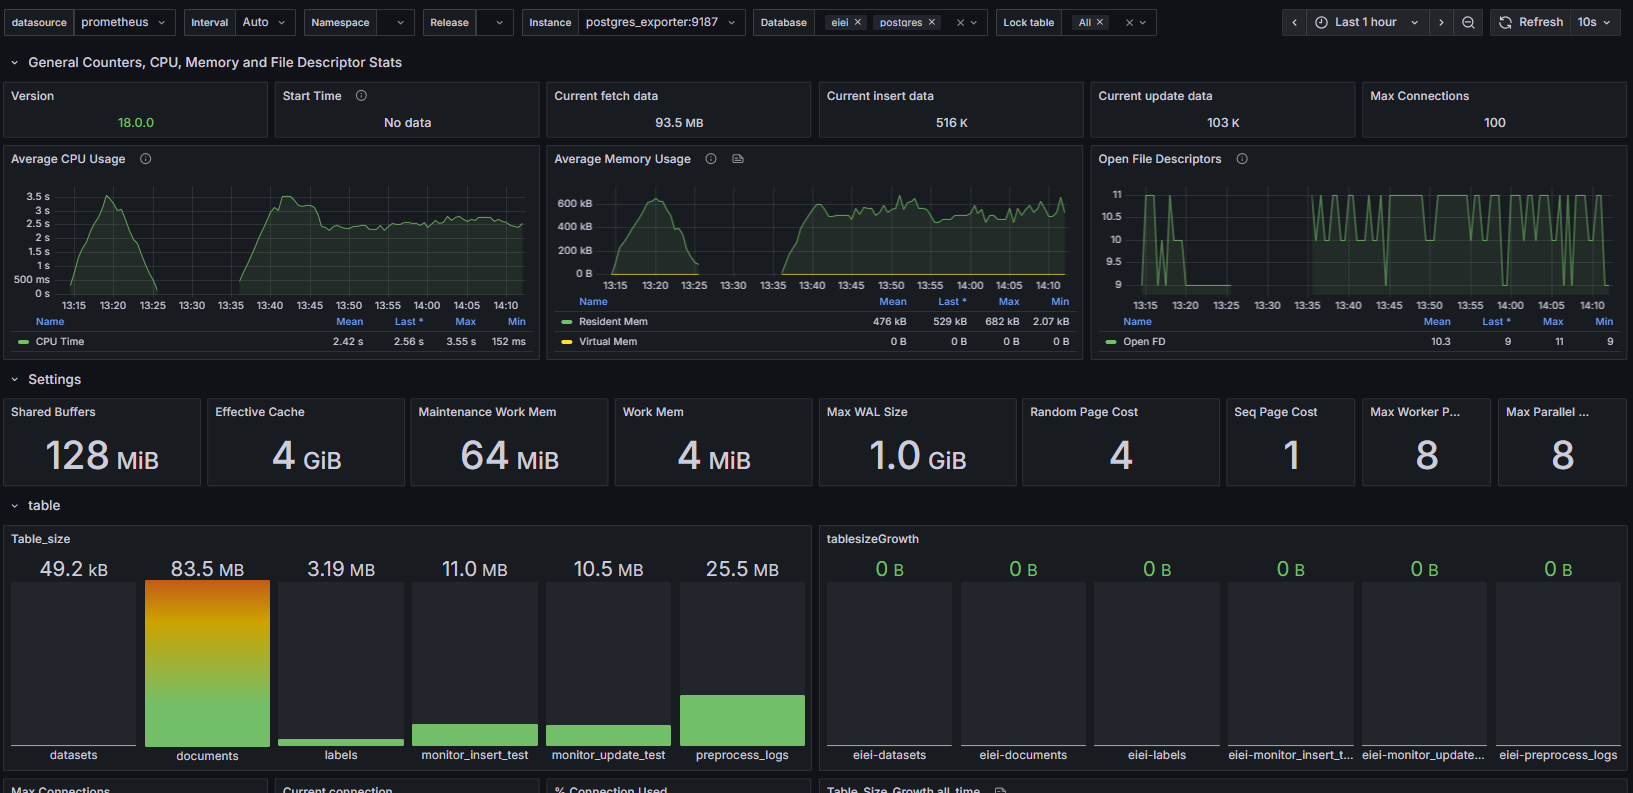
\includegraphics[width=0.95\textwidth]{figures/image7.png}
\caption{PostgreSQL Dashboards}\label{fig:postgres-dash}
\end{figure}

\subsection{Data Quality}
This is a custom dashboard that reads metrics generated from SQL queries through the Postgres exporter. It shows batch counts, number of cleaned records and other indicators derived from the \texttt{documents} and \texttt{preprocessing\_log} tables. These panels are used to check whether each batch was processed completely and to spot unusual drops or spikes in record counts.

\begin{figure}[H]\centering
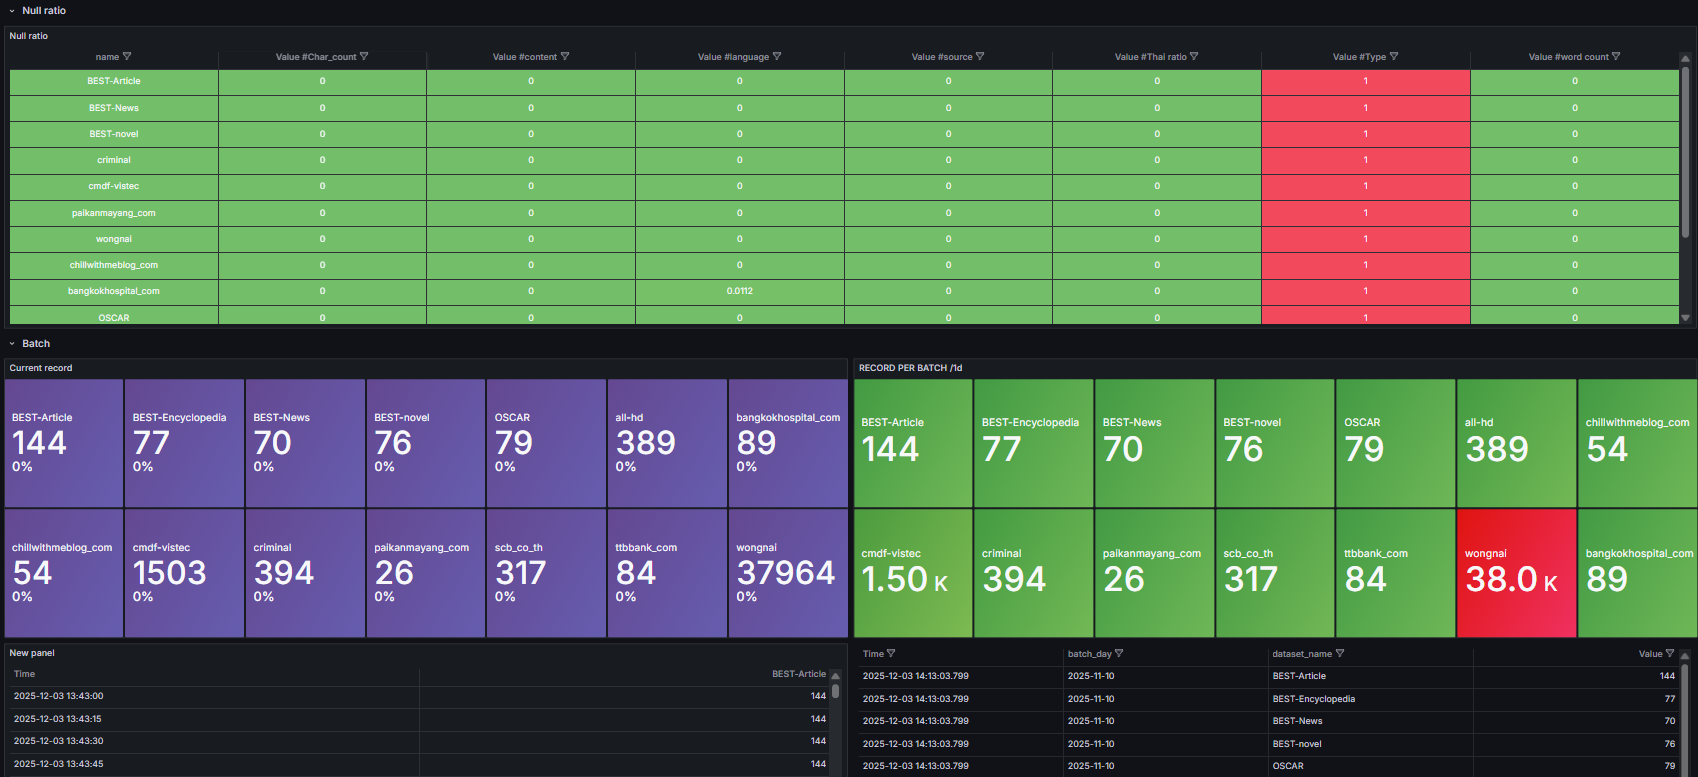
\includegraphics[width=0.95\textwidth]{figures/image28.png}
\caption{Data Quality Dashboards}\label{fig:dataquality-dash}
\end{figure}

%%%%%%%%%%%%%%%%%%%%%%%%%%%%%%%%%%%%%%%%%%%%%%%%%%%%%%%%%%%%%%
%%%%%%%%%%%%%%%  CHAPTER 5  %%%%%%%%%%%%%%%%%%%%%%%%%%%%%%%%%%
%%%%%%%%%%%%%%%%%%%%%%%%%%%%%%%%%%%%%%%%%%%%%%%%%%%%%%%%%%%%%%
\chapter{Conclusion}

\section{Conclusion}

This project developed an Automated Data Ingestion and Preparation Pipeline for AI Model Training. The main goal of the project was to design and implement a pipeline that can collect, process, clean, validate, store and monitor different types of data so that the final outputs are suitable for downstream AI model training.

The completed system consists of several main components: a Data Lake using MinIO, automated processing pipelines using Apache Airflow, a PostgreSQL database for metadata and processed data storage, an unstructured data pipeline for PDF and audio processing, and a monitoring dashboard for system and data quality tracking. The MinIO data lake was organized into multiple layers to support raw, cleaned, processed and validated data storage. This structure helps separate each stage of the pipeline and makes the system easier to extend when new datasets are added.

For the unstructured pipeline, the PDF pipeline successfully processed 133 PDF documents with 7{,}346 pages, producing approximately 8.42 million characters of extracted Thai text. The audio pipeline processed 335{,}674 audio records, kept 307{,}793 valid transcripts and generated approximately 19.42 million characters from 656.93 hours of audio. In total, the PDF and audio pipelines produced approximately 27.85 million characters of AI-ready text data.

The PDF pipeline achieved a 100\% document-level success rate and a 95.2\% page-level success rate. The hybrid extraction method, which combines PyMuPDF and OCR, was effective because it allowed the system to process text-native PDFs efficiently while still extracting text from image-heavy PDFs. The audio pipeline also achieved strong results, with a 91.69\% acceptance rate, a mean CER of 0.0447 and no failed or server-empty records in the final output. In addition, the audio format compatibility test confirmed that the pipeline could process 13 common audio formats, with 26 out of 26 format-clip trials successfully decoded and transcribed.

The system also includes a PostgreSQL database for storing datasets, documents, labels and preprocessing logs. This supports traceability, querying and future AI model training workflows. The dashboard provides visibility into Airflow, MinIO, PostgreSQL and data quality metrics. Overall, the project successfully achieved its main objective of building an automated pipeline that can transform raw data into clean, validated and AI-ready formats.

\begin{table}[H]
\centering
\caption{Project completion status}\label{tbl:completion}
\begin{tabular}{|p{0.28\textwidth}|p{0.45\textwidth}|p{0.18\textwidth}|}
\hline
\textbf{Component} & \textbf{Description} & \textbf{Status} \\ \hline
Data Lake & MinIO bucket structure for raw, cleaned, processed and validated data & Complete \\ \hline
PDF Pipeline & Extracts Thai text using PyMuPDF and OCR & Complete \\ \hline
Audio Pipeline & Converts Thai speech into text using ASR and filters by CER & Complete \\ \hline
Audio Format Compatibility & Supports WAV, MP3, M4A, OGG, WebM, WMA, 3GP, etc. & Complete \\ \hline
JSONL Pipeline & Processes JSONL/text datasets and stores cleaned outputs & Complete \\ \hline
Sentiment Processing & Adds sentiment labels to processed text data & Partially Complete \\ \hline
PostgreSQL Database & Stores datasets, documents, labels and preprocessing logs & Complete \\ \hline
Monitoring Dashboard & Tracks Airflow, MinIO, PostgreSQL and data quality metrics & Complete \\ \hline
Real-time Streaming Pipeline & Kafka-based real-time ingestion & Out of Scope \\ \hline
Model Training & Direct AI/LLM training and fine-tuning & Out of Scope \\ \hline
\end{tabular}
\end{table}

\section{Problems, Obstacles and Solutions}

During the project development, several problems and obstacles were encountered. These problems were mainly related to inconsistent data formats, Thai-language data quality and system performance when processing large-scale datasets. This section explains the main issues and how they were solved.

\subsection{Inconsistent Data Format Across Sources}

One major problem was that the input data came from many different formats and sources. The NECTEC text datasets included JSONL, TXT, CSV and PDF files. Some PDF documents were text-native, while others were scanned or image-heavy. The audio data also appeared in different container and codec formats such as WAV, MP3, M4A, OGG, WebM, WMA and 3GP. This inconsistency made it difficult to use one single processing method for all data.

To solve this problem, the system used a format-aware ingestion strategy. For PDFs, the pipeline first attempted direct text extraction using PyMuPDF. If the page did not contain usable embedded text, the pipeline used OCR as a fallback method. For audio data, the pipeline decoded different file formats using FFmpeg-backed tools and converted them into a common 16~kHz mono PCM WAV format before ASR processing. As a result, the ASR server only needed to process one standardized audio format.

The format compatibility test confirmed that this solution worked successfully. The pipeline processed 13 different audio formats across two test clips, and all 26 trials were successfully decoded and transcribed.

\subsection{Data Quality Issues in Thai Language Processing}

Another major challenge was data quality, especially for Thai-language processing. Thai text can be difficult to process because words are not always separated by spaces. In addition, OCR and ASR outputs may contain incorrect characters, repeated characters, missing tone marks, wrong transcriptions or hallucinated text.

For the PDF pipeline, some pages produced low-quality OCR outputs or no usable text at all. To prevent this, the system applied quality checks such as Thai-character ratio filtering, detection of abnormal repeated characters and filtering of corrupted or invalid characters. Empty pages and low-quality pages were excluded from the final output.

For the audio pipeline, transcription quality was evaluated using Character Error Rate (CER) instead of Word Error Rate (WER). CER was selected because it is more suitable for Thai text, where word boundaries are not always clear. Records with CER less than or equal to 0.20 were accepted. Silent audio detection was also added to remove clips that did not contain meaningful speech. These quality control methods helped improve the reliability of the final dataset.

\subsection{System Performance and Scalability Issues}

Processing large datasets created performance and scalability challenges. The PDF pipeline processed thousands of pages and OCR was computationally expensive. The audio pipeline processed more than 335{,}000 audio records, which required ASR inference and quality validation.

To reduce unnecessary computation, the PDF pipeline used PyMuPDF as the first extraction method and only used OCR when needed. For the audio pipeline, the system processed the dataset in Parquet shards and applied batch processing through the ASR workflow. The results across all 16 shards were consistent, with less than 1\% variation in major metrics.

Monitoring was also added to help manage performance issues. The dashboard provides visibility into Airflow task status, MinIO storage usage, PostgreSQL performance and data quality metrics. This makes it easier to identify failed tasks, slow processing steps, storage growth and unusual changes in processed record counts.

\section{Future Work and Suggestions}

Although the project achieved its main objectives, there are several ways the system could be improved and extended in the future.

\begin{itemize}
\item \textbf{Vision-based PDF fallback}: The PDF pipeline could be improved by adding a stronger vision-based fallback method for pages that are currently classified as empty. A more advanced layout-aware OCR or document understanding model could help recover more content.
\item \textbf{Audio quality tiers}: The audio pipeline could be extended by adding multiple quality tiers. Currently, the system uses a strict CER threshold of 0.20. Records with CER between 0.20 and 0.30 may still be usable for certain AI tasks, but they are excluded to keep the dataset precise.
\item \textbf{CER and WER reporting}: The system could include both CER and WER reporting after integrating a reliable Thai word segmentation tool, especially for ASR benchmarking.
\item \textbf{Unified database schema}: The schema could be further unified so that outputs from different modalities, such as PDF documents, JSONL records and audio transcripts, share a common structure with fields such as filename, source, content, quality score, processing method and validation status.
\item \textbf{Detailed alerts and notifications}: The monitoring dashboard could be extended with more detailed alerts and automated notifications. The system could send alerts when a pipeline fails, when storage usage becomes too high, when the number of low-quality records increases suddenly or when processing time becomes abnormal.
\item \textbf{Direct model training integration}: Future work could include direct integration with AI model training or fine-tuning workflows. The cleaned datasets could be connected to training frameworks such as Hugging Face Datasets, PyTorch or TensorFlow to support end-to-end AI development.
\end{itemize}

%%%%%%%%%%%%%%%%%%%%%%%%%%%%%%%%%%%%%%%%%%%%%%%%%%%%%%%%%%%%%%%
%%%%%%%%%%%%%%%%%%%% Bibliography %%%%%%%%%%%%%%%%%%%%%%%%%%%%%
%%%%%%%%%%%%%%%%%%%%%%%%%%%%%%%%%%%%%%%%%%%%%%%%%%%%%%%%%%%%%%%
\makeatletter
\g@addto@macro{\UrlBreaks}{\UrlOrds}
\makeatother

\begin{thebibliography}{99}

\bibitem{huyen2024} Huyen, C. (2024). \textit{AI engineering: Building applications with foundation models}. O'Reilly Media.

\bibitem{airbyte} Airbyte. (n.d.). \textit{Open-source data integration}. Retrieved August 20, 2025, from \url{https://airbyte.com/}

\bibitem{aws-s3} Amazon Web Services. (n.d.). \textit{Amazon S3}. Retrieved August 22, 2025, from \url{https://aws.amazon.com/s3/}

\bibitem{airflow} Apache Airflow. (n.d.). \textit{Apache Airflow documentation}. Retrieved August 22, 2025, from \url{https://airflow.apache.org/docs/apache-airflow/stable/}

\bibitem{arrow} Apache Arrow. (n.d.). \textit{Apache Arrow documentation}. Retrieved August 18, 2025, from \url{https://arrow.apache.org/}

\bibitem{kafka} Apache Kafka. (n.d.). \textit{Apache Kafka documentation}. Retrieved August 18, 2025, from \url{https://kafka.apache.org/}

\bibitem{nifi} Apache NiFi. (n.d.). \textit{Apache NiFi project}. Retrieved August 18, 2025, from \url{https://nifi.apache.org/}

\bibitem{git} Chacon, S., \& Straub, B. (2014). \textit{Pro Git} (2nd ed.). Apress. \url{https://git-scm.com/book/en/v2}

\bibitem{docker} Docker. (n.d.). \textit{What is Docker?} Retrieved August 13, 2025, from \url{https://www.docker.com/resources/what-container}

\bibitem{forticlient} Fortinet. (n.d.). \textit{FortiClient VPN}. Retrieved August 14, 2025, from \url{https://www.fortinet.com/products/endpoint-security/forticlient}

\bibitem{grafana} Grafana Labs. (n.d.). \textit{What is Grafana?} Retrieved August 19, 2025, from \url{https://grafana.com/}

\bibitem{bigquery} Google Cloud. (n.d.). \textit{BigQuery}. Retrieved August 15, 2025, from \url{https://cloud.google.com/bigquery}

\bibitem{easyocr} JaidedAI. (n.d.). \textit{EasyOCR}. Retrieved September 17, 2025, from \url{https://github.com/JaidedAI/EasyOCR}

\bibitem{pandas} McKinney, W. (2010). Data structures for statistical computing in Python. \textit{Proceedings of the 9th Python in Science Conference}, 56--61. \url{https://pandas.pydata.org/}

\bibitem{vscode} Microsoft. (n.d.). \textit{Visual Studio Code}. Retrieved August 13, 2025, from \url{https://code.visualstudio.com/}

\bibitem{minio} MinIO. (n.d.). \textit{High performance object storage}. Retrieved August 14, 2025, from \url{https://min.io/}

\bibitem{paddleocr} PaddleOCR Contributors. (n.d.). \textit{PaddleOCR}. Retrieved September 12, 2025, from \url{https://github.com/PaddlePaddle/PaddleOCR}

\bibitem{postgres} PostgreSQL Global Development Group. (n.d.). \textit{PostgreSQL: The world's most advanced open source database}. Retrieved August 18, 2025, from \url{https://www.postgresql.org/}

\bibitem{prometheus} Prometheus Authors. (n.d.). \textit{Prometheus monitoring system}. Retrieved August 18, 2025, from \url{https://prometheus.io/}

\bibitem{pythainlp} Phatthiyaphaibun, W., et al. (2023). PyThaiNLP: Thai natural language processing in Python. \textit{Proceedings of the 3rd Workshop for NLP-OSS}, 25--36. \url{https://aclanthology.org/2023.nlposs-1.4/}

\bibitem{tesseract} Smith, R. (2007). An overview of the Tesseract OCR engine. \textit{Proceedings of the International Conference on Document Analysis and Recognition (ICDAR)}, 629--633. \url{https://doi.org/10.1109/ICDAR.2007.4376991}

\bibitem{typhoonocr} Typhoon OCR. (n.d.). \textit{Typhoon OCR project}. Retrieved September 15, 2025, from \url{https://github.com/scb-10x/typhoon-ocr}

\bibitem{typhoonisan} Typhoon AI. (n.d.). \textit{Typhoon Isan ASR Whisper}. Hugging Face. Retrieved October 10, 2025, from \url{https://huggingface.co/typhoon-ai/typhoon-isan-asr-whisper}

\bibitem{typhoonocr7b} Typhoon AI. (n.d.). \textit{Typhoon OCR 7B}. Hugging Face. Retrieved September 15, 2025, from \url{https://huggingface.co/typhoon-ai/typhoon-ocr-7b}

\bibitem{nvidia-b200} NVIDIA Corporation. (n.d.). \textit{NVIDIA DGX B200}. Retrieved September 15, 2025, from \url{https://www.nvidia.com/en-us/data-center/dgx-b200/}

\bibitem{wangchanberta} AIResearch. (2021, March 3). \textit{WangchanBERTa: Pre-trained Thai language model}. Retrieved October 4, 2025, from \url{https://airesearch.in.th/releases/wangchanberta-pre-trained-thai-language-model/}

\end{thebibliography}

\end{document}
